
\documentclass[12pt,a4paper]{article}
\usepackage[margin=1in]{geometry} 
\usepackage{amsmath,hyperref,listings,blindtext,csquotes,titlesec,amsthm,amssymb,graphicx,mathtools,scrextend,tikz,hyperref,algorithm2e, enumitem}


\usepackage{float}
\usepackage{booktabs,dcolumn} % ,caption}
\usepackage{varwidth ,wrapfig,lipsum}
\usepackage{vhistory}


% %
% \captionsetup{%labelsep=newline,
%               singlelinecheck=false,
%               skip=0.333\baselineskip}
              
% \DeclareCaptionFormat{myformat}{\fontsize{8}{8}\selectfont#1#2#3}
% \captionsetup[figure]{format=myformat}
% \captionsetup[table]{format=myformat}


\usepackage{multicol}

\usetikzlibrary{positioning}

\usepackage[nottoc]{tocbibind}

\graphicspath{{images/}}

\newcommand\teo[1]{\textcolor{blue}{#1}}

\lstset{ 
  backgroundcolor=\color{white},  
  basicstyle=\scriptsize,
  mathescape=true, frame=single,
   numbers=left,
  numbersep=5pt,
  }

\setcounter{secnumdepth}{4}
\hypersetup{
	colorlinks=true,
	linkcolor=black,
	filecolor=magenta,      
	urlcolor=cyan,
}




\begin{document}

\begin{titlepage}
	\centering
	
\includegraphics[width=0.45\textwidth]{images/polimi.png}\par\vspace{1cm}
	{\scshape\LARGE Politecnico di Milano \par}
	\vspace{1cm}
	{\scshape\Large Artificial Neural Networks And Deep Learning \par}
	\vspace{1.5cm}
	{\LARGE\bfseries Notes\par}
	{\LARGE\bfseries a.a. 2019-2020\par}
	\vspace{0.7cm}
	{\textbf{Authors}\\
	\textbf{Alessio Russo Introito}: russointroitoa@gmail.com \\
	\textbf{Matteo Moreschini}: matmoresc@gmail.com \\
    }
	\vfill
	{\large \today\par}
\end{titlepage}

\section*{Contribution}

\subsection*{How to contribute}
Please follow these steps to keep track of changes and contributions:
\begin{enumerate}
    \item Add or modify the document where you need
    \item Add a small summary of your work into \textit{CHANGELOG.tex} (a hidden file to log contributions)
    \item Add your name in the following \textit{Contributors} section
\end{enumerate}

Contributions and reviews are welcome! Please, make sure your claims and changes are correct and well-described

\subsection*{Contributors}


\tableofcontents

\newpage

%\section{Machine Learning Basics}
What's a \textbf{machine learning algorithm}? Mitchell (1997) provides the following definition: 

\begin{displayquote}
    "\textit{A computer program is said to learn from experience E with respect to some class of tasks T and performance measure P, if its performance at tasks T, as measured by P, improves with experience E."}
\end{displayquote}

A machine learning \textbf{task} is usually described in terms of how the machine should process an example, which is a collection of features that have been quantitatively measured from some object or event that we want the machine learning system to process. There are several different tasks that can be involved in machine learning, the following two are the most important:
\begin{itemize}
    \item \textbf{Classification}: the computer program is asked to specify which of \textit{k} categories some input belongs to. The learning algorithm is asked to produce a function $f : \mathbb{R}^n \to \{1,...,k\}$ which assigns an input to a category; in some cases, the function $f$ outputs a probability distribution over the classes.
    \item \textbf{Regression}: the computer program is asked to predict a numerical value given some input. The learning algorithm is asked to produce a function $f : \mathbb{R}^n \to \mathbb{R}$.
\end{itemize}
Other typical machine learning tasks are: \textit{denoising}, \textit{density estimation}, \textit{structured output}, \textit{anomaly detection} etc. 

\subsection{Example: Linear Regression}
As the name implies, the linear regression algorithm solves a regression task. More precisely, the algorithm should take a vector $\textbf{x} \in \mathbb{R}^n$ as input and predict the value of a scalar $y \in \mathbb{R}$ as its output. The output of linear regression is a linear function of the output. 
Let $\hat{y}$ be the value predicted for $y$; we define the output to be:
\begin{equation}
    \hat{y} = \textbf{w}^T\textbf{x}
\end{equation}
 where $\textbf{w}\in \mathbb{R}$ is a vector of parameters that we can think of as a set of weights that determine how each feature contributes to the prediction. So we have just defined the task T, now we need a performance measure P to understand how good is our algorithm.
 One option is to compute the \textbf{mean squared error} (\textbf{MSE}) on a test set, which is given by:
\begin{equation}
     \textbf{MSE}_{test} = \frac{1}{m}\sum_{\substack{i}}(\textbf{$\hat{y}$}^{(test)}-y^{(test)})^{2}_{i} 
\end{equation}
In other words, this metric measures the average of the squares of the errors, which is the average squared difference between the estimated values and the actual value. We can denote that the error increases whenever the Euclidean distance between the predictions and the target increases. To make a machine learning algorithm, we have to design an algorithm that it's able to improve the weight's vector $\textbf{w}$ in a way that reduces the MSE when the algorithm is allowed to see new train examples, gaining experience. On intuitive way to do it is to minimize the MSE on the training set, for example by putting the gradient equal to 0.

The term \textbf{linear regression} is often used to refer to a slightly more sophisticated model, which is the following:
\begin{equation}
    \hat{y} = \textbf{w}^T\textbf{x}+b
\end{equation}
This model is still a line, but it doesn't need to pass through the origin.

\vspace{0.5cm}
\begin{center}
    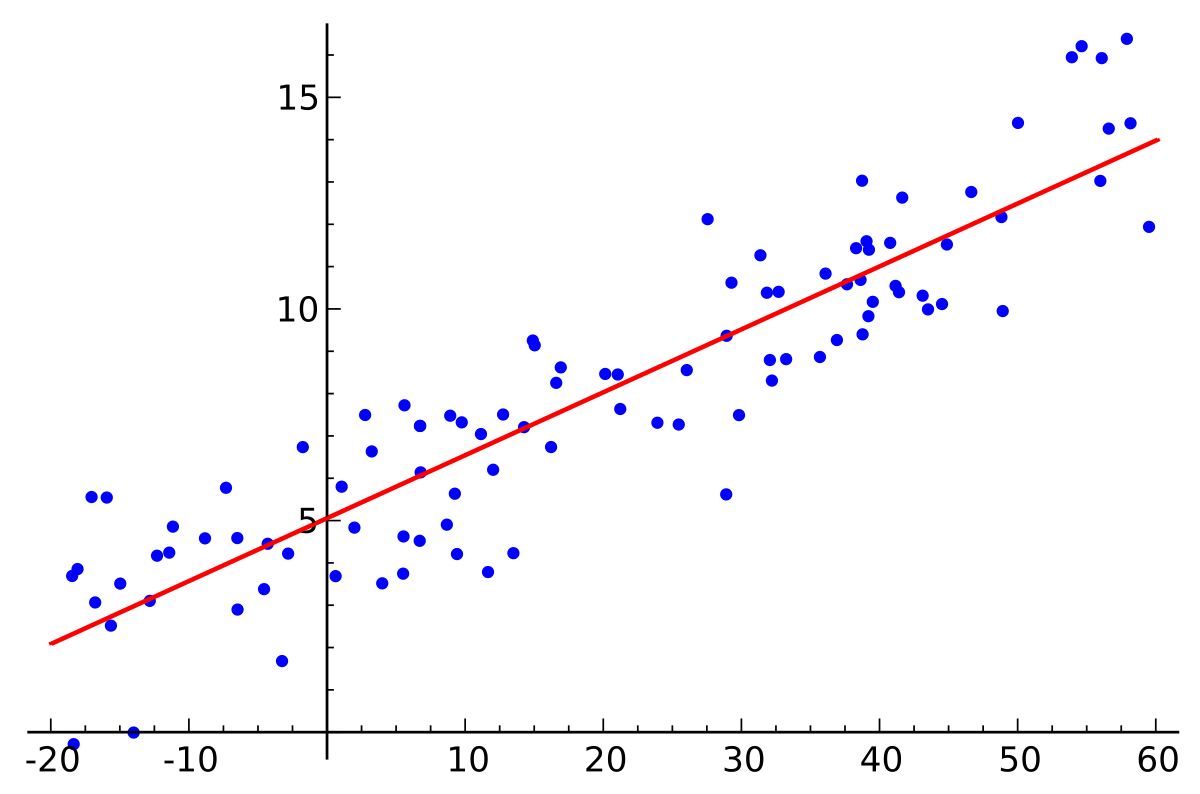
\includegraphics[width=0.45\textwidth]{images_0/linearegre.png}    
\end{center}

The intercept term $b$ is often called the \textbf{bias} parameter, given the fact that the output of the transformation is biased towards $b$ in absence of any input.

\subsection{Capacity, Overfitting and Underfitting}
The central challenge of any machine learning algorithm is to be able to perform well on unseen inputs. The ability to perform well on previously unobserved input is called \textbf{generalization}.

Typically, we training a machine learning algorithm, we can compute some error measure over some training set, the \textbf{training error}, trying to reduce this error; this is simply an optimization problem. What separates machine learning from optimization is that we want to minimize also the \textbf{generalization error}, also called \textbf{test error}. The generalization error is defined as \textit{the expected value of the error on a new input}. When tuning the weights of a machine learning algorithm, we try to find those parameters that minimize the training error, so the test error will generally be greater or equal than the train error. The factors the determine how well an algorithm performs are its ability to:
\begin{itemize}
    \item make the training error small;
    \item make the gap between training and test error small.
\end{itemize}
This correspond to two of the central challenges of machine learning: \textbf{underfitting} and \textbf{overfitting}. The first one occurs when our algorithm is not able to obtain a sufficiently small error value on the training set; the latter occurs when the gap between training and test error is too large.

We can control wheter a model is more likely to overfit or underfit by altering its \textbf{capacity}, which can be informally defined as the ability to fit a wide variety of functions. Models with low capacity may struggle to fit the training set, while models with high capacity tend to overfit by memorizing properties of the training set that do not serve on the test set. One way to control the capacity is by choosing the appropriate \textbf{hypothesis space}, the set of functions that can be chosen by the learning algorithm as being the solution. For example, for linear regression we can generalize to include also polynomials of higher degree, this will increase the model capacity. In general, machine learning algorithms will perform well when their capacity is appropriate to the true complexity of the task that they need to perform and the size of the training data they are provided with.
\section{From Perceptrons to Feed Forward Neural Networks}
Guardati le slides per la prima parte.

\subsection{A Note on Maximum Likelihood Estimation}
The goal of \textbf{Maximum Likelihood} estimation is to make inferences about the population that is most likely to have generated the sample.
Maximum likelihood estimation is a method of estimating the parameters of a probability distribution by maximizing a likelihood function, so that under the assumed statistical model the observed data is most probable. The main appeal of this method derives from the fact that it can be shown to be the best estimator asymptotically (as the number of examples $m \to \infty$) in terms of its rate of convergence as $m$ increases. Under appropriate conditions, as the number of samples goes to infinity, the maximum likelihood estimate of a parameter converges to the true value of a parameter; this property is called \textit{consistency}. 

Let's observe independent identically distributed samples from a Gaussian distribution with known $\sigma^2$:
\begin{center}
    $x_{1}, x_{2}, \ldots, x_{N} \sim N\left(\mu, \sigma^{2}\right) \quad p\left(x | \mu, \sigma^{2}\right)=\frac{1}{\sqrt{2 \pi} \sigma} e^{-\frac{(x-\mu)^{2}}{2 \sigma^{2}}}$  
\end{center}
Let $\theta = (\theta_1,...,\theta_p)^T$ a vector of parameters, we want to find the MLE for $\theta$; we do the following:
\begin{itemize}
    \item write the likelihood $L=P(Data|\theta)$ for the data;
    \item take the logarithm of the likelihood $l=logP(Data|\theta)$, which is called the \textbf{log-likelihood}; this has several advantages, for example for a numerical point of view the product is more prone to underflow;
    \item find the maximum solving $\frac{\partial l}{\partial\theta_i}=0$.
\end{itemize}
The likelihood of the data can be expressed as follows:
\begin{center}
    $L(\mu)=p\left(x_{1}, x_{2}, \ldots, x_{N} | \mu, \sigma^{2}\right)=\prod_{n=1}^{N} p\left(x_{n} | \mu, \sigma^{2}\right)$
$=\prod_{n=1}^{N} \frac{1}{\sqrt{2 \pi} \sigma} e^{\frac{\left(x_{n}-\mu\right)^{2}}{2 \sigma^{2}}}$   
\end{center}
We can transform the product in a sum by taking the logarithm, having the log-likelihood:
\begin{center}
    $\begin{aligned} l(\mu)=\log \left(\prod_{n=1}^{N} \frac{1}{\sqrt{2 \cdot \pi} \sigma} e^{-\frac{\left(x_{n}-\mu\right)^{2}}{2 \cdot \sigma^{2}}}\right)=& \sum_{n=1}^{N} \log \frac{1}{\sqrt{2 \cdot \pi} \sigma} e^{-\frac{\left(x_{n}-\mu\right)^{2}}{2 \cdot \sigma^{2}}}=\\ &=N \cdot \log \frac{1}{\sqrt{2 \cdot \pi} \sigma}-\frac{1}{2 \cdot \sigma^{2}} \sum_{n}^{N}\left(x_{n}-\mu\right)^{2} \end{aligned}$   
\end{center}
Find out the derivative, noting that the first part does not depend on $\mu$:
\begin{center}
    $\frac{\partial l(\mu)}{\partial \mu}=\frac{\partial}{\partial \mu}\left(N \cdot \log \frac{1}{\sqrt{2 \pi} \sigma}-\frac{1}{2 \sigma^{2}} \sum_{n}^{N}\left(x_{n}-\mu\right)^{2}\right)=$
$=-\frac{1}{2 \sigma^{2}} \frac{\partial}{\partial \mu} \sum_{n}^{N}\left(x_{n}-\mu\right)^{2}=-\frac{1}{2 \sigma^{2}} \sum_{n}^{N} 2\left(x_{n}-\mu\right)$
\end{center}
Solve the set of simultaneous equations $\frac{\partial l}{\partial\theta_i}=0$:
\begin{center}
    $-\frac{1}{2 \sigma^{2}} \sum_{n}^{N} 2\left(x_{n}-\mu\right)=0$ \\ $\sum_{n}^{N}\left(x_{n}-\mu\right)=0$ \\
    $\sum_{n}^{N} x_{n}=\sum_{n}^{N} \mu $ \\
    \vspace{0.5cm}
    $\mu^{M L E}=\frac{1}{N} \sum_{n}^{N} x_{n}$
\end{center}
As we can see, the $\mu^{MLE}$ is the average of the $x_n$, so the sample mean is an estimate of the mean and this comes from the fact that you are doing a maximum likelihood estimation of the mean of a Gaussian distribution. This is an unbiased estimator, so it's a nice estimator and we'd like to do the same with neural networks.

\subsection{Neural Networks for Regression}
You want to find the weights so that this network approximates some target value.
\begin{center}
    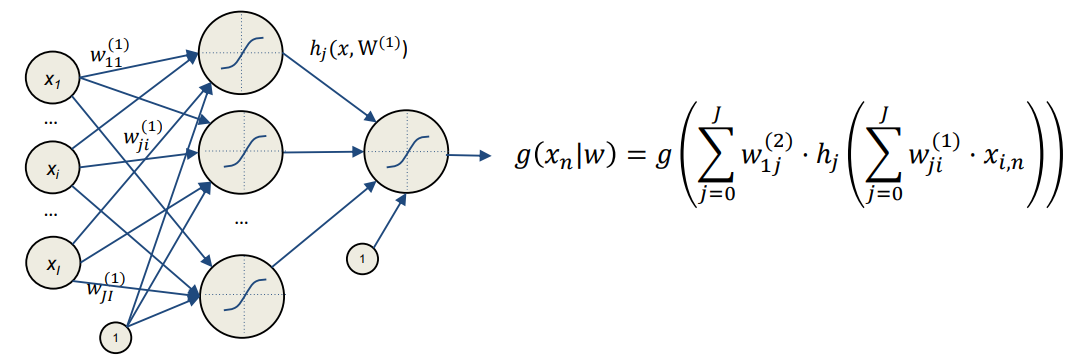
\includegraphics[width=0.8\textwidth]{images_1/per6.png}    
\end{center}
Let's assume $\textbf{t}$ as the function we want to approximate with $N$ observations.
\begin{center}
    $t_{n}=g\left(x_{n} | w\right)+\epsilon_{n}, \quad \epsilon_{n} \sim N\left(0, \sigma^{2}\right)$ 
\end{center}
Let's assume that this network is so good for some weights that besides some noise it is exactly equal to the function 
%(slide 41)
; so let's assume that this data really comes from this network but has been corrupted by noise. I assume that the difference between the prediction and the target is an error which comes from a Gaussian distribution with some noise; this is one possible assumption, we'll take this. We will approximate $t$ as:
\begin{center}
    $t_n \sim N(g(x_n|w),\sigma^2)$
\end{center}
So we have i.i.d samples coming from a Gaussian distribution as follows:
\begin{center}
    $t_n \sim N(g(x_n|w),\sigma^2)$
    
    $p(t|g(x|w),\sigma^2)=\frac{1}{\sqrt{2\pi}\sigma}e^{-\frac{(t-g(|w))^2}{2\sigma^2}}$
\end{center}
Let's try to compute the maximum likelihood %of the mean 
as a function of the weights, which are our parameters. The likelihood is the joint probability of all the observations [in case of a Gaussian distribution]: 
$$
L(w)=p(t_1, t_2, ..., t_N | g(x|w), \sigma^2)=\prod_{n=1}^{N} p\left(t_{n} |g\left(x_{n} | w\right), \sigma^{2}\right)=
\prod_{n=1}^{N} \frac{1}{\sqrt{2 \pi} \sigma} e^{-\frac{\left(t_{n}-g\left(x_{n} | w\right)\right)^{2}}{2 \sigma^{2}}}
$$
%we need to know the likelihood of the data which is for a Gaussian the joint probability of all the observations, which means the product of the observations:
Look for the weights which maximize the likelihood: 
\begin{center}
    $\operatorname{argmax}_{w} L(w)=\operatorname{argmax}_{w} \prod_{n=1}^{N} \frac{1}{\sqrt{2 \pi} \sigma} e^{-\frac{\left(t_{n}-g\left(x_{n} | w\right)\right)^{2}}{2 \sigma^{2}}}$
\end{center}
These are the canonic Gaussian but the mean is replaced with $g\left(x_{n} | w\right)$, which means a function parametrized in a given set of parameters $w$ evaluated in x. You want to compute the maximum of the likelihood; instead of product we can take the logarithm:
$$
\operatorname{argmax}_{w} \sum_{n}^{N} \log \left(\frac{1}{\sqrt{2 \pi} \sigma} e^{-\frac{\left(t_{n}-g\left(x_{n} | w\right)\right)^{2}}{2 \sigma^{2}}}\right)=\operatorname{argmax}_{n} \sum_{n}^{N} \log \frac{1}{\sqrt{2 \pi} \sigma}-\frac{1}{2 \sigma^{2}}\left(t_{n}-g\left(x_{n} | w\right)\right)^2
$$
We can see that $-\frac{1}{2 \sigma^{2}}$ is a negative constant so we have to remove it by changing the sign of this function: instead of maximize we have to minimize. The max likelihood weights are obtained by minimizing this:
\begin{center}
    $ \operatorname{argmin}_{w} \sum_{n}^{N}\left(t_{n}-g\left(x_{n} | w\right)\right)^{2} $
\end{center}
%So the keypoint of using the sum of squares errors is that you are assuming this; under this assumptions finding the weights that minimize the sum of squares errors means to estimate the weights with the max like approach. 
What if our error does not come from a Gaussian distribution? If the error is not a Gaussian distribution, you can still do this but it's not the best solution and it's not a maximum likelihood estimation so you might end up with a solution that is not unbiased (unbiased means an estimator with zero bias). 
But if you know that the errors are distributed differently you can follow the process and you will get the exact solution. 

\subsection{Neural Networks for Classification}
Let's start with a very well known problem: \textit{Classification}. Let's talk about binary classification: the output is either 0 or 1
%, so the output of the network can only be distributed as a distribution that outputs 0 or 1.
Let's assume our model now estimates the probability of class 1, instead of the class 0, for example using a sigmoid function. We can assume that the target comes from a Bernoulli distribution and the network is basically estimating what is the probability of 1 (or 0, equally). 
\begin{center}
    $g\left(x_{n} | w\right)=p\left(t_{n} | x_{n}\right), \quad t_{n} \in\{0,1\} \quad$ 
    $t_{n} \sim B e\left(g\left(x_{n} | w\right)\right)$
\end{center}
So when you are training this network you are basically training a classifier which predicts the a-posteriori probability of a class. We can write:
\begin{center}
    $t_{n} \sim B e\left(g\left(x_{n} | w\right)\right) \quad p\left(t|g(x | w))=g(x | w)^{t} \cdot(1-g(x | w))^{1-t}\right.$
\end{center}
So the probability of getting a $t=1$ is $g(x | w)^{t}$ and  $(1-g(x | w))^{1-t}$ if $t=0$. \\
$t$ acts as a \textit{selector}. The likelihood is the following, assuming that the samples are i.i.d:
\begin{center}
    $\begin{aligned} L(w)=& p\left.(t_{1}, t_{2}, \ldots, t_{N}|g(x | w))=\prod_{n=1}^{N} p\left(t_{n}\left|g\left(x_{n} | w\right)\right)=\right.\right.\\ &=\prod_{n=1}^{N} g\left(x_{n} | w\right)^{t_{n}} \cdot\left(1-g\left(x_{n} | w\right)\right)^{1-t_{n}} \end{aligned}$
\end{center}
We want to maximize the likelihood and once again we take the sum of logarithms:
\begin{center}
    $\operatorname{argmax}_{w} L(w)=\operatorname{argmax}_{w} \prod_{n=1}^{N} g\left(x_{n} | w\right)^{t_{n}} \cdot\left(1-g\left(x_{n} | w\right)\right)^{1-t_{n}}$
    $=\operatorname{argmin}_{w}-\sum_{n}^{N} t_{n} \log g\left(x_{n} | w\right)+\left(1-t_{n}\right) \log \left(1-g\left(x_{n} | w\right)\right)$
\end{center}
We minimize instead of maximizing and what we get is really different from the sum of squares, this is our error function:
\begin{center}
    $E(w)=-\sum_{n}^{N} t_{n} \log g\left(x_{n} | w\right)+\left(1-t_{n}\right) \log \left(1-g\left(x_{n} | w\right)\right)$
\end{center}
This error is called \textbf{Binary Cross-Entropy}:
minimizing this is very different from minimizing the sum of squares error because they solve two different problems,  Regression vs Classification, additive Gaussian noise vs predictive Bernoulli distribution. The key aspect is that the error function that you are minimizing is describing the problem to the network. Basically nowadays many papers on "how to learn something" are describing the error functions. 

We have discussed the binary classification problem but this can be written also for multi-class problems. The error is called \textbf{Cross-Entropy}. \\

\begin{wrapfigure}{r}{6cm}
    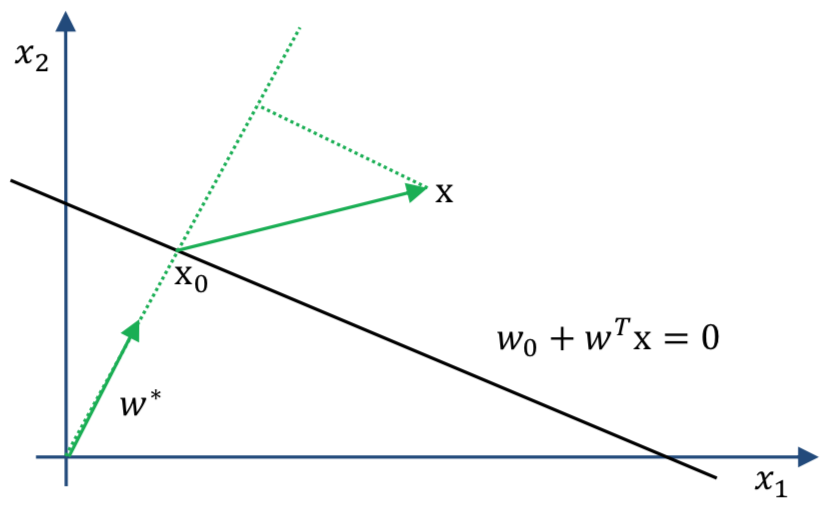
\includegraphics[width=6cm]{images/perceptron_decbound.png}
\end{wrapfigure} 

If you consider perceptron, is there any implicit cost in the perceptron rule? To understand this we need a little bit of math. \\
%Perceptron are more or less lines. 
Let's consider the hyperplane (affine set) $\boldsymbol{L \in \mathbb{R}^2}$ [the decision boundary of the perceptron]:
%(min 13:43 reg 3, slide 49)

\begin{center}
    $L: w_{0}+w^{T} x=0$
\end{center}
Let's think about our problem in a 2-dim space: the perceptron is deciding between a +1 or a -1. For any two points $\mathrm{x}_{1}$ and $\mathrm{x}_{1}$ on $\boldsymbol{L \in \mathbb{R}^2}$, it means that $w_0 + w^T \mathrm{x}_{1}=0$ and $w_0 + w^T \mathrm{x}_{2}=0$. We have that the \textit{normal vector} of $\mathrm{x}_{1} - \mathrm{x}_{2}$ (which specify the direction of the hyperplane $\boldsymbol{L}$) is $w^T$, in fact:
\begin{center}
    $w^{T}\left(\mathrm{x}_{1}-\mathrm{x}_{2}\right)=0$
\end{center}
%$\mathrm{x}_{1}$ is a point and you can think as a vector going from the origin to that point (slide 49), $\mathrm{x}_{2}$ is the other vector; so $\mathrm{x}_{1}-\mathrm{x}_{1}$ is the other vector (la differenza tra i due). 

The \textit{versor normal} to $\boldsymbol{L \in \mathbb{R}^2}$ is then: $ w^* = \frac{w}{||w||}$. For any point $x_0$ in $\boldsymbol{L \in \mathbb{R}^2}$ we have:
$$
w^{T} x_{0}+w_{0}=0 \rightarrow
w^T x_0 = -w_0
$$
$w$ is something like $(\mathrm{w}_{1},\mathrm{w}_{2})$ so it's a vector as well. \\
%When does the product between the two vectors become equal to zero? As always, when they are orthogonal, so you can interpret $w$ as an orthogonal vector to the decision boundary. If you want to normalize you can just divide by the norm, obtaining the versor $w^{*}=w /\|w\|$ which is the normal normal to my decision boundary. For any point $x_{0}$ on the line, being on the line means that $w^{T} x_{0}+w_{0}=0$, so $w^{T} x_{0}=-w_{0}$. 
%There is this nice property: you take the equation of the line you compute at any point in space and divide by the norm of the weights, this is the distance of this point from the line itself::
Taking any point $\boldsymbol{x}$ in $\mathbb{R}^2$ and considering the difference vector of $\boldsymbol{x} - \mathrm{x}_{0}$, the projection on the direction of $W^*$ of that vector is: 
$$
w^{*T} (\boldsymbol{x} - \mathrm{x}_{0}) = \frac{w^T}{||w||} (\boldsymbol{x} - \mathrm{x}_{0}) = \frac{1}{||w||} w^T(\boldsymbol{x} - \mathrm{x}_{0}) = \frac{1}{||w||} (w^T\boldsymbol{x} - w^{T}\mathrm{x}_{0}) = \frac{1}{||w||} (w^T\boldsymbol{x} + w_0)
$$
where $w^{*T} (\boldsymbol{x} - \mathrm{x}_{0})$ corresponds to the distance of x from the hyperplane $\boldsymbol{L}$ [the projection], so $(w^T\boldsymbol{x} + w_0)$ is proportional to the distance of $\boldsymbol{x}$ from the plane defined by $(w^T\mathrm{x} + w_0)=0$ [$\boldsymbol{L}$].\\
To sum up, the previous procedure means that the distance of a point $\boldsymbol{x}$ from the hyperplane (i.e. the projection of $(\boldsymbol{x} - \mathrm{x}_{0})$ on the direction of $w^*$, the normal versor of the hyperplane) is \textit{equal} to $(w^T\boldsymbol{x} + w_0)$ multiplied by a scalar factor $\frac{1}{||w||}$.\\
%Basically this term is proportional to the distance of $x$ from the plane defined by $\left(w^{T} x+w_{0}\right)=0$. 
If the vector is above the line, the distance is positive; if the vector is below the line then the distance is negative. \\

\textit{Perceptron Learning Algorithm} The output of the perceptron can be +1/-1:
\begin{itemize}
    \item If an output $t=+1$ is misclassified (your prediction is $t=-1$), then $\left(w^{T} x+w_{0}\right) < 0$
    \item On the other side if the output is $t=-1$ and your prediction is $t=+1$, then $\left(w^{T} x+w_{0}\right) > 0$
\end{itemize}{}

%that means that errors can be of two types:
%\begin{itemize}
%    \item +1 but $\left(w^{T} x+w_{0}\right)<0$;
%    \item -1 but $\left(w^{T} x+w_{0}\right)>0$.
%\end{itemize}

We can see that in errors the product of the two (classification label and $\left(w^{T} x+w_{0}\right)$) is always negative, so we can write this error which tries to minimize the product between the target and the distance of a misclassified point $x_i$ from the hyperplane:
%(which is the perceptron boundary, as we just shown):
\begin{center}
    $D\left(w, w_{0}\right)=-\sum_{i \in M} t_{i}\left(w^{T} x_{i}+w_{0}\right)$
\end{center}
%Basically if you have an error you want to minimize the product of $t_{i}$ and the distance; 
where $M$ is the set of misclassified points. \\

%To minimize this we could compute it for all errors and then simply doing stochastic gradient descend, this is the batch approach. On other option is just doing stochastic gradient descent on each single error, so it's the stochastic gradient descent of this error function. Gradient descent w.r.t. the model parameters is:
Minimizing by stochastic gradient descent the error function $d(w,w_0)$, the gradients with respect to the model parameters are:
\begin{center}
    $\frac{\partial D\left(w, w_{0}\right)}{\partial w}=-\sum_{i \in M} t_{i} \cdot x_{i} \quad \frac{\partial D\left(w, w_{0}\right)}{\partial w_{0}}=-\sum_{i \in M} t_{i}$
\end{center}
Stochastic gradient descent applies for each misclassified point:
\begin{center}
    $\left(\begin{array}{l}{w^{k+1}} \\ {w_{0}^{k+1}}\end{array}\right)=\left(\begin{array}{l}{w^{k}} \\ {w_{0}^{k}}\end{array}\right)+\eta\left(\begin{array}{c}{t_{i} \cdot x_{i}} \\ {t_{i}}\end{array}\right)$
\end{center}
This is exactly Hebbian Learning:
%, and this came after Hebbian Learning and they did not know that. This is the right thing to do: 
model the error as the distance of points wrongly classified from the boundary. This is different because it does not say anything about probabilities. The perceptron is a classical \textit{discriminative} approach, on the contrary feed forward neural network trained with cross-entropy is a classical \textit{generative} approach (generative methods try to predict some a-posteriori probability, discriminative approaches instead don't care at all of probabilities, they just take a line).

Anyways this latter thing is not used anymore because you need to do this update for each misclassified point and it could be very long.
%, but it's just to show that you can have several error functions and error functions describe a problem, and even the perceptron was performing in a way a minimization problem via backpropagation. 

These error functions are nowadays called \textbf{Loss Functions}. The term loss actually comes from stochastic risk minimization, where you want to minimize the risk and integrate the loss over all possible outcomes etc., but for us it's something that you want to minimize. How do I design error functions? You can use the knowledge about the data distribution or you can have some background information (cross-entropy and perceptron are built in different ways in this sense) or finally, you can use your creativity.
% Feedforward neural networks and Backpropagation ?
% Error Functions ?
\section{Image Classification}
\textbf{Computer Vision} is an interdisciplinary scientific field that deals with how computers can be made to gain \textbf{high-level understanding} from digital images or videos. \\
The connection between Computer Vision and Machine Learning is undergoing a dramatic change: once, most of techniques and algorithms were built upon a mathematical/statistical description of images. Nowadays, machine-learning methods are much more popular: you don't need anymore to go to all these mathematical/statistical models, but you just let a network to resolve a defined task. \\
In case of Classification, the input is an \textbf{image} which corresponds to a set of pixels each associated to a \textit{set of colors}: in each pixel in a colored image you can get three different values (Red, Green, Blue), so we can consider three different images. Videos are sequence of images (frames), so if a frame is $ I \in \mathbb{R}^{R \times C \times 3} $ where 3 represents the RGB values, a video of $T$ frames is defined as
$$
V \in \mathbb{R}^{R \times C \times 3 \times T}
$$
The fourth dimensions is the frame number in the sequence. \\
Dimensions is terribly increasing: a pixel is 1 byte, so without compression a single frame in full HD is stored with $6MB$. Fortunately, visual data are very redundant, thus compressible. A picture is saved in jpeg, which is a lossless compression algorithm that transform the input in a different domain where it can be better compressed. \\

\subsection{Local (Spatial) Transformations}
The simplest operation on an image is a \textit{local transformation} which can be written as $$ G(r,c) = T_U[I(r,c)]
$$
where
\begin{itemize}
    \item I is the input image to be transformed
    \item G is the output
    \item $T_U: \mathbb{R}^3 \rightarrow \mathbb{R}^3$ or  $T_U: \mathbb{R}^3 \rightarrow \mathbb{R}$ is a function
    \item $U$ is neighbourhood, identifies a region of the image that will concur in the output definition
\end{itemize}{}
$T$ operates on $I$ "around" $U$. $T$ can be either linear or nonlinear.\\

\begin{wrapfigure}{r}{5cm}
    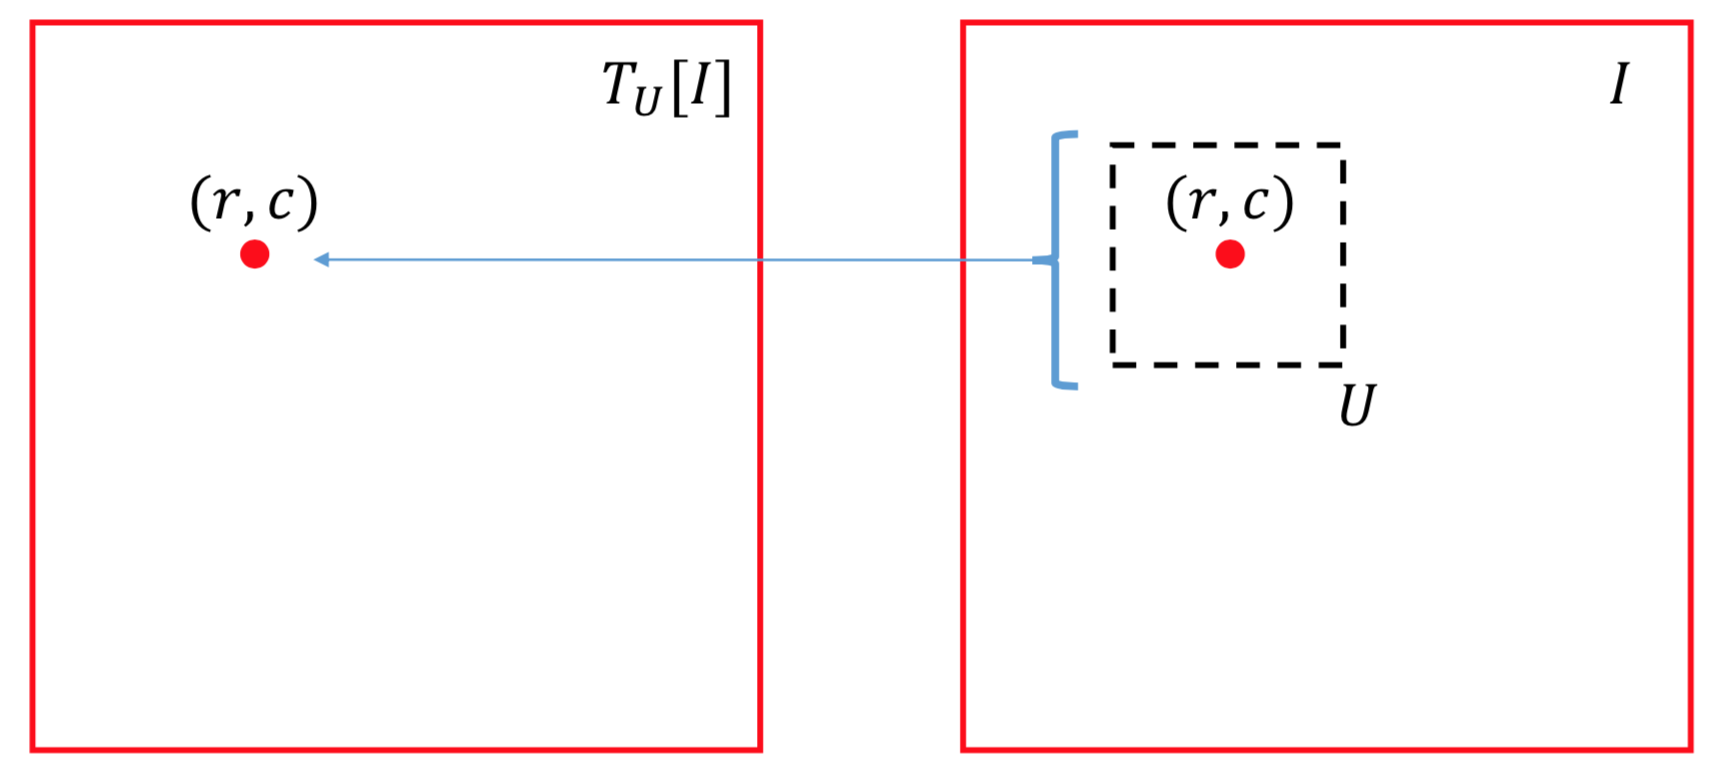
\includegraphics[width=5cm]{images/local_transformation.png}
\end{wrapfigure} 

\textbf{Filter Transformation} takes around each pixel a suitable neighbourhood and defines the output of the transformation by looking only on those values here around.  The output of a filter is a sort of function defined in a neighbour of a pixel. \\
The simplest one is the \textbf{Linear Transformation}: given a pixel, the output of the filter in that pixel is provided by a linear combination of the pixel around that pixel. The output is the linear combination of the weights and the intensity of the values. 
$$ T(I(r,c)) = \sum_{(x, y) \in U} w_i * I(r+x, c+y) = \sum_{(x, y) \in U} w(x, y) * I(r+x, c+y) $$
The parameters of that operation are the weights $w_i$: they can be written like an image, in a matrix. The weights now are arranged in a matrix are called \textbf{Filter $h$}: the filter $h$  entirely defines this operation. This is the Linear Filtering: \\
\begin{minipage}{\linewidth}
        \centering
        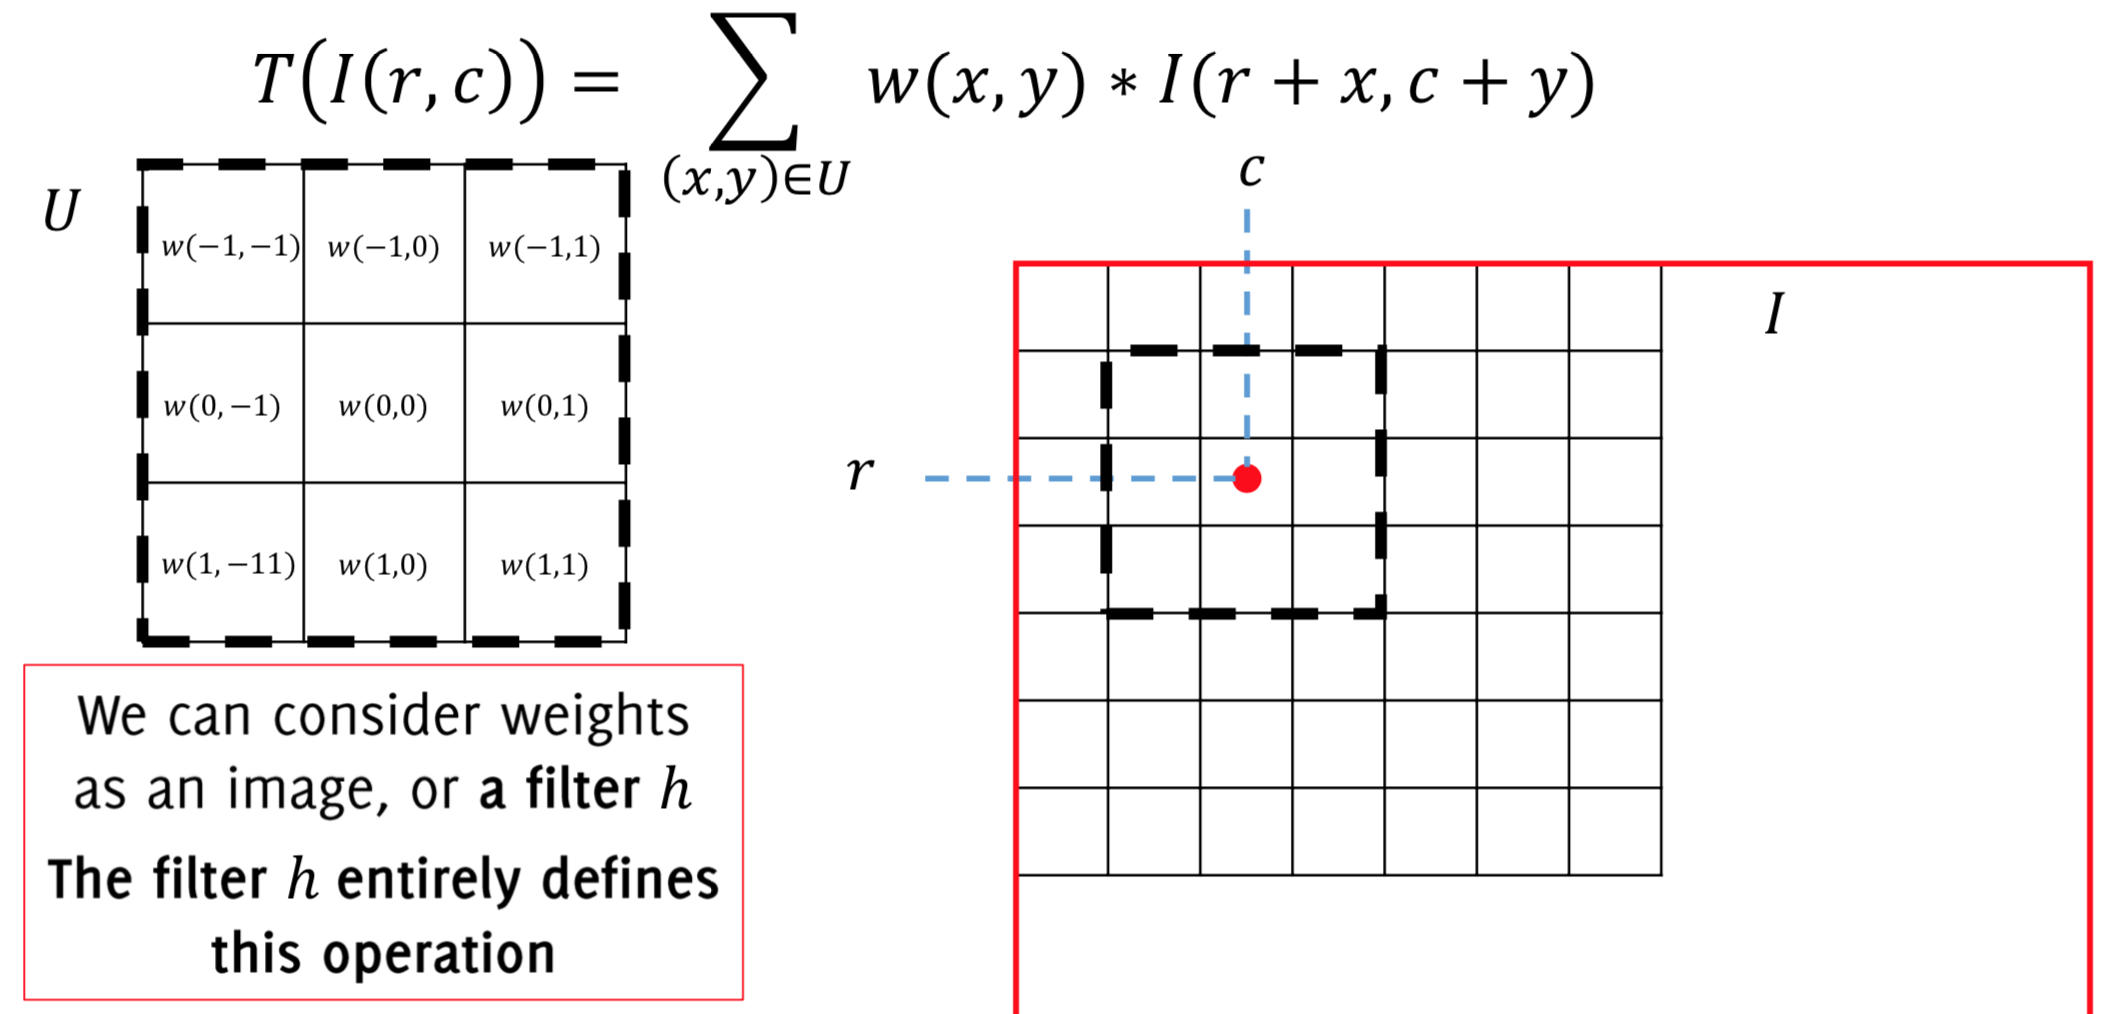
\includegraphics[width=9cm, height=5cm]{images/linear_filter.png}
        %\captionof{figure}{Logical Architecture}
        \label{fig:log_arch}
\end{minipage} \\

The \textbf{Correlation} among a filter $h$ and an image is defined as 
$$
(I \otimes h)=\sum_{u=-L}^{L} \sum_{v=-L}^{L} h(u, v) * I(r+u, c+v)
$$
where the filter $h$ is of size $(2L+1) * (2L+1)$. 
The idea is that you take a filter and 
you overlap it 
%it is like overlapping this filter 
to each location of the image. This operation is performed on each color of the image. \\
"UTK" correlated with "T" example - slide 48: \\
The weights of the filters are 0 or 1 (black or white), when I put the filter over the T in the image, I get the number of pixels equal to 1 in the T. The zeros next to the T is higher, as you move slightly about of the T the intensity of the output increasing since there will be some zeros that will overlap to the T. In this way we can compare images or I can use it to find where the T is in my image. It is enough to know where the T is by taking the local maxima in the correlation output. What you get is where the Ts are. Sometimes we need some sort of normalization to get the things works. 

\subsection{Problem Definitions}
There are different problems to which we focus on:
\begin{itemize}
    \item \textbf{Image Classification}: Assign to an input image $I$ a label $l$ from a fixed set of categories: the classifier gives you the probabilities over each class. $$I \rightarrow l$$
    \item \textbf{Localization}: Assign to an input image $I$ a label $l$ from a fixed set of categories and the coordinates $(x, y, h, w)$ of the bounding box enclosing that object. $$I \rightarrow (x, y, h, w,l)$$
    \item \textbf{Object Detection}: Assign to an input image $I$ \textbf{multiple} labels $\{l_i\}$ from a fixed set of categories, each corresponding to an \textbf{instance of that object}, and the coordinates $\{(x, y, h, w)_i\}$ of the bounding box enclosing \textbf{each} object. 
    $$
    I \rightarrow\left\{(x, y, h, w, l)_{1}, \dots,(x, y, h, w, l)_{N}\right\}
    $$
    \item \textbf{Image Segmentation}: Assign to \textbf{each pixel} of an input image $I$ a label $\{l_i\}$ from a fixed set of categories $\Lambda$ $$ I \rightarrow S(x,y)$$ where $S(x,y) \in \Lambda$. The output of segmentation is an image itself.
    \item \textbf{Instance Segmentation}: Assign to an input image $I$ \textbf{multiple} labels $\{l_i\}$ from a fixed set of categories $\Lambda$, each corresponding to an \textbf{instance of that object}, the coordinates $\{(x, y, h, w)_i\}$ of the \textbf{bounding box enclosing each object}, the \textbf{set of pixels} in each bounding box corresponding to that label 
    $$
    I \rightarrow\left\{(x, y, h, w, l,S)_{1}, \dots,(x, y, h, w, l,S)_{N}\right\}
    $$
    It is like a mix between object detection and segmentation because for each input image you have to assign multiple labels, each one corresponding to instance of an object, to each object you have to provide a bounding box and there is a list of pixel inside the bounding box covered by the object. You can distinguish different persons, in segmentation you cannot.

\end{itemize}
Is this a \textit{challenging problem}? 
\begin{enumerate}
    \item Images are very \textbf{high-dimensional data}.
    \item \textbf{Label Ambiguity}: a label might not uniquely identify the image.
    \item \textbf{Transformation}: you can perform an image transformation that does not change the content, the meaning of the image, but changes the intensity values of the image, so the pixel values.
    \item \textbf{Inter-class Variability}: images belonging to the same class can be dramatically different. 
    \item \textbf{Perceptual Similarity}: it's not pixel-wise similarity, but it means the way you perceive two images to be similar.
\end{enumerate}{}
%We focus on image classification problem. 
%(Esempio su Nearest Neighbourhood Classifier pag.82: you measure the distance between two vector. In case of images you can perform pixel-wise distance among images. \\
%The pixel-wise similarity (the one in the NN-classifier) would not be successful on image. The pixel-wise similarity does not understand the perceptual similarity.) \\

\subsection{Nearest Neighborhood Classifier}
Assign to each test image, the label of the \textbf{closest image} in the training set: 
$$
\hat{y}_{j}=y_{j^{*}}, \quad \text { being } j^{*}=\underset{i=1 \ldots N}{\operatorname{argmin}} d\left(x_{j}, x_{i}\right)
$$
Distances are typically measured as: 
\(d\left(x_{j}, x_{i}\right)=\left\|x_{j}-x_{i}\right\|_{2}=\sqrt{\sum_{k}\left(\left[x_{j}\right]_{k}-\left[x_{i}\right]_{k}\right)^{2}}\)
 
You are measured the distance between two vectors, so basically you are computing a \textit{pixel-wise similarity}. \\
In the same way you can create a K-Nearest Neighborhood Classifier which assigns to each test image, the most frequent label among the \textbf{K-closest} images in the training set. \\
Both the methods will not work since the pixel-wise similarity does not \textit{understand} the perceptual similarity. \\
Pros: 
\begin{itemize}
    \item Easy to understand and implement
    \item It takes no training time
\end{itemize}{}
Cons: 
\begin{itemize}
    \item Computationally demanding at test time
    \item Large training set have to be stored in memory
    \item Rarely practical on images: distances on high-dimensional objects are difficult to interpret
\end{itemize}{}

\subsection{Linear Classifier}
A classifier can be seen as a function that maps an image $x$ to a confidence score for each of the $L$ classes: $$\kappa: \mathbb{R}^d \rightarrow \mathbb{R}^L $$
where $\kappa(x)$ is a $L$-dimensional vector and the i-th component $s_i = [\kappa(x)]_i$. A good classifier associates to the correct class a score that is larger than the scores associated to incorrect classes. \\
Dealing with images, the input \textbf{x} belongs to $\mathbb{R}^d$ where $d$ is the dimension of the image. The Linear Classifier get an input image and extract a set of scores for each class, but need to be linear. In Linear Classification, $\kappa$ is a \textbf{linear function}: 
$$ \kappa(x) = Wx + b $$
where $W \in \mathbb{R}^{L \times d}$ are the weights , $b \in \mathbb{R}^L$ is the bias, both are the parameters of the classifier. \\ 

\begin{minipage}{\linewidth}
        \centering
        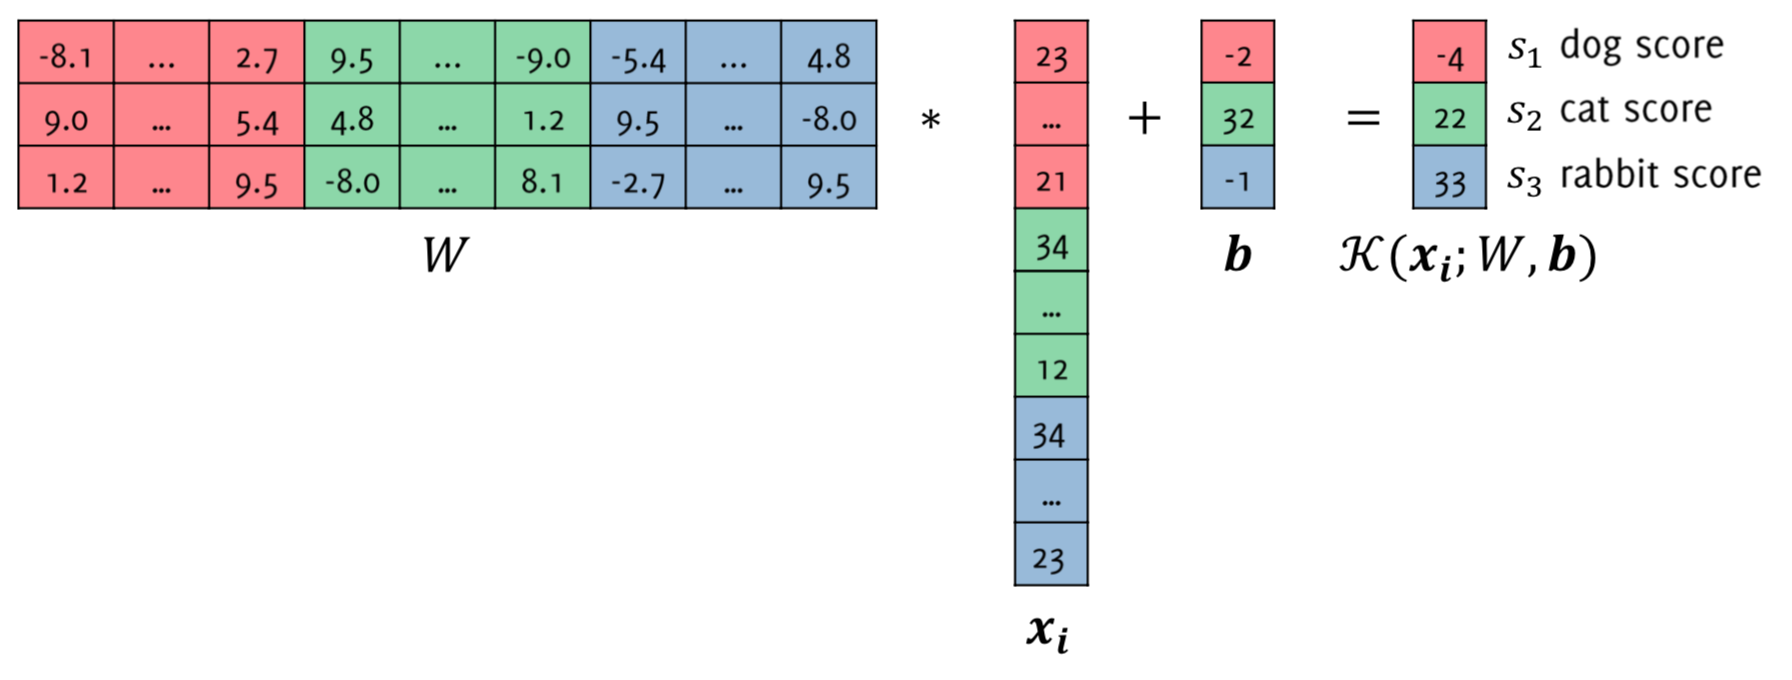
\includegraphics[width=12cm, height=5cm]{images/linear_class.png}
\end{minipage}

So you need to perform a linear transformation of the input vector and what you obtain as output is a vector in which each component is the score assigned to each class. In the \textit{weights matrix}, each row corresponds to the weights related to a class; a row has the same size $d$ of the input image vector $x_i$. To create the input image vector, starting from an image (and from the red image of an RGB), you unroll it column-wise: from top-left corner, you read column wise and move from red to green to blue images. 
%and you start all the red pixel in the top part of your vector, then you move to the green and at the end to the blue part. 
This corresponds to your vector $x_i$, your input image i. So the linear classifier operation is row (a class) times column (your input), which output is a vector of L values, one for each class. Adding the bias we get the last output of the classifier as results. The classifier assign to an input image the class corresponding to the largest score 
$$
\hat{y}_{j}=\underset{i=1, \ldots, L}{\operatorname{argmax}}\left[s_{j}\right]_{i}
$$
The parameters of this classifier are the weights, so we need to train this classifier in order to learn the weights: weights indicate which are the most important pixels / colors. Also the value of bias is in your parameters. The number of parameters are $d \times L + L$, which are the exactly number of parameter in a layer of a neural network. \\
Given a training set and a loss function, define the parameters that minimize the loss function over the whole training set, so in case of linear classifier: 
$$
[W, b]=\operatorname{argmin}_{W \in \mathbb{R}^{L \times d}, b \in \mathbb{R}^{L}} \sum_{\left(x_{i}, y_{i}\right) \in T R} \mathcal{L}\left(\boldsymbol{x}, y_{i}\right)+\lambda \mathcal{R}(W, b)
$$
The loss function has to be regularized to achieve a unique solution satisfying some desired property, where $\lambda > 0$ is a parameter balancing the two terms. \\ 
\subsubsection{Geometric Interpretation of a Linear Classifier}
Given a classifier already trained with $W$ and $b$. The first intuition, if you take the matrix $W$ and input $x$, you can add the bias and compute the scores. What contribute to the scores of the first class is just the first row of the matrix. So you can see the i-th row of $W$ as the classifier corresponding to the i-th class. It just a matter of computing a inner product between $w_i$ and an input $x$.\\
%(pag 106)
If we were in two-dimension, an image is like a point, each row of the matrix identifies that linear function which corresponds to a set of (hyper-)plane where if the input point is above or below that plane it means that the point belongs or not to a class. So what you are doing is looking at your image in a $d$-dimensional space and trying to separate classes by hyper-plane and dividing your input images by 'putting' them in one of these hyper-planes. \\ \\
\textit{Geometric interpretation}: you take an high-dimensional space, try to separate images through hyper-planes and you define the hyper-plane in order to do the best you can do for the given training set. \\

Another interpretation: taking $W$, a row of $W$ contains $d$ values which is the same size as image, so we can reshape it to generate an image and visualize it like an image $\rightarrow$  Template. So you multiply this template for your input and sum the bias for each template and this is exactly correlation that we have seen before. The Linear Classifier is just learning some template to which it performs correlation against and you provide as output the class of the template that provides you the largest response. 
\section{Training and Overfitting}
\begin{quote}
    \textit{"A single hidden layer feedforward neural network with S shaped activation functions can approximate any measurable function to any desired degree of accuracy on a compact set"} \\
    \textbf{Universal approximation theorem (Kurt Hornik, 1991)}
\end{quote}

The universal approximation is good if you want a non-linear function approximator, you can use feed-forward neural network and you can learn anything but there are some drawbacks: 
\begin{itemize}
    \item[--] It doesn’t mean we can find the necessary weights: it may be difficult to learn everything, since it is not easy to find out the starting point and be sure to converge on the right place. There is a place in parameter space where your network approximate your function perfectly, but it is up to you to find this place.
    
    \item[--] An exponential number of hidden units may be required: it is true that this object can approximate everything but the point is that it may require an infinite/exponential number of hidden neurons, so it may be impractical to do it.
    
    \item[--] It might be useless in practice if it does not generalize: it can perfectly fit the data but it might not follow the original function $\rightarrow$ \textbf{Overfitting}: a model has learned to provide good performance at training time but it is not able to perform (to generalize) properly at testing time. 
\end{itemize}{}

 If you think to the problem of learning a continue function, let's assume you have a set of samples and  you have a network that is over complex, so you can incur in a situation like the one represented in the right part of Fig.\ref{fig:model_complexity}. The problem is when you get new data, those data may be close to the function, but it does not mean that the function that I have learned is closed to those data [since the predicted function is over complex]. 
 
 \begin{figure}[h]
    \centering
    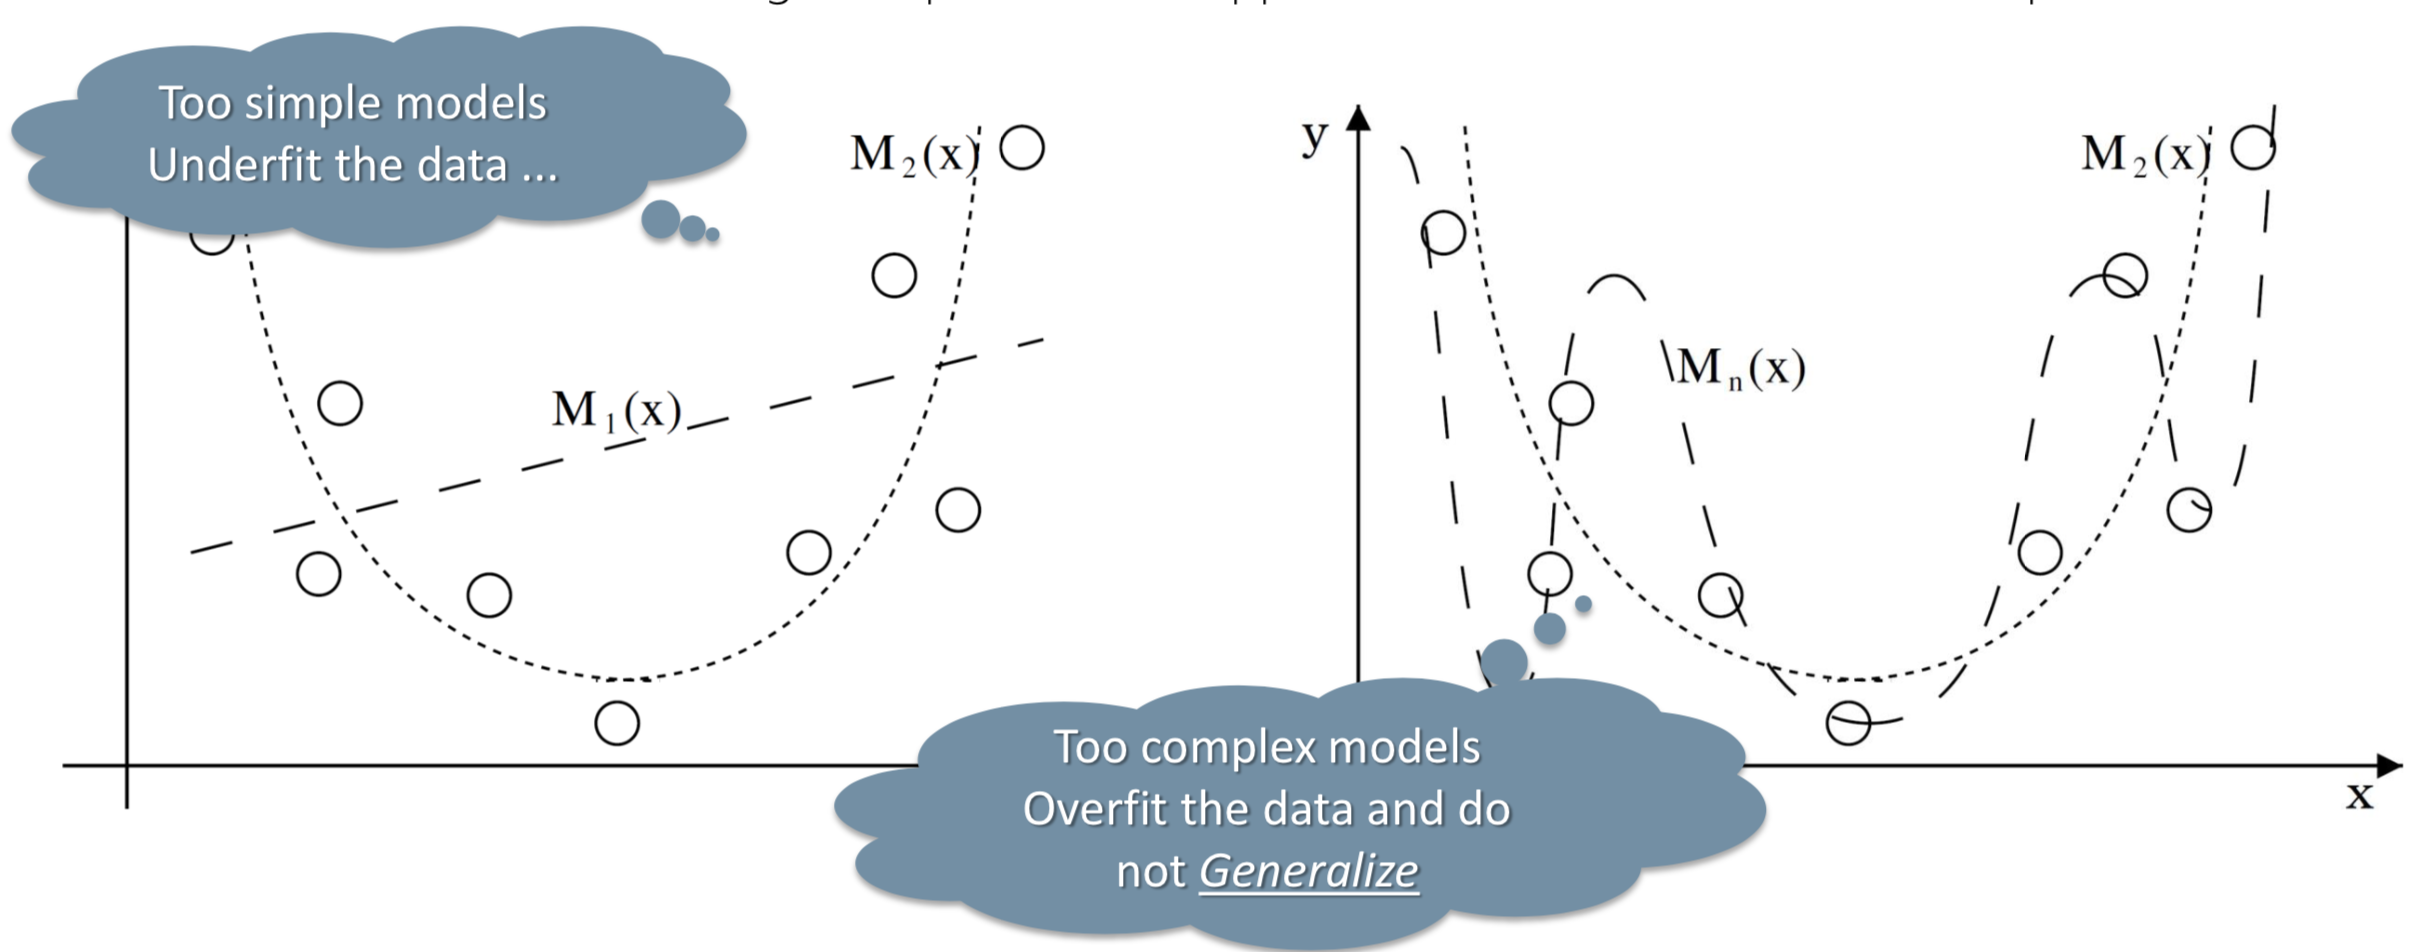
\includegraphics[width=15cm, height=6cm]{images/model_complexity.png}
    \caption{Under-fitting \& Over-fitting}
    \label{fig:model_complexity}
\end{figure}

 In fact, you tried to minimize the error on the train, but you lost the ability to generalize over new data: the model is not able to Generalize. It is an old story called Ockham's Razor: \textit{between a simple model and a very complex one you have to chose always the simple one}.\\
 In the other hand we have \textbf{Underfitting} when the model is too simple w.r.t. the real model. Too complex model tends to overfitting, so very good performance in training but very low performance in testing. You need to prevent overfitting.\\
 We need to find a way to measure the \textbf{Generalization}: training error/loss is not a good indicator of performance on future data:
 \begin{itemize}
     \item[--] The model has been learned from the very same training data, any estimate based on that data will be optimistic
     \item[--] New data will probably not be exactly the same as training data
    \item[--] You can find patterns even in random data
 \end{itemize}{}
 
 The idea is that you cannot use the same data of the training; you require a new independent set of data. Usually you take the data and split them in two sets: we train on one set and we test on the other. We \textit{never ever} use the test set at training time. Sometimes you can \textit{sample} the data \textit{with replacing}: it means that there is some probability for the same data to be in test and in train. This random sampling with replacing is called \textbf{Bootstrap} and it is used when the dataset is very small. What is important is that you want the training data to have the same distribution of your test data; what is done is \textbf{Stratified Sampling}: by doing it, essentially you are doing Cross Validation. The latter can have different form: hold-out set (but you have to be lucky to get a set that reflect the test set. With a small dataset, it could be problematic because the performance on test-set will depend on the separation taken into account), leave-one-out (not feasible for a huge amount of data), k-fold cross validation (averaging the performance of each fold).
 
 \subsection{Dealing with Overfitting}
Some of the strategies to deal with overfitting in neural network are presented in the following section:

\subsubsection{Early Stopping: Limiting Overfitting by Cross-Validation}
This is the most effective one if you have enough data. 
The point is that if you monitor the error on unseen data (validation-set) during the training process, you will reach a point in which your model has the minimum error on those new data. Once found this point, you can stop the training and consider it as the best model. To do this you need another set of data besides train and test: splitting the train-set, you get another train-set and a validation-set. The test set is used as the last thing to estimate the model on new data. The validation set is used during the training. You never use the validation to learn but only to stop the learning procedure.\\
To recap, \textit{Overfitting} networks show a \textbf{monotone} [decreasing] training error trend (on average
with SGD) as the number of gradient descent iterations \textbf{k}, but they lose generalization at some point, so we need to:
\begin{itemize}
    \item Hold out some data
    \item Train on the training set
    \item Perform cross-validation on the hold out set
    \item Stop train when validation error increases
\end{itemize}{}

One tipical procedure that is used to set up the neurons is to evaluate early stopping (the generalization error) to decide on other parameters, since the validation set error is an estimate of the error that you will get on test set. This idea of deciding on the parameters of the network is called \textbf{Hyper-parameter tuning}. Hyper-parameter describe the network structure and, once defined it, you know how many parameter you have to optimize. 

\subsubsection{Weights Regularization}
Sometimes you don't want to remove some data because you would like to exploit all of them. So there are technique to prevent overfitting without stopping the model, but instead somehow limiting the capability of the complex model: we have a powerful model but we impose some constraint on the model \textit{freedom}, based on a-priori assumption. \\
In case of neural network, we need to introduce a concept based on Bayesian Statistics: so far we have seen the problem of learning a model as a maximum learning estimation problem. We have been estimated the parameters of model in order to maximize the \textit{likelihood} of the data. What we show now is the difference between \textit{Frequentist} approach and \textit{Bayesian} approach. If we take the coin toss, the Frequentist approach bases the probabilities on the number of times I hit head/cross over the total number of tosses. The Bayesian approach has an opinion on the probabilities of head based on a bias (initially bias means that we assume that the coin is balanced, so we have 50\% head/cross); I toss the coin and I see head: the frequentist said that the prob. of head is $1$. The bayesian instead said $0.5$, one toss it is not enough to change the opinion. Second toss, second head: frequentiest said prob. of head is 1; bayesian said is not enough. After 10000 toss and 10000 heads the bayesian changes opinion. \\

According to the \underline{frequentist} approach, you have \underline{no opinion}: you look to the data and you select among all possible model the one that fits better the data $\rightarrow$ Unfortunately, this is basic overfitting, because you cannot bias the model. \\

On the other hand, the \underline{bayesian} approach starts from \underline{an opinion} that have a great \underline{bias}, and this prevent bayesianist to change opinion because he have seen only few data. \\

In statistics, opinions are named \textit{priors}. Maximum likelihood estimation finds the weights which maximize the data probability. A bayesianist looks for the most probable weights: in this way we are looking for \textbf{maximum a-posteriori}, we look for the most probable weights having observed data. The main difference between this two is that one looks for the probability of the data given the weights and the other for probability of the weights given the data. Substantially it is the \textbf{Bayes theorem}: $$
\begin{aligned}
w_{M A P} &=\operatorname{argmax}_{w} P(w | D) \\
&=\operatorname{argmax}_{w} P(D | w) \cdot P(w)
\end{aligned}
$$
This formula give you the possibility to bias the weights: i.e. if for you any weight is the same, this probability is uniform and you get maximum likelihood estimation because there is no difference between one and the other; if you want a model which is smooth, you have to put a prior probability which act as smoothy factor. \\
The idea of maximum a-posteriori is to force the model to select some weights and not other. It's sort of forcing, not a constraint. \\

How we define the prior in a way that our network does not overfit? It is observed in practice that \textit{small weights} makes network less prone to overfit; the bigger the weights the more likely the network overfit. Basically what we would like to do is limiting the capability of changing w.r.t. the variation on the input. \\
But what is that a small variation in the input become big in the output? The weights: they are the parameters, so they control the magnitude of the model.  That's why in general networks with small weights overfit less. We need to force our algorithm to prefer small weights: to do it, one possible way is to say that if you take all the weights, on average they have to be as small as possible, so near to zero on average. Then the bigger they become, the less likely they become. \\

One possible way to enforce bias on the weight distribution is to ask for the weight distribution as a Gaussian with zero-mean and some variance $\sigma_w^2$. \\
Instead of maximize likelihood we want to maximize a-posteriori probability, so we maximize the probability of the weights given the data. Let's assume we are in regression setting and the probabilities of weights are:
$$
P(w) \sim N\left(0, \sigma_{w}^{2}\right)
$$
$$
P(w) =  \frac{1}{\sqrt{2 \pi} \sigma_{w}} e^{-\frac{\left(w_{q}\right)^{2}}{2 \sigma_{w}^{2}}}
$$

Assume that $Q$ is the number of weights on the network (includes all the parameters in the network): 

$$
\begin{aligned}
\widehat{w} &=\operatorname{argmax}_{w} P(w | D)=\operatorname{argmax}_{w} P(D | w) P(w) \\
&=\operatorname{argmax}_{w} \prod_{n=1}^{N} \frac{1}{\sqrt{2 \pi} \sigma} e^{-\frac{\left(t_{n}-g\left(x_{n} | w\right)\right)^{2}}{2 \sigma^{2}}} \prod_{q=1}^{Q} \frac{1}{\sqrt{2 \pi} \sigma_{w}} e^{-\frac{\left(w_{q}\right)^{2}}{2 \sigma_{w}^{2}}} \\
&=\operatorname{argmin}_{w} \sum_{n=1}^{N} \frac{\left(t_{n}-g\left(x_{n} | w\right)\right)^{2}}{2 \sigma^{2}}+\sum_{q=1}^{Q} \frac{\left(w_{q}\right)^{2}}{2 \sigma_{w}^{2}} \\
&=\operatorname{argmin}_{w} \sum_{n=1}^{N}\left(t_{n}-g\left(x_{n} | w\right)\right)^{2}+\gamma \sum_{q=1}^{Q}\left(w_{q}\right)^{2}
\end{aligned}
$$

Where we define $\gamma = {\sigma^2 \over \sigma_w^2}$

The regularization term is positive. Adding a regularization term you are less prone to overfit because it makes your model smooth. \\
To force the network to have small weights we have to minimize the fit of the data plus some regularization term that is the sum of the squared of the weights $\rightarrow$ Ridge regression in Regression model does exactly this.\\ 
This is a classical form of loss function, another one is to add the sum of the absolute values of the weights $\rightarrow$ Lasso: it brings some weight to zero. \\

The best $\gamma$ is the one that minimize the generalization error: we can use Cross-Validation to select the proper $\gamma$. \\
In neural network literature, this approach that uses quadratic regularization term in error function is called \textbf{Weight Decay}. 





\subsubsection{Dropout}
By turning off randomly some neurons we force to learn an independent feature preventing hidden units to rely on other units (co-adaptation): each hidden unit is set to zero with $\boldsymbol{p_j^{(l)}}$ probability, e.g. $\boldsymbol{p_j^{(l)}} = 0.3$. \\
\textbf{Dropout} trains weaker classifiers, on different mini-batches and then at test time we implicitly average the responses of all ensemble members. At testing time we remove masks and average output (by weight scaling). \\
This technique modifies the network itself, not its loss function. It removes a small percentage of neurons on each hidden layer, chosen randomly.\\
It behaves as an ensemble method: it's like we have an ensemble of a lot of different networks. \\

\begin{minipage}{\linewidth}
        \centering
        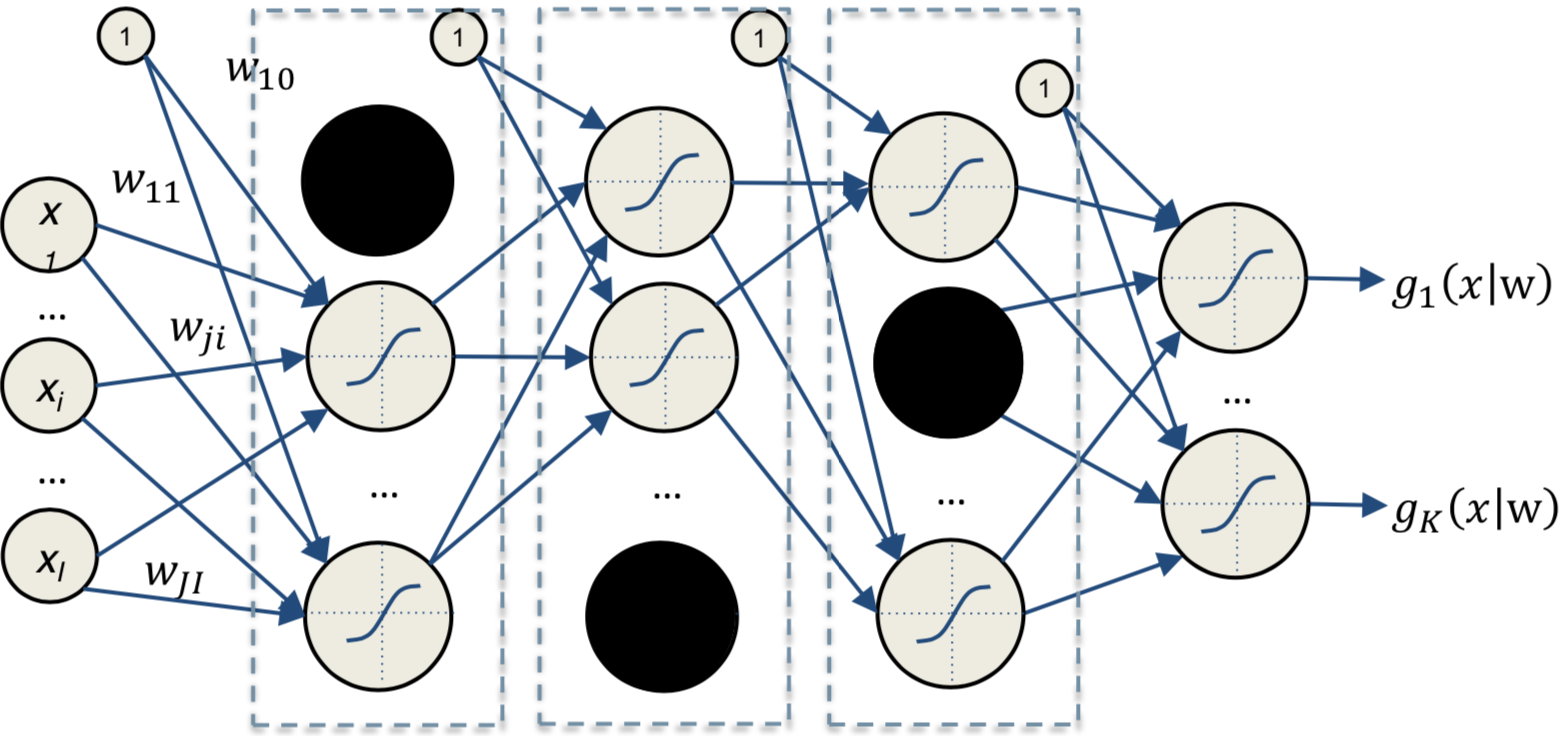
\includegraphics[width=13cm, height=5cm]{images/dropout.png}
        %\captionof{figure}{Logical Architecture}
        \label{fig:log_arch}
\end{minipage}\\



\subsection{Tips and Tricks}
Activation functions such as Sigmoid or Tanh saturate, which leads to:
\begin{itemize}
    \item[--] Gradient is close to zero
    \item[--] Backpropagation requires gradient multiplication
    \item[--] Gradient faraway from the output vanishes
    \item[--] Learning in deep networks does not happen
\end{itemize}{}

The problem of \textbf{Vanishing Gradient} raises from the fact that when you have very complex long neural network, to compute the gradient, you have to compute all the chain of derivatives:
$$
\frac{\left.\partial E\left(w_{j i}^{(1)}\right)\right)}{\partial w_{j i}^{(1)}}=-2 \sum_{n}^{N}\left(t_{n}-g_{1}\left(x_{n}, w\right)\right) \cdot g_{1}^{\prime}\left(x_{n}, w\right) \cdot w_{1 j}^{(2)} \cdot h_{j}^{\prime}\left(\sum_{j=0}^{J} w_{j i}^{(1)} \cdot x_{i, n}\right) \cdot x_{i}
$$
In deep networks, the gradient results in a very small number. \\
The issue is in Sigmoidal and Hyperbolic Tangent functions since the maximum of the derivative is in the origin and if we define they as a function $g()$, we know that 
\begin{itemize}
    \item for Sigmoid: $g'(a) = g(a)(1-g(a))$ $\rightarrow$ the maximum of the derivative is where the values is 0.5, so the maximum is equal to $0.5 (1 - 0.5) = 0.25$
    \item for Tanh: $g'(a) = 1 - g(a)^2$
\end{itemize}{}

In general the derivative is less than 1. The main issue with gradient descent is that the only way to fix it is by changing the operator function, so we need to use activation functions that do not suffer of this issue of having the derivative less than 1 $\Rightarrow$ \textbf{ReLU}

\subsubsection{ReLU}
\begin{wrapfigure}{r}{4cm}
    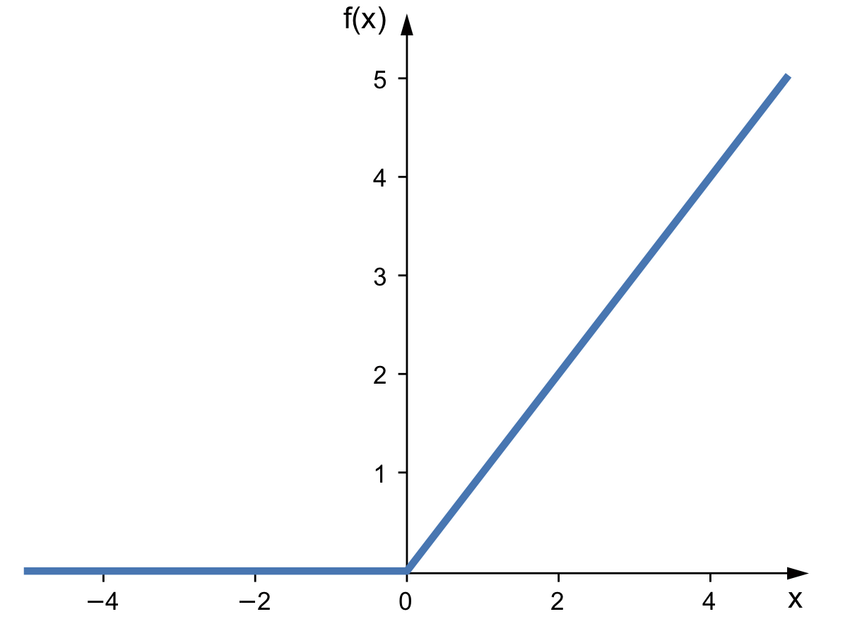
\includegraphics[width=5cm]{images/relu.png}
    %\label{fig:lstm_org}
\end{wrapfigure}  

The ReLU (Rectified Linear Unit) activation function is defined as:

$$ 
g(a) = ReLu(a) = max(0,a) 
$$ 

$$
g^{\prime (a)} = 1_{a>0}
$$ \\ \\

and it has some interesting properties:
\begin{itemize}
    \item[--] The derivative is either 1 or 0. Compute the derivative is essentially an "if"
    \item[--] Faster SGD Convergence: in the backward chaining, once you get the zero, you can forget about the past
    \item[--] Sparse activation (only part of hidden units are activated):  if on average half of the activation functions will be positive and the other half negative, then half of these neuron are switched off, so we don't have to compute it. Increase the efficiency and increase generalization since function is more simple, so it is more likely to not overfit.
    \item[--] Efficient gradient propagation (no vanishing or exploding gradient problems): you multiply by 1 or 0. 
    \item[--] Efficient computation (just thresholding at zero)
    \item[--] Scale-invariant: $max(0,a = a max(0,x)$. To some extent it is more robust to conditions, it is not affected by the values of current activation functions. 
    \item[--] It is not a linear function. 
\end{itemize}{}

But also potential disadvantages:
\begin{itemize}
    \item[--] Non-differentiable at zero: however it is differentiable (so not a significant issue)
    \item[--] Non-zero centered output: if you want the model outputs a number that is not strictly positive, you can use it. If you want a strictly positive output, you have to use a linear activation function.
    \item[--] Unbounded: Could potentially blow up
    \item[--] \textit{Dying Neurons}: ReLU neurons can sometimes be pushed into states in which they become inactive for essentially all inputs. No gradients flow backward through the neuron, and so the neuron becomes stuck and "dies", no way of switching it on. It decrease the model capacity and usually happens with high learning rates
\end{itemize}{}

Dying Neurons is an issue, but in the other hand switching off some neuron it's good since we create a simpler model. The problem is when it happens too early, i.e. at initialization time. Another thing that could happen: sometimes having a big learning rate could generate issues with these neurons because they become inactive too early w.r.t. training time.

%the derivative of g ... (guardare appunti dopo dropout). 
%Multiplying these number results in a very small number. The issue is in sigmoidal function or hyperbolic tangent since the maximum of the derivative is in the origin and if we define it as $g$, we know that for the sigmoid $g'(a) = g(a)(1-g(a))$, the maximum of the derivative is where the values is 0.5, so the maximum is equal to $0.5 (1 - 0.5) = 0.25$ [This is the maximum value]. In case of tanh the derivative is $g'(a) = 1 - g(a)^2$. So in general the derivative is less than 1. The main issue with gradient descent is that the only way to fix it is by changing the operator function. So we need to use activation functions that do not suffer of this issue of having the derivative less than 1 --> RELU: it has interisting properties: 
%\begin{itemize}
    %\item The derivative is 1: so the gradient are all either 1 o 0. So compute the derivative is an 'if'
    %\item Is not a linear function. 
    %\item In the backward chaining, once you get the zero, you can forget about the past (?) --> it is faster to compute with relu
    %\item You end up on sparse activation: if on average half of the activation function will be positive and the other half negative, on average half of these neuron are switched off, so we don't have to compute it. Increase the efficiency and increase generalization since function is more simple, so it is more likely to not overfit.
    %\item Efficient gradient propagation since there is no vanishing gradient and no exploding (it means when the derivative is greater than 1): in fact if you multiply number greater than 1, this number grows and grows and explodes resulting on unstable results. 
    %\item It is scale gradient, to some extent it is more robust to conditions, it is not affected by the values of current activation functions. 
%\end{itemize}{}

%Disadvantages:
%\begin{itemize}
%    \item It is not differentiable on zero: this is not significant issue
%    \item Non-zero centered output: if you want the model outputs a number that is not strictly positive, you can use it. If you want a strictly positive output, you have to use a linear activation function
%    \item It is unbounded: because of numerical optimization, it could grows unbounded
%    \item Dying neurons: the true issue. If you have the gradient equal to zero means that it will never change the weight. So if for some reason the gradient of this weight becomes zero, there will be no way of changing its weights, so there is no way to switch on this neuron. It is an issue, but in the other hand switching off some neuron it's good since we create a simpler model. The problem is when it happens too early, i.e. at inizialization time. Another thing that could happen: sometimes having a big learning rate could generate issues with these neurons because they become inactive too early wrt training time
%\end{itemize}{}

The main solutions are: 
\begin{itemize}
    \item Leaky RELU: the negative part decreases slowly, so there is a small gradient and when you go near or less than 0, you have a little chance to come back/to recover instead of switching itself off. It fix the "dying ReLU" \\
    \vspace{0.2cm}
    \begin{minipage}{\linewidth}
        \centering
        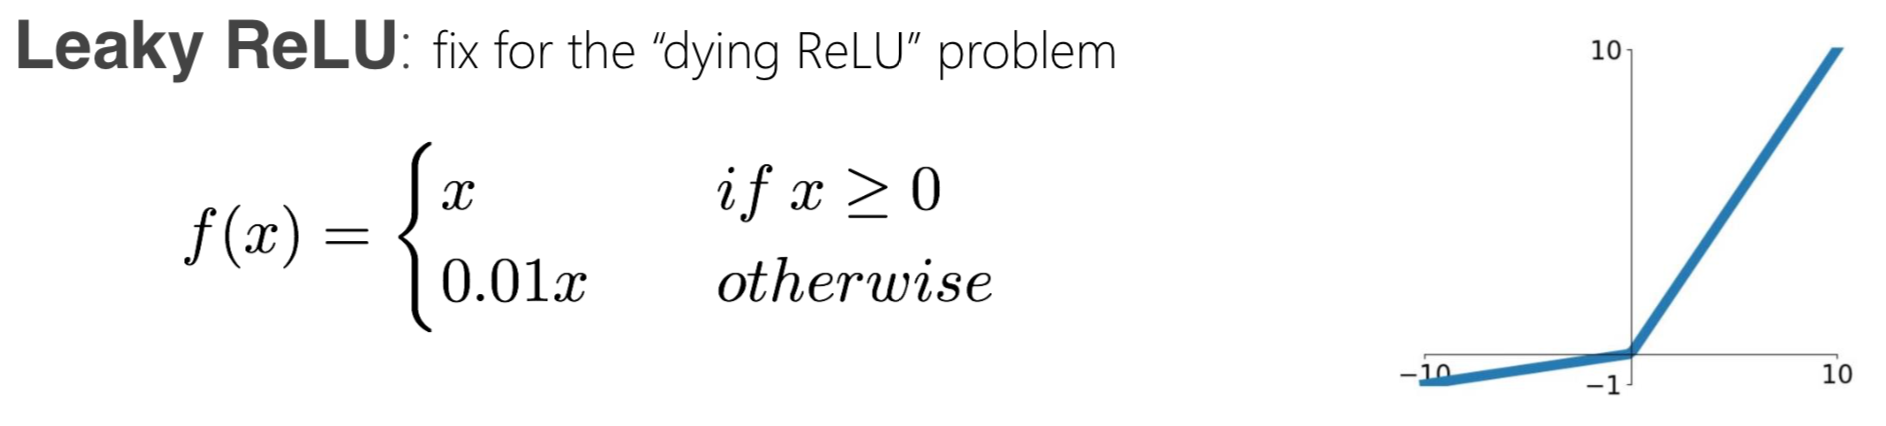
\includegraphics[width=14cm, height=3.5cm]{images/leaky_relu.png}
        %\captionof{figure}{The model pipeline.}
        %\label{fig:flow_fig}
    \end{minipage}

    \item ELU: you have an exponential and a lineal part and you can tune the $\alpha$ for the exponential part to define how much you would like to go under zero. It tries to make the mean activations closer to zero which speeds up learning. $\alpha$ hand by hand \\
    \vspace{0.2cm}
    \begin{minipage}{\linewidth}
        \centering
        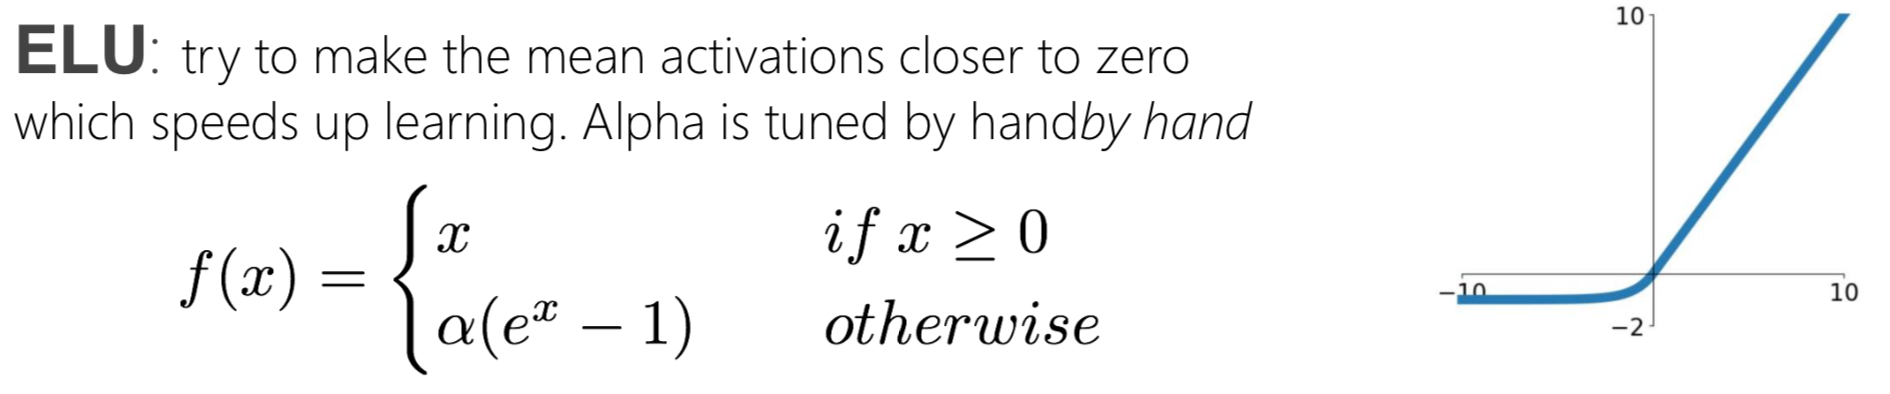
\includegraphics[width=14cm, height=3.5cm]{images/elu.png}
        %\captionof{figure}{The model pipeline.}
        %\label{fig:flow_fig}
    \end{minipage}
    
\end{itemize}{}

Modern architectures use ReLU, since initialization is a problem per-se.

\subsubsection{Weights Inizialization}
The final result of gradient descent is affected by weight initialization:
\begin{itemize}
    \item \textit{Zero}: it does not work. All gradient would be zero, no learning will happen. 
    \item \textit{Big Numbers}: bad idea. Assume to use sigmoid function and very big weights , you are in an area which gradient is close to zero $\rightarrow$ Long-time to converge
    \item \textit{Classic strategy}: small weights sampled by Gaussian distribution with zero mean and low variance. It works decently. The bigger is the variance the more it takes to training, since the weights are big and they are big when there are on the wrong side, so they take more time. Small number are fine: the weights starts more or less with the maximum of the gradient $\rightarrow$ at the very beginning the learning is fast. It is good for small networks, but it might be a problem for deeper neural networks.
\end{itemize}{}

However, in deep networks:
\begin{itemize}
    \item In a big network, if the weights are too small, you get the shrink gradient, since the gradient is the product of derivatives but also of the weights along a path. The gradient will not be zero but will be very small
    \item If you start with large weights, the gradient grows as it passes through the layers and at certain point will be too big. Assume you have a fixed learning rate, since in a way you tune the weights as (weight - learning rate * gradient), if the gradient grows, the product grows, so you have huge change in the weights. 
\end{itemize}{}

Some proposal to solve the problem is \textbf{Xavier Initialization}: \\
Suppose we have an input $x$ with $I$ components and a linear neuron with random weights $w$. The output of this neuron is
$$
h_{j}=w_{j 1} x_{1}+\cdots+w_{j i} x_{I}+\cdots+w_{j I} x_{I}
$$
We can derive that $w_{ji}x_{i}$ is going to have variance:
$$
\operatorname{Var}\left(w_{j i} x_{i}\right)=E\left[x_{i}\right]^{2} \operatorname{Var}\left(w_{j i}\right)+E\left[w_{j i}\right]^{2} \operatorname{Var}\left(x_{i}\right)+\operatorname{Var}\left(w_{j i}\right) \operatorname{Var}\left(x_{i}\right)
$$
%equal since it is a linear neuron, it is the weighted sum of the input. If you compute the variance of each of this element, what happen is that you are computing the variance of the weights and the input: the variance of weights * input is (formula slides).
Let's assume that both input and weights have zero-mean: 
$$
\operatorname{Var}\left(w_{j i} x_{i}\right)=\operatorname{Var}\left(w_{j i}\right) \operatorname{Var}\left(x_{i}\right)
$$
For the weights it is reasonable; for the input, it is not mandatory, but it has been observe that if you condition the input to have zero-mean and unitary variance, the optimization algorithm is better conditioned and it is more stable. 
%So it turns out that it is a product of variances (formula). 
If we assume all $w_i$ and $x_i$ are \textit{i.i.d} we obtain:
$$
\operatorname{Var}\left(h_{j}\right)=\operatorname{Var}\left(w_{j 1} x_{1}+\cdots+w_{j i} x_{I}+\cdots+w_{j I} x_{I}\right)=n \operatorname{Var}\left(w_{i}\right) \operatorname{Var}\left(x_{i}\right)
$$
So each neuron amplifies the variance of the input by a factor $nVar(w_i)$.\\
Assume that we have unitary variance input, what we don't want to do is to increase the variance of the input too much, so we try to force it to be consistently zero-mean and unitary along all the layers, we should enforce that the gain of the weights on each neuron should be 1: 
$$nVar(w_j) = 1$$
For this reason Xavier proposes to initialize 
$$w \sim N \left( 0,\frac{1}{n_{in}} \right)$$
More fast in converging and more stable.
%Make the assumption that all weigth are iid and all inputs are iid (formule). So each neuron amplifies n*Var(w) the variance of the input. Assume that we have unitary variance input, what we don't want to do is to increase the variance of the input too much, so we try to force to be consistently zero mean and unitary variance along all the layers: to do this we should enforce that the gain of the weights of each neuron should be 1, on average. 
%Spiegazione: assume I have the input and you can see the network as projecting the input in an higher dimensional space where I learn my model. If I make this zero-mean and unitary variance what happens is that at the very beginning I get n*Var(w), and so learning in this space may have conditioning properties, because in that space, weights and numbers are too big. So the fact that you normalize your input, it means that after one layer it explodes, because of this amplified effect on each neuron. To reduce the amplified effect, you want that the variance of the weights for that neuron multiplied by the number of input should be 1: by doing this, on average, what you get after the first layer has still zero-mean and unitary variance and after another layer has still zero-mean and unitary variance. The Xavier initialization propose to initialize the weights of each neuron sampling from a normal distribution with zero mean and a variance equal to 1/number of input [n] --> more fast in converge and more stable during training. 

Glorot and Bengio found a similar result: $n_{out}Var(w_j) = 1$, so they propose: 
$$w \sim N \left( 0,\frac{2}{n_{in} + n_{out}} \right)$$
More recently, He proposed, for rectified linear units:
$$w \sim N \left( 0,\frac{2}{n_{in}} \right)$$

\subsubsection{Momentum}
The idea is to accelerate training and giving to it some inertia.\\

\begin{wrapfigure}{r}{6cm}
    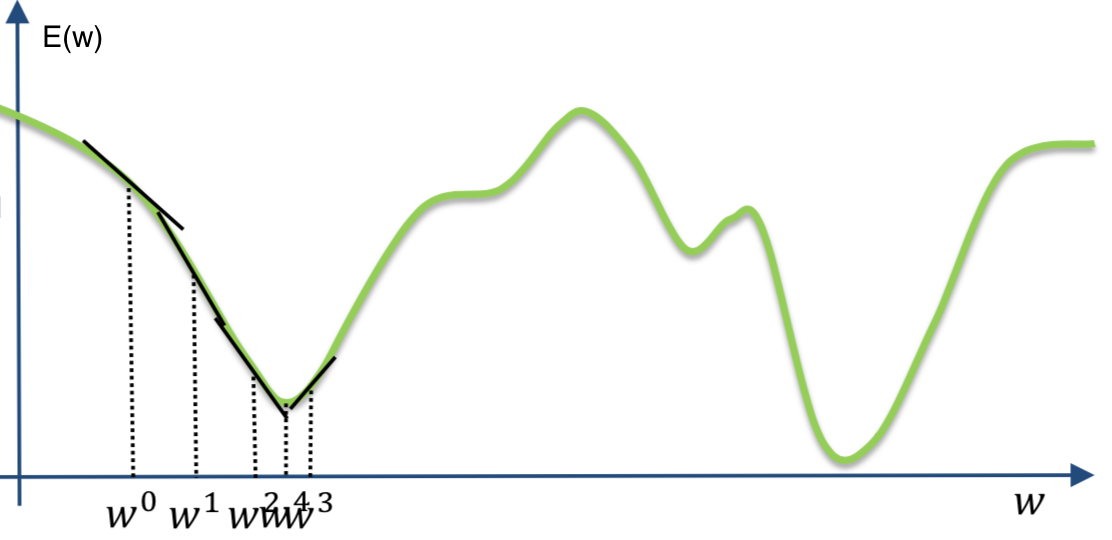
\includegraphics[width=6cm]{images/local_minima.png}
    %\label{fig:lstm_org}
\end{wrapfigure}  

Recalling Backpropagation, finding weights of a Neural Network is a non-linear minimization process: 
$$
\operatorname{argmin}_{w} E(w)=\sum_{n=1}^{N}\left(t_{n}-g\left(x_{n}, w\right)\right)^{2}
$$
We iterate from an initial configuration:
$$
w^{k+1}=w^{k}-\left.\eta \frac{\partial E(w)}{\partial w}\right|_{w^{k}}
$$

To avoid local minima we can use \textbf{Momentum}:
$$
w^{k+1}=w^{k}-\left.\eta \frac{\partial E(w)}{\partial w}\right|_{w^{k}}-\left.\alpha \frac{\partial E(w)}{\partial w}\right|_{w^{k-1}}
$$\\

\textbf{Nesterov Accelerated Gradient} makes a jump as momentum, then adjust
$$
w^{k+\frac{1}{2}}=w^{k}-\left.\alpha \frac{\partial E(w)}{\partial w}\right|_{w^{k-1}}
$$
$$
w^{k+1}=w^{k}-\left.\eta \frac{\partial E(w)}{\partial w}\right|_{w^{k+\frac{1}{2}}}
$$
The Nesterov idea is improving the estimate by dividing in two steps: the first step uses the momentum and it gives you a direction; in the second step re-estimate/update the gradient here, where the momentum leads you.\\
It should be a better estimate since the gradient will be closer to the minimum. It turns out to be more efficient, converges fast than SGD. \\

%There are 2 different algorithm, gradient descent and momentum. 
%\begin{itemize}
%    \item Nesterov Accelarated gradient: if you do standard momentum, you add to the gradient the momentum, so you have a sort of vector addiction which is the momentum. The point is that when you decide to compute the gradient, basically the idea is that you could improve on the estimate by dividing this two in two steps. The momentum gives you a direction where to move, so if you move that direction you will explore piece of error function which could give you more information about the gradient. Nesterov divides in two steps it, in the first half step you apply the momentum, so you move where the momentum lead you; the you re-estimate the gradient there, which should be a better estimate of the gradient closer to the minimum, and you update using the gradient there. It turns out to be more efficient, converge fast than SGD. So the idea is using the previous gradient to provide the better estimate where I should linearize my function. 
%\end{itemize}{}

There are other algorithms that try to \textbf{adapt learning rates} while learning, to deal with:
\begin{itemize}
    \item Gradient magnitudes vary across layers
    \item Early layers get "vanishing gradients": the gradient will be smaller and smaller the more you go back. It means that in the very first layer it should be boosted by an higher learning rate. 
    \item Should ideally use separate adaptive learning rates
\end{itemize}{}

Several algorithm are proposed: Rprop, Adagrad, RMSprop, AdaDelta and many others. \\
How they works? \\
Basically they study the error functions finding a lot of \textit{saddle points}: they are points in where you have two directional derivatives equal to 0, but in one direction it is a minimum, in the other is a maximum. Neural Networks have a lot of these points and having some stochasticity, which means not necessarily going directly to the minimum but having some noise, it will help a lot.

%there are other algorithm that tries to adapt learning rate while learning: the gradient is smaller and smaller the more you go on the back: it means that the information which arrives in the very first layer, should be boosted by the learning rate more at the one at very beginning. Also because the error close to the output, depends on all the error done before, so you should first fix the first weights and then the last one, otherwise you adapt on the error on the input before getting the solution. The idea is that each layer should have its own learning rate: but deciding the learning rate is very difficult in general, and decide it for each layer is impossible. So there are algorithm that adapt the learning rate. It means that the gradient keeps oscillating, it means that the learning rate is too big and you need to reduce it. Some of the algorithms, Adagrad, try to to adapt learning rate though time depending on the speed of convergence of the algorithm. Two most famous algorithm for this are Adagrad and Adam. How it works? (grafico appunti pag 31)
%This error function is called saddle since it contains saddle points: it is a point in where you have two directional derivatives = 0, but there is not the minimum: so in one direction is a minimum, in the other is a maximum. Neural Networks have a lot of these points: having some stochasticity, which means not necessarily going directly to the minimum but having some noise, it helps a lot. 

\subsubsection{Batch Normalization}
Networks converge faster if the inputs have been whitened (zero mean and unit variances) and are uncorrelated to account for \textit{covariate shift}. With Neural Networks we can have internal covariate shift so normalization could be useful also at the level of hidden layers.

Batch Normalization is a technique to cope with this:
\begin{itemize}
    \item[--] Leverages the fact that normalization is a differentiable
    \item[--] Forces activations throughout the network to take on a unit Gaussian at the beginning of the training
    \item[--] Adds a BatchNorm layer after fully connected layers (or convolutional layers), and before nonlinearities.
    \item Can be interpreted as doing preprocessing at every layer of the network, but integrated into the network itself in a differentiable way.
\end{itemize}{}

So the idea is to take the original data and normalize them centering the data with zero-mean and unitary variance for each feature. In that way you are sure that your data are in a square of size 1. This can be done for the input too. It is a specific layer network and you can have back-propagation even with this kind of layer  (which is removing the constant value and dividing by the constant value) because it is differentiable. You can learn or adapt the values of the mean and the variance. \\
In mini-batches, another relevant thing you would like to have is that all the batches have the same distribution, same mean and variance. The idea is to add as part of the training a normalization procedure: normalize the data as they pass through the layers. Obviously you can do it with Batch Normalization. \\

\vspace{0.2cm}
\begin{minipage}{\linewidth}
        \centering
        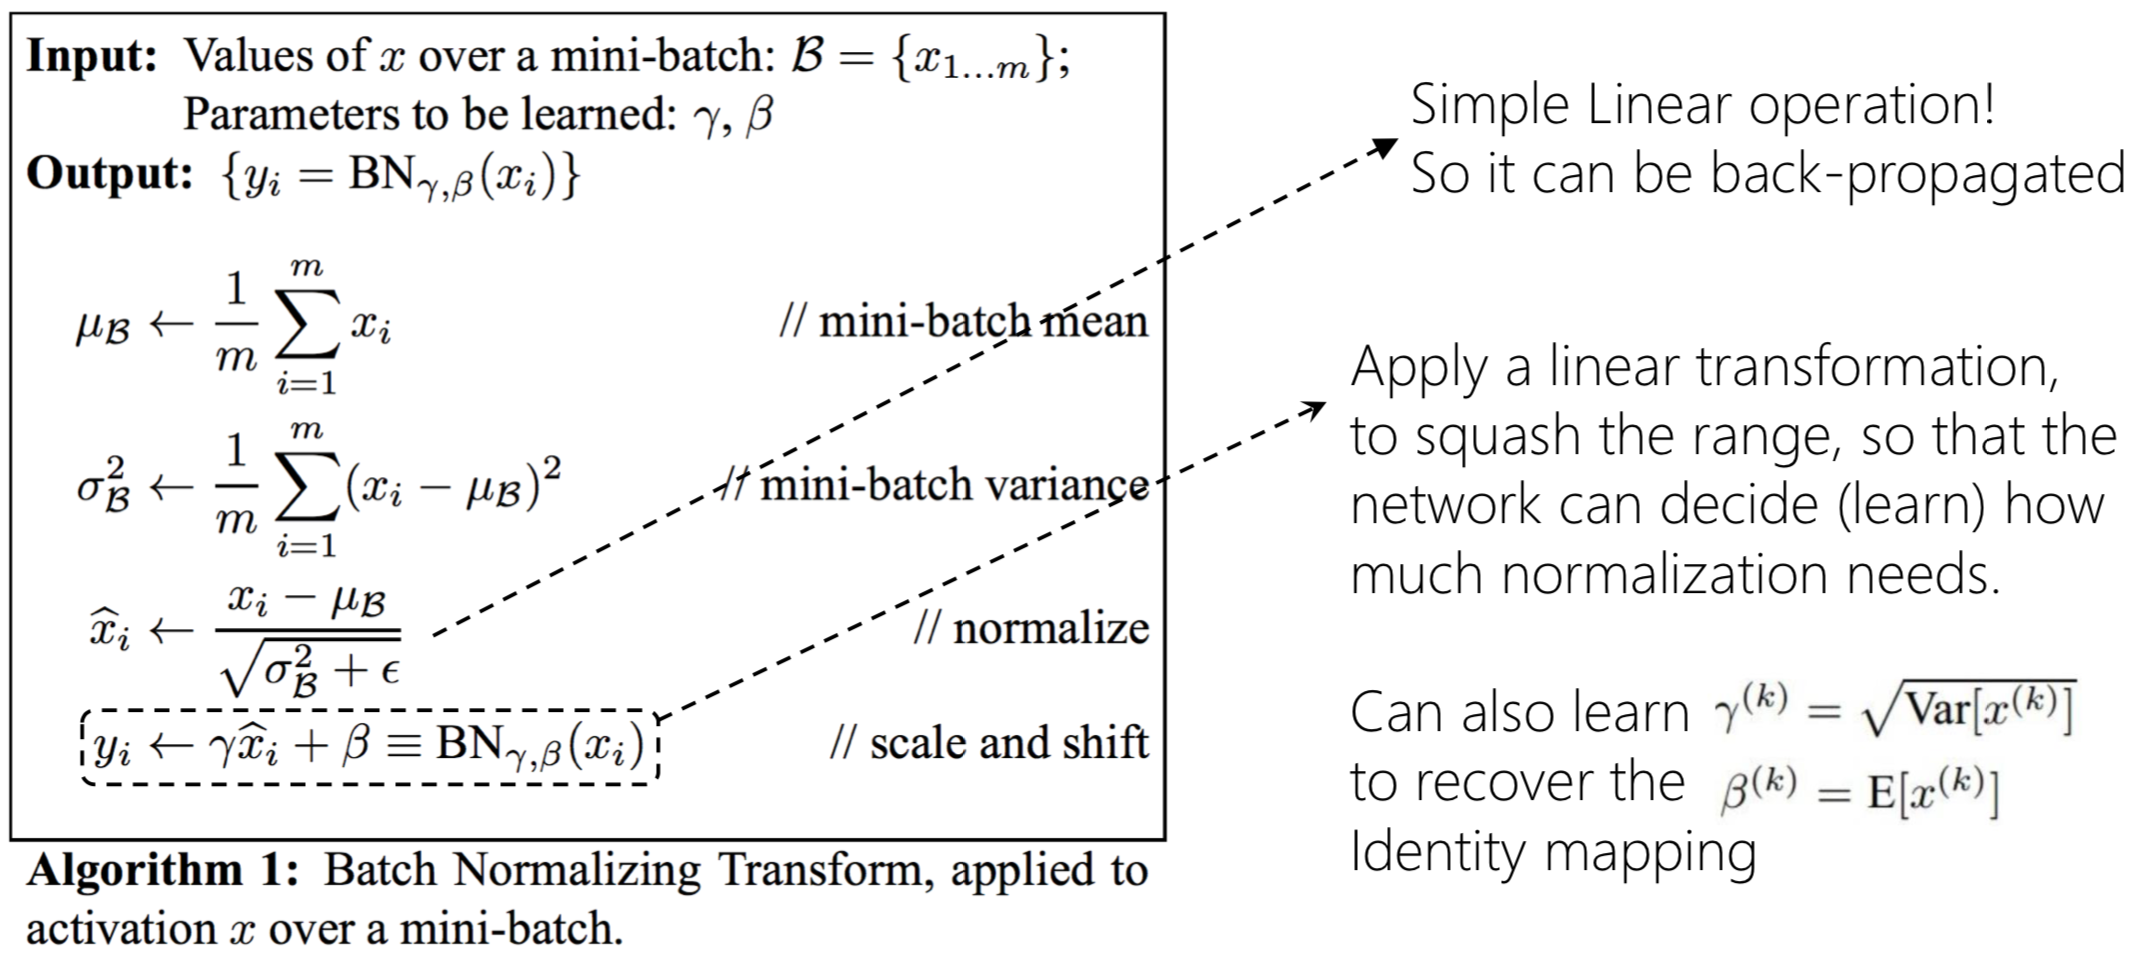
\includegraphics[width=14cm, height=6cm]{images/batch_norm.png}
        %\captionof{figure}{The model pipeline.}
        %\label{fig:flow_fig}
\end{minipage}
\vspace{0.2cm}


%It is a specific layer network. In practice, usually what you do is to normalize zero mean and unitary-variance of the input because it's known to be better in terms of 'covariance shift': if you have only shift in covariance, or in mean between the test and the training, if you normalize (they would be the same? reg.7 1:04:43). So the idea is that you take the original data and you normalize centering the data with zero mean and unitary variance for each of the feature, so you are sure that your data are in a square of size one. This is something that you can do for the input too. This may be useful in each level of representation.

%Another relevant thing is that want you would like to do with your data is to have the same distribution; in mini-batch training, you would like that all the batches have the same mean and the same variance. So the idea is to add as part of the training,  normalization procedure: you would like to normalize the data as they pass through the layer of the networks. This means that you want to force all the activation to take value as unitary-variance at the beginning of the training and during the training. To do this you can use what it is called Batch Normalization: it is something that can be put between the weighted sum of the input and non-linearity. Putting it in the middle, you have a normalization while you perform training. You can do back-propagation even if in the middle there is Batch Normalization layer since normalization (which is removing the constant value and dividing by the constant value) is differentiable. It is relevant because you can learn, or adapt, the number to substitute for the mean and the variance.

As you have noticed, during:
$
\widehat{x}_{i} \leftarrow \frac{x_{i}-\mu_{B}}{\sqrt{\sigma_{B}^{2}+\epsilon}}
$
we add some random noise to avoid division by zero.

In practice: 
\begin{enumerate}
    \item Each unit’s pre-activation is normalized (mean subtraction, stddev division)
    \item During training, mean and stddev is computed for each minibatch
    \item Backpropagation takes into account the normalization
    \item At test time, the global mean/stddev is used (global statistics are estimated using running averages during the training)
\end{enumerate}{}

It has shown to:
\begin{itemize}
    \item[--] Improve gradient flow through the network
    \item[--] Allows higher learning rates
    \item[--] Reduces the strong dependence on initialization
    \item[--] Acts as a form of regularization slightly reduces the need for dropout
\end{itemize}{}

%slide 33
%So what happens in batch normalization is more or less the following: each unit's pre-activation is normalized, it means you remove the mean and divide by the standard deviation. Then during the training you learn which is the mean and the standard deviation. At each mini-batch, you compute the mean and the standard deviation of the mini-batch. The mean is the mini-btach sum of the input, the mini-batch variance is (guardare pag 32). You update the data using these two numbers. You can also rescale and shift the output.  Qui

%$$
%\widehat{x}_{i} \leftarrow %\frac{x_{i}-\mu_{B}}{\sqrt{\sigma_{B}^{2}+\epsilon}}
%$$
%to avoid division by zero we add some random noise. So it is a huge differentiable mathematical formula, so you can derive the error wrt to this and you can learn the scale and the beta parameter used for this dataset and you should adapt through multiple mini-batch: at test time you have the global mean and the global standard deviation of the whole train. Basically this layer is normalizing the data within the batch having zero mean and unitary variance. 
% Neural Networks and Template Matching, Facing Overfitting, Training tricks and Vanishing gradient, sono dentro Training and Overfitting?
\section{Convolutional Neural Networks}
Convolutional neural networks are the tools for performing most of the visual tasks, like classification and detection, and they are probably the most widely known deep learning model. 
%(sta facendo un recap tipo? manca una lezione forse?)

\subsection{The Feature Extraction Perspective}
Instead of just feeding directly our image to a classifier, we perform some preliminary step to extract features from the images, we will perform some preliminary algorithm that maps our image into a vector which is informative for defining the label where the image belongs to. You are not trying to directly handle the image has a vector but you extract some meaningful information out of the image in order to feed this additional information to a standard classifier. Feature extraction is a winning strategy, for example it lets you embed some a-priori additional information you have on your data. One way is to do exploratory data -analysis and to draw some rule from what comes out, identifying the various classes by some rule based feature; the problem with this kind of features is that is difficult to design complex relations which involve many variables in which sometimes it's not easy to separate the variables. Neural networks and things like SVM on the other side are able to learn more complex relationships among variables that include many variables. An option is to add hand written features that come from our expertise to the neural network. For natural images, the hand crafted approach doesn't work and you have to go to the data driven approach. This means using Convolutional Neural Networks. Before using CNN, we need to understand how convolution works.

\subsection{Convolution}
Convolution it's, up to some change of sign, exactly as \textit{correlation}. Convolution is a linear transformation applied to an image.
\begin{center}
    $T[I](r, c)=\sum_{(x, y) \in U} w(x, y) * I(r-x, c-y)$
\end{center}
If you have an image and a filter (which is nothing more but a small image); we can consider the weights as a filter $H$ and the filter entirely defines the convolution, which operates the same in each pixel:
\begin{center}
    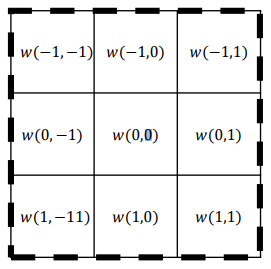
\includegraphics[width=0.3\textwidth]{images_CNN/filter.PNG}\par\vspace{1cm}
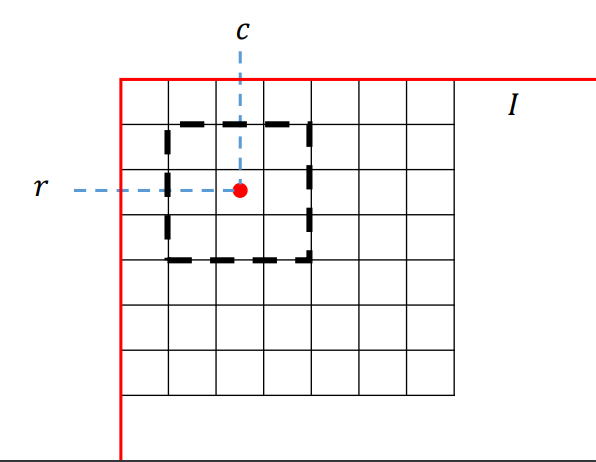
\includegraphics[width=0.45\textwidth]{images_CNN/imag.PNG}\par\vspace{1cm}
\end{center}

The convolution of the input image against this filter is still an image. The size of the output image in principal should be the same of the input one. The same operation is performed in each pixel of the input image and we get a value for each pixel, which is gonna be just the linear combination of the pixel values in a neighbor of the pixel (which has the same size of the pixel).\\
So you take your filter, you place it over the image right in the position where you want to compute the output (in this case you place the filter so that the center goes in $(r,c)$) and the output is the linear combination of the pixel values using these coefficients as weights for the linear combination. \\
Convolution is the process of adding each element of the image to its local neighbors, weighted by the kernel. What happens on boundaries?\\
There are different options; the simplest thing is to use 0 padding, so you set 0s where the filter goes out of the image (so its black), otherwise you can compute the output of the convolution only at those pixels where the filter can be entirely included in the image. Note that a minus sign means that you have to flip your image, it's exactly the same if you flip your filter, it's important only if you define the filters but in general we will learn the $w$. Convolution was already used in signal processing, it's used to compute the Fourier transformed, it wasn't invented for neural networks. \\
Correlation is the same but in correlation you have the plus sign whether in convolution you have the minus sign. 
%(inizia a fare esempi a caso)

\subsection{CNN Layers}
CNN are networks that take as input an image and provide as output as any neural networks, for example for classification, a set of probabilities associated to each class. For example, for the CIFAR dataset we take as input 32x32x3 images and we provide as output 10 values which are the posterior probabilities over the 10 classes. In a CNN you see some structure of the image which is preserved, you see the feature maps. As you move deeper you see 
%(guarda slide) 
that they are increasing in number an decreasing in size, each of this images are layers of the volume; feature maps become smaller but deeper so the height and width of the volume decrease whether the dimension increases. In order to perform this operation that reduces the size and increases the dimension, you use 3 different layers: 

\begin{itemize}
    \item convolutional layers
    \item activation functions
    \item pooling layers, in particular max pooling
\end{itemize}

\subsubsection{Convolutional Layers}
In a CNN you have a set of filters given for each layer and these filters represent the network parameters. Let's see what is the output of the convolution of this image against a filter which is, for example, 3x3x3:

\begin{center}
    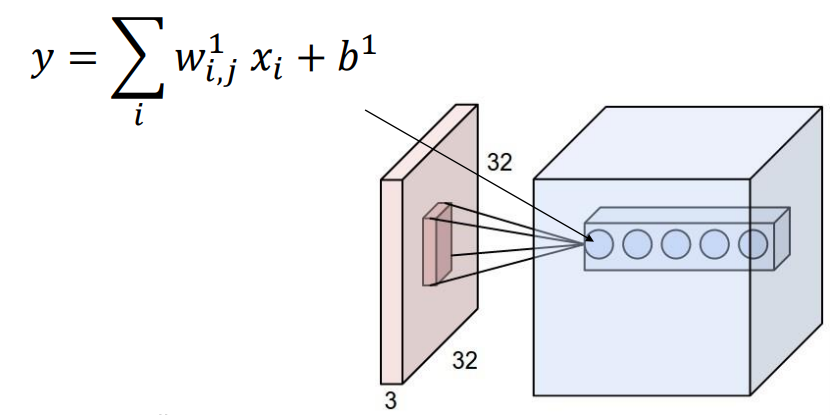
\includegraphics[width=0.5\textwidth]{images_CNN/clayers.PNG}\par
\end{center}
Remember that each filter has to have the same depth as the input volume, in this case you have 3 channels so the filter will be 3x3x3. Each pixel in the output image is gonna be given by the filter and the pixel values of your image in a neighbor of the same pixel, as we saw before. What we have in that point 
%in the image 
are the weights $w$ multiplied by the input $x_{i}$ plus some bias, it's a linear combination. You compute different filters and the output images becomes deeper. Increasing the depth is done simply by adding multiple filters; the parameters of a convolutional layer are all the weights that are stored in filters plus one bias associated to each filter.

%As you can see in the next slides,
As you can imagine, one input image with one filter gives one output map, two filters give two output maps etc. The important thing is that the filter has to have the same depth as the input map, and the filter is applied to the whole spatial extent of the input, and adding more filters increases the number of output maps.

If you feed a network with 3 input maps, what happens is that all your filter will be 3 different layers and the filters corresponding to the moving output map are those that are also moving. How many parameters does this layer have?
\begin{center}
    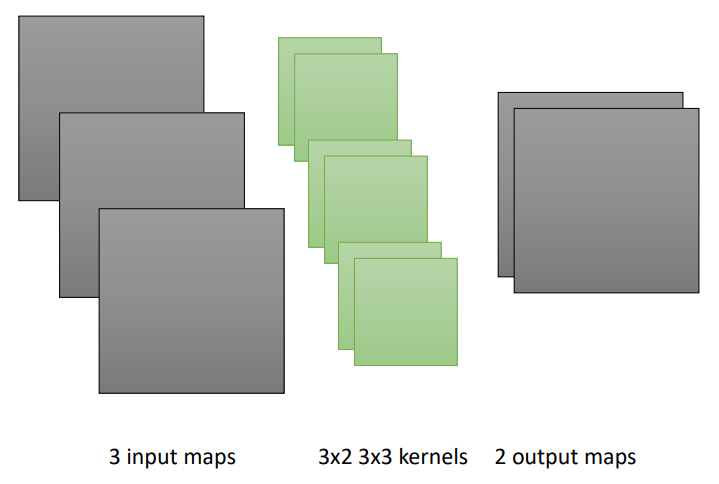
\includegraphics[width=0.5\textwidth]{images_CNN/layers.PNG}\par
\end{center}
Each layer has 9 parameters (3x3), but each filter has 3 layers so its 9x3=27 for each filter, x2=54; moreover you have to consider the bias, one for each filters. So: 54 for the filters + 2 biases = 56 trainable parameters. What's really important is that convolution mixes all the input channels. Typically you have small filters in these networks, they have a negligible size w.r.t. the image size.

\subsubsection{Activation Functions}
Convolutional layers perform linear combinations, so what you get at the end is again a linear combination. Like in the multilayer perceptron, you have to introduce some non-linearity and you do this with the activation function, otherwise the CNN would be equal to a linear classifier. The most popular is the Rectified Linear Unit (RELU):
\begin{center}
    $T(x)=\left\{\begin{array}{ll}{x,} & {\text { if } x \geq 0} \\ {0,} & {\text { if } x<0}\end{array}\right.$
\end{center}
Another option is a variant of the RELU called leaky RELU:
\begin{center}
    $T(x)=\left\{\begin{array}{ll}{x,} & {\text { if } x \geq 0} \\ {0.01 * x} & {\text { if } x<0}\end{array}\right.$
\end{center}
These functions activates the neurons performing some thresholding on the feature maps. Other options are:


\subsubsection{Pooling Layers}
These layers reduce the spatial extent of the input volume. The most popular is the MaxPooling layer which operates independently on each slice. 
\begin{center}
    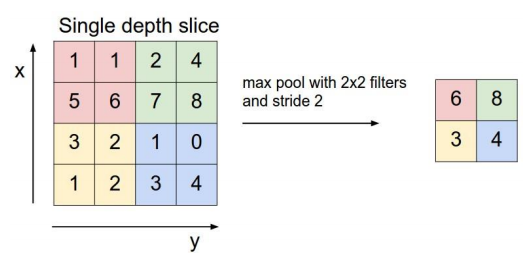
\includegraphics[width=0.5\textwidth]{images_CNN/maxpool.PNG}\par
\end{center}

\subsubsection{Fully Connected Layer}
When you get to the end reducing the spatial extend with the pooling layers, what you get is that your volume will have a special extent equal to 1, so it's just a large vector. This vector is the feature vector and with it you train a multilayer perceptron, which is called a fully connected layer.

\vspace{1cm}

The first CNN goes back to 1998, the LeNet-5. After that NN were forgotten for a while until a CNN model won the ImageNet competition of 2012, AlexNet, which was the first deep CNN. There are two main reasons for which they had difficulties in spreading after 1998: heavy computation and lack of data. Moving to these days, a lot of things have changed: on one side new mosfet technologies, fast CPU, graphic computation, on the other side amazingly increasing data of all kinds are created each second. These two factors, parallel fast computing and a lot of training data, really played a crucial role for the escalation of neural networks.
% Training with data scarcity ?
\section{Image Segmentation}
The goal of Semantic Segmentation is: \\
Given an image $I$, associate to each pixel $(r,c)$ a label from $\Lambda$. \\
The result of segmentation is a map of labels containing in each pixel the estimated class.\\

Remark: segmentation does not separate different instances belonging to the same class. That would be instance segmentation. \\ \\
The training set is made of pairs $(I,GT)$, where the GT is a pixel-wise annotated imgae over the categories in $\Lambda$.

\subsection{Fully-Convolutional Networks}
CNNs are meant to process input of a fixed size. The \textit{convolutional} and \textit{subsampling} layers operate in a sliding manner over image having arbitrary size. The \textit{fully-connected} layer constrains the input to a fixed size. \\

\begin{wrapfigure}{r}{8cm}
    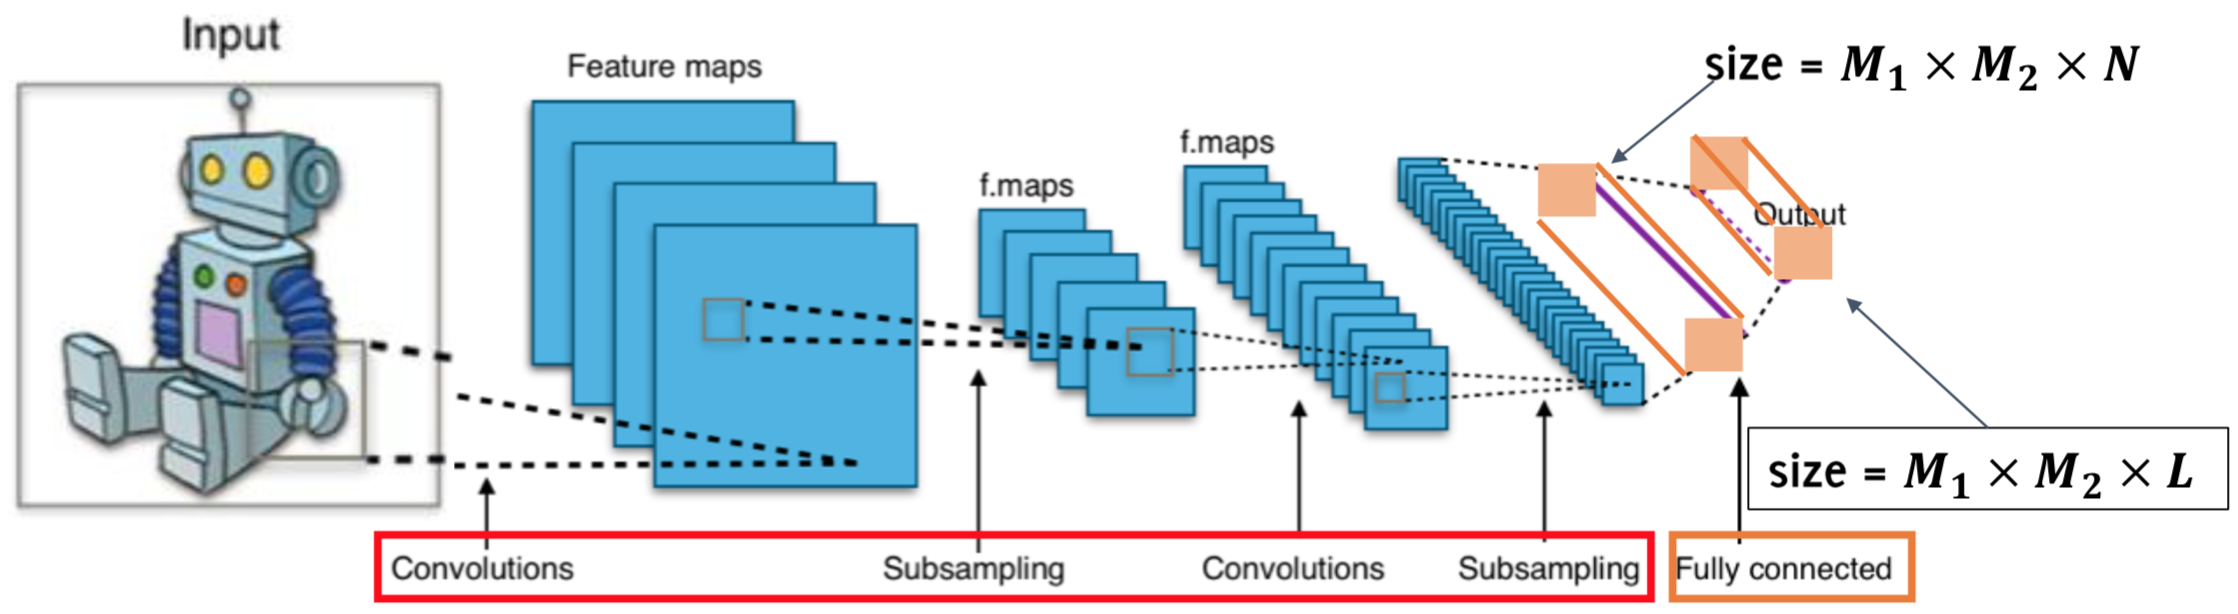
\includegraphics[width=7.5cm, height=3cm]{images/cnn_segm.png}
    %\label{fig:lstm_org}
\end{wrapfigure}  

If I fed the network with larger images, convolutional filters can be applied to volumes of any size, yielding larger volumes in the network until the FC layer. What breaks is in the FC layer because instead of having $1*1*N$, it processes a volume of size $M_1 * M_2 * N$. Thus, CNN cannot compute class scores, yet can extract features!

\begin{wrapfigure}{l}{9cm}
    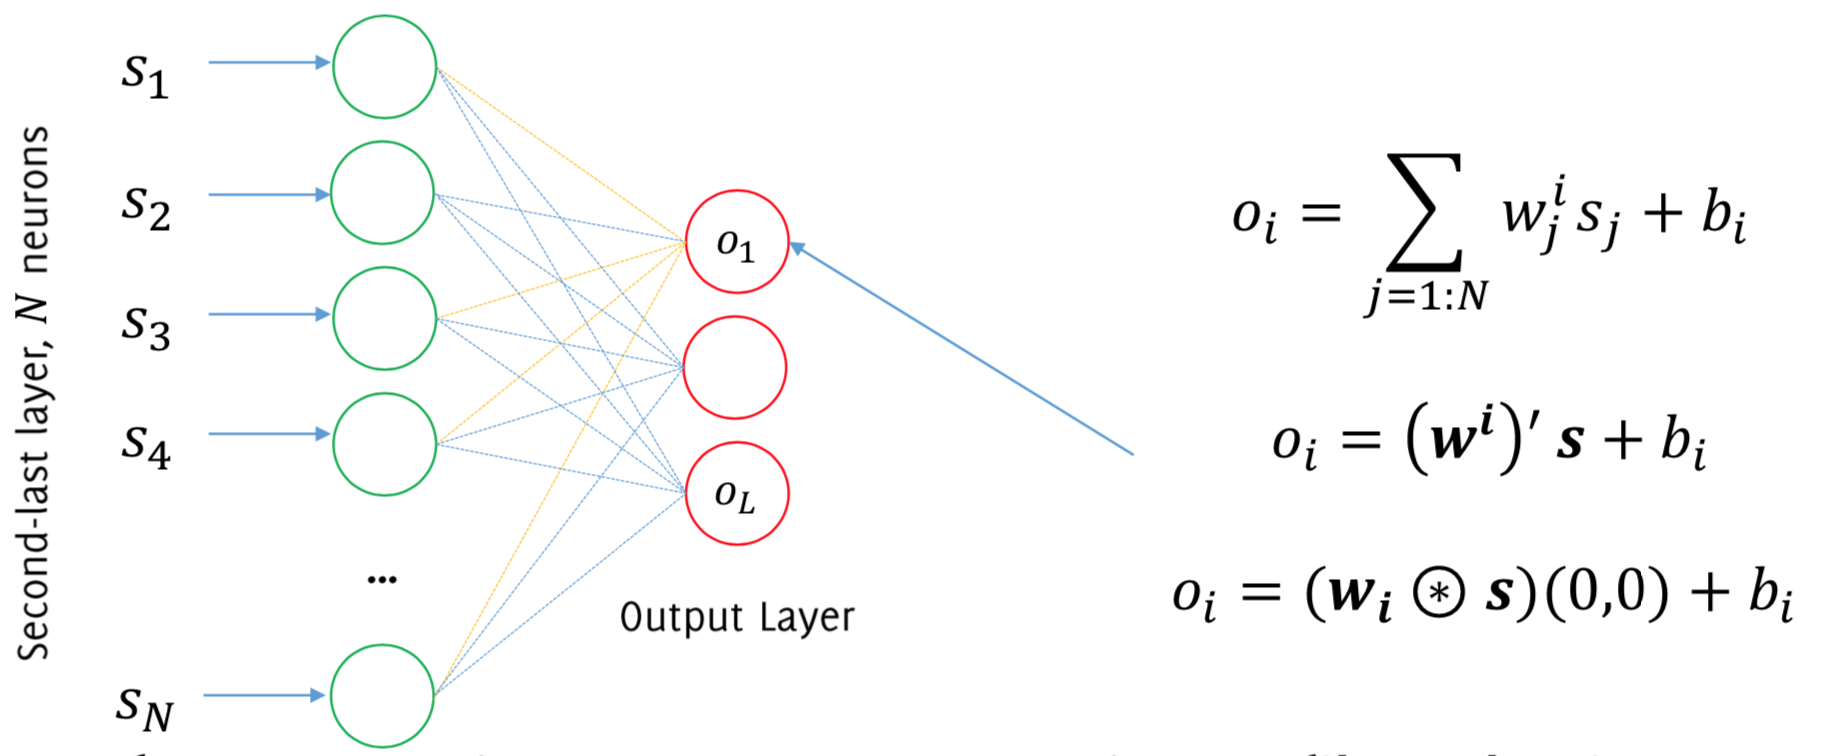
\includegraphics[width=9cm, height=3.5cm]{images/fc_to_cnn.png}
    %\label{fig:lstm_org}
\end{wrapfigure}  

However, since the \textbf{FC} is \textbf{linear}, it can be represented as convolution! Weights associated to output neuron i: $$\boldsymbol{w_i} = \left\{w_{i,j}\right\}_{i=j:N}$$ \\ \\ \\
A FC layer of $L$ outputs is a 2DConv Layer against L filters having size $1*1*N$. Each of these convolutional filters contains the weights of the FC for the corresponding output neuron. This transformation can be applied to each hidden layer of a FC network placed at the CNN top.  \\ 
For each output class we obtain an image, having: 
\begin{itemize}
    \item Lower resolution than the input image
    \item Class probabilities for the receptive field of each pixel
\end{itemize}{}

%reg.11 inizia da slide 5
%The output of segmentation can not separate between different instances (that is Instance Segmentation). 
%When we transform our model from a classification network to a Fully-Convolutional network, we can get a few heatmaps which contain for each pixel a sort of output of the scores. 
%In a cnn the first part is the entire convolutional part, then there is the fully connected one. If I change the input size of the image, the network is trained with the images of that size. If I fed the network with larger images, what breaks is in the fully connected part because instead of having a size of $1x1xN$, we obtain a size of $M_1 x M_2 x N$. You can modify a fully-connected layer which takes N input to provide L output, you can transform this (credo the fully-connected part) as a convolutional layer with convolution (qualcosa reg.12 00:44) size 1x1, and the filter has the size 1x1xN. 

%This filter has just re-writing the weights of the first output neuron.
So how many filter should I use to replace the fully-connected layer into a convolutional layer? \\
L filters: one filter per each output neuron and each filter has size $1*1*N$. We can move each fully-connected layer that takes $N$ input and provides $L$ output as a convolutional layer having $L$ filter each one having size $1*1*N$. This transformation can be applied if you have a multi-layer perceptron too.
%What the 1x1 convolution does is to mix all the filters together, all the layer together without performing any special mixing and providing this mixing as output. 
What you get is, given an image, you have multiple small images (\textit{heatmaps}), one for each classes, and these small image contains a score which tell you how much likely there is something that looks like something, for instance a wheel. 
\subsubsection{Simple Solutions}
The first way to perform segmetation is: take the heatmaps, for each pixel take the most likely class. So given an input image to fed a fully-convolutional network, you get the heatmaps: with these multiple heatmaps, for each pixel we take the argmax among those heatmaps for that pixel, which corresponds to the most probable class. However that would be a very \textbf{coarse estimate} \\

\begin{minipage}{\linewidth}
        \centering
        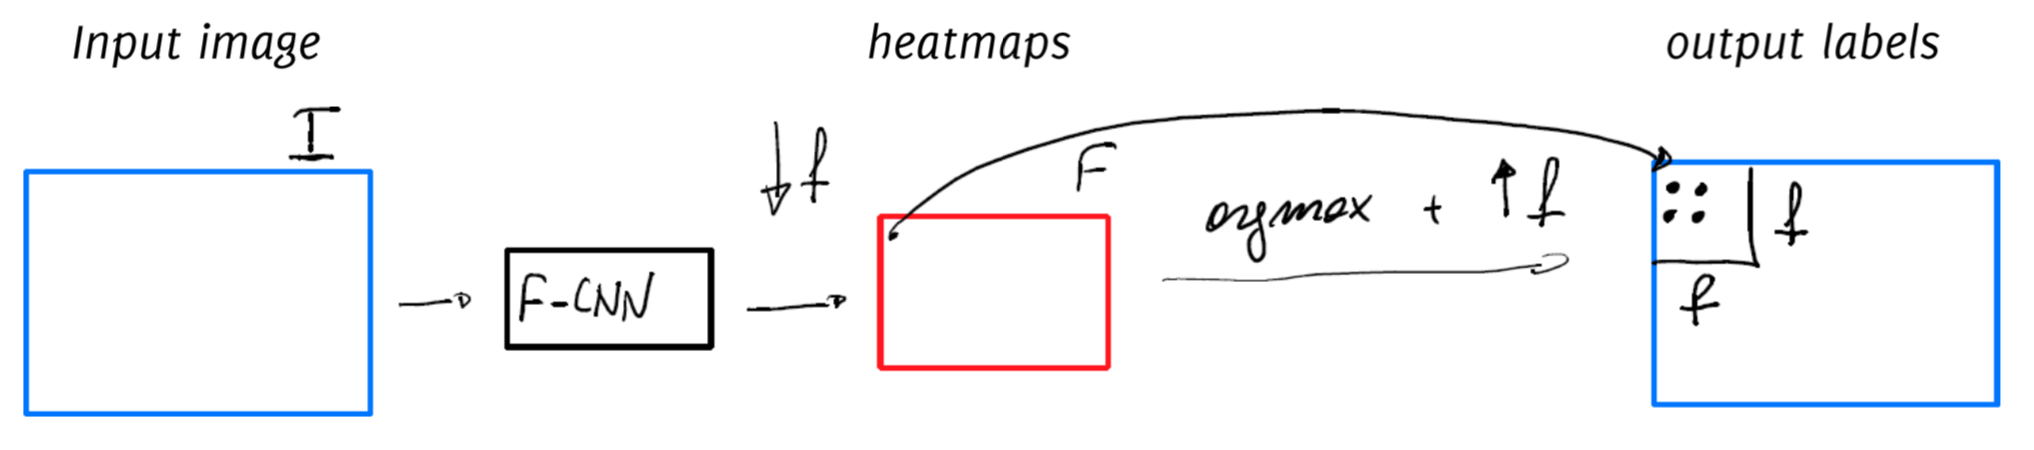
\includegraphics[width=8.1cm, height=3cm]{images/simple_solution_segm.png}
        %\captionof{figure}{The model pipeline.}
        %\label{fig:flow_fig}
\end{minipage} \\


Another option would be the \textit{Shift and Stitch}: \\
\begin{wrapfigure}{l}{9cm}
    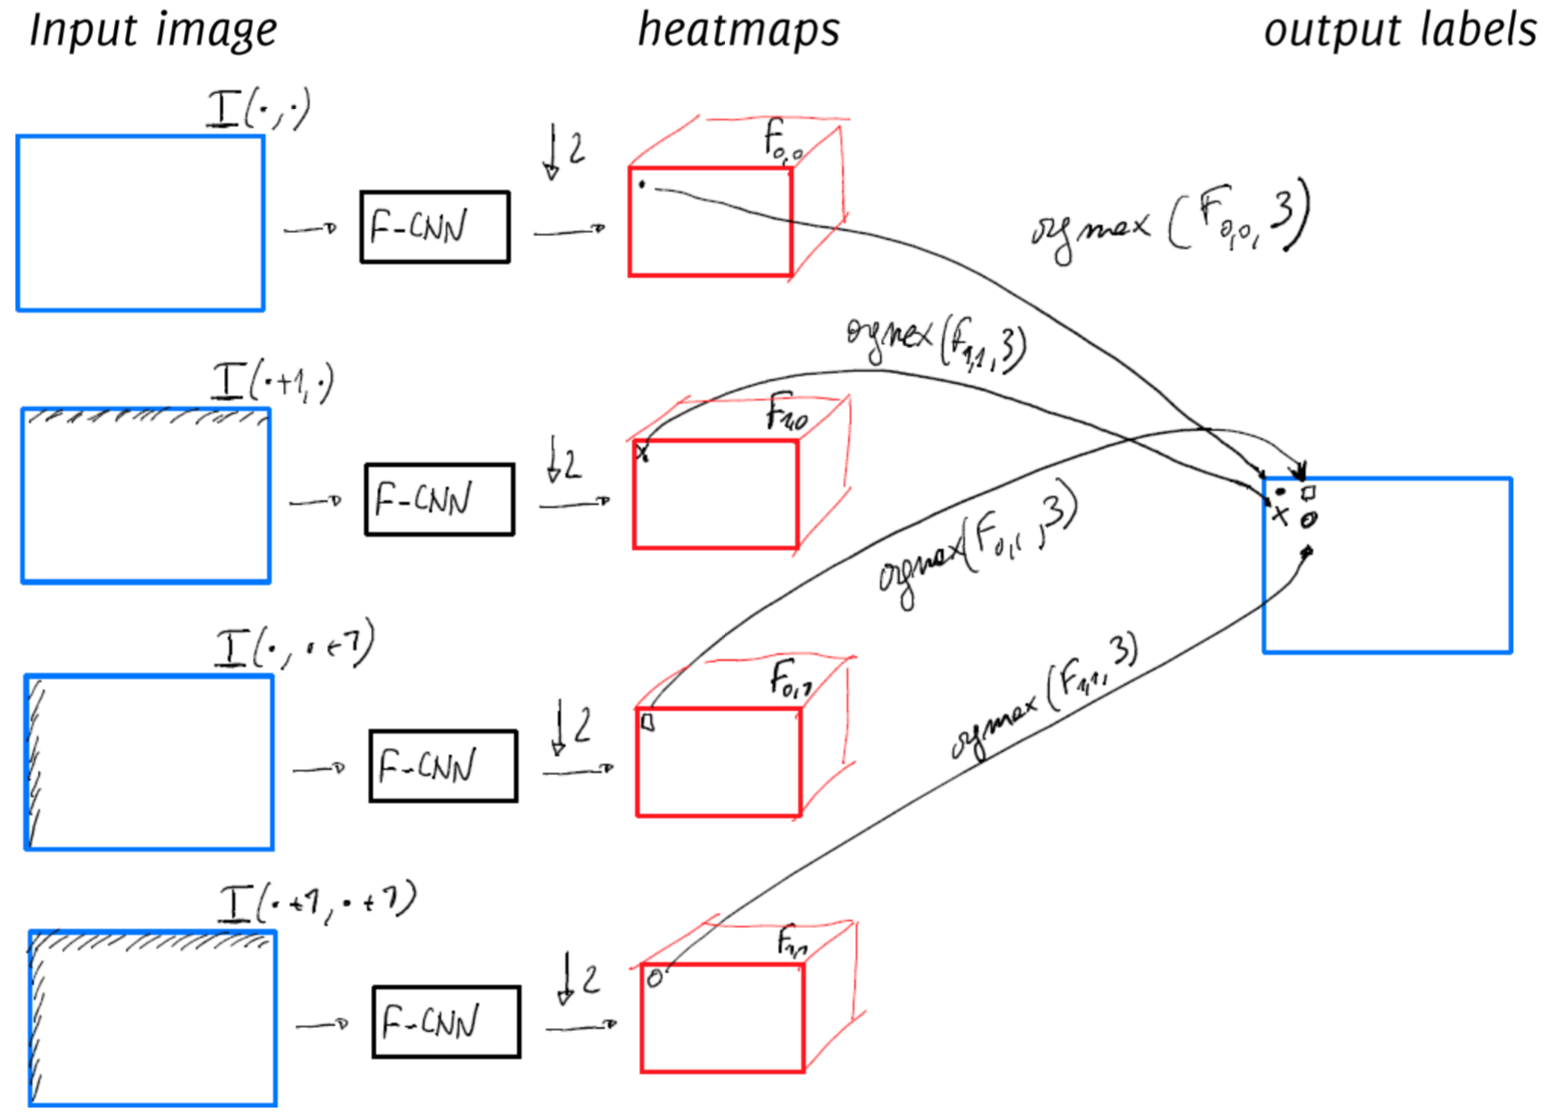
\includegraphics[width=9cm, height=8cm]{images/shift_stitch.png}
    %\label{fig:lstm_org}
\end{wrapfigure}  
Assume there is a ration $f$ between the size of the input and of the output heatmap. You have to:
\begin{itemize}
    \item Compute the heatmaps for all $f^2$ possible \textit{shifts} of the input $\left( 0\leq r, c < f \right)$
    \item Map predictions from the $f^2$ heatmaps to the image: each pixel in the heatmap provides prediction of the central pixel of the receptive field
    \item Interleave the heatmaps to form an image as large as the input
\end{itemize}{}

This exploit the whole depth of the network, however the upsampling method is very rigid. \\


%for each input image, I shift my images of 1 pixel left, 1 pixel down and so on. For each input image I make it like 4 times, with shift and without, obtaining 4 different blocks. Then there is the stich operation, given the outputs, instead of feeding only the input image, you feed also the image shifted down, the image shifted left, and the image shifted down-left. You perform the argmax and now (qualcosa incomprensibile). The major drawback of the shift and Stich operation is that is this sort of upsampling which means (this, there, there to that non si capisce una sega). \\

\begin{wrapfigure}{r}{7cm}
    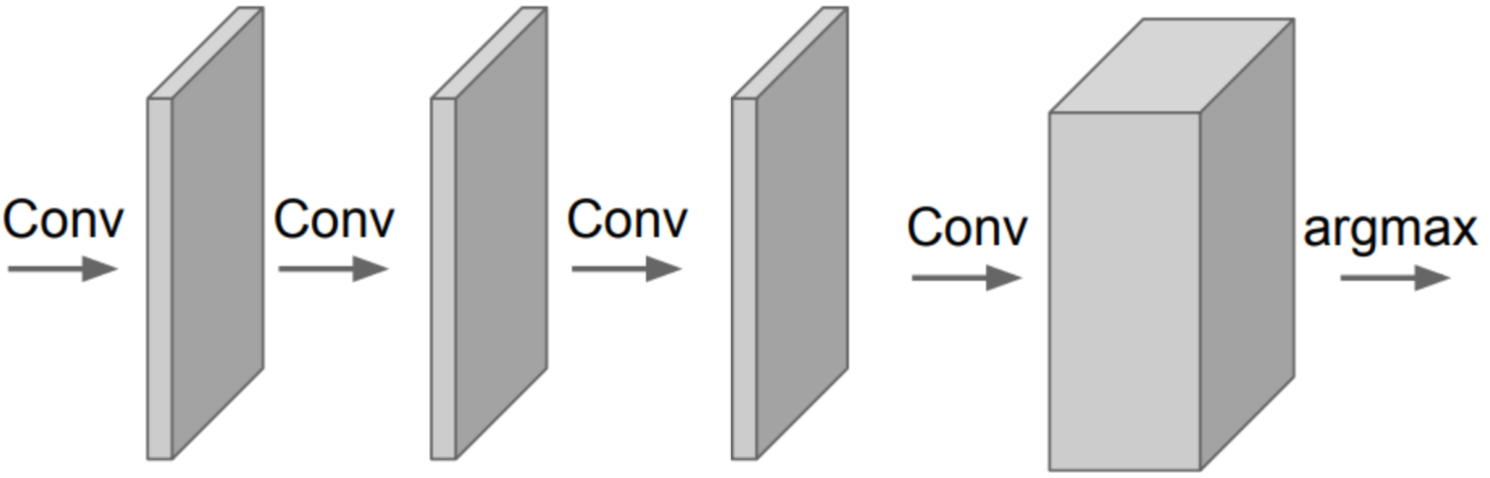
\includegraphics[width=7cm, height=3cm]{images/only_convolutions.png}
    %\label{fig:lstm_org}
\end{wrapfigure}  

The last possible approach is to perform \textit{Only Convolutions}: you can design a network without any downsampling, without any pooling. In principle, you can get in output an image with the same size, but the major drawback is that you do not increase enough the receptive field for having meaningful information $\Rightarrow$ Very inefficient. \\

\subsubsection{Main Solution}
On the one hand we need to "go deep" to extract high level information on the image. On the other hand we want to stay local not to loose spatial resolution in the predictions.\\
Semantic segmentation faces an inherent tension between semantics and location: 
\begin{itemize}
    \item global information resolves what, while
    \item local information resolves where
\end{itemize}{}
Combining fine layers and coarse layers lets the model make local predictions that respect global structure. \\
An architecture like the following would probably be more suitable for semantic segmentation: \\

\begin{minipage}{\linewidth}
        \centering
        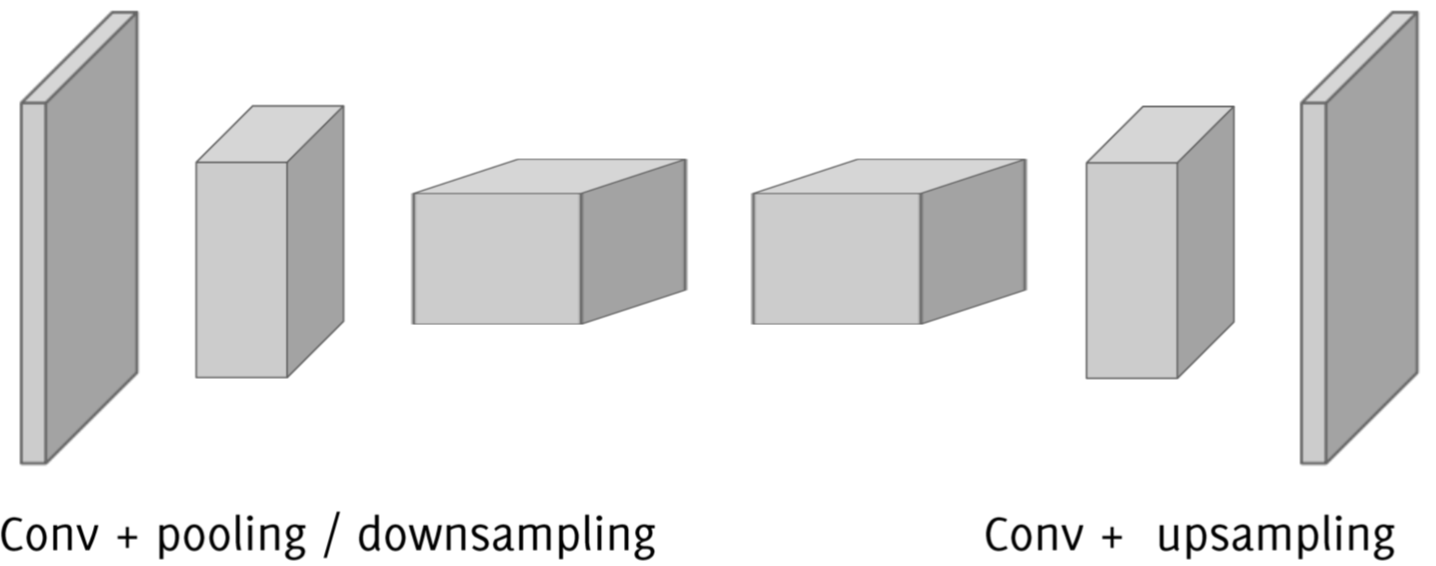
\includegraphics[width=8.1cm, height=3cm]{images/segm_architecture.png}
        %\captionof{figure}{The model pipeline.}
        %\label{fig:flow_fig}
\end{minipage} \\

In the first part you go deep encoding semantic information; in the second part, perform upsampling and get high resolution output to recover local information: this part is meant to upsample the predictions to cover each pixel in the image. Increasing the image size is necessary to obtain sharp contours and spatially detailed class predictions. 
%Another option is, if you have some problem, you can design a network without any downsampling, without any max pooling. You can get in principle in the output an image with the same size, but you do not increase enough your recepting field for having meaningful information in the final layer.
%What we want to have during segmentation is:
%'semantic segmentation faces an inherent tension between semantics and location', so in order to understand the content of the image you need to go deep, you need to have this squeezing of your volume to have some information that refers to multiple pixels. In the other have, to have accurate predictions and accurate estimate, you need to avoid this operation of squeezing and keeping the highest resolution as possible. The idea of the original paper is to combine fine layers and coarse layers to let the model make predictions over a global structure. 
%So what is said in the paper is firstly to go deep and then doing the opposite operation, so increase the spatial resolution in order to have the same input resolution. What you want is that the second half of the networks can increase the spatial resolution preserving the semantic information. 

%So we have some convolution and some upsampling. Reducing the size of these squares, you increase the size of the pixels. 
\subsection{Upsampling}
Linear upsampling of a factor $f$ can be implemented as a convolution against a filter with a fractional stride $1/f$. \\
Upsampling filters can thus be learned during network training. \\
Upsampling can be performed in several ways: 
\begin{itemize}
    \item Nearest-Neighbor: the output is of a larger size and the pixel value correspond to the value of the nearest pixel.
    \item Bed of Nails: the output pixels correspond to the input ones, located in the top left corner of the output sub-squares, and the remaining pixels are filled with zeros.
    \item \textbf{Max Unpooling}: you have to keep track of the locations of the max during max-pooling. Remember which element was the max and, during max unpooling phase, use those positions to upsample the input and locate the max valued pixel in the same position as original.
\end{itemize}{}

\begin{minipage}{\linewidth}
        \centering
        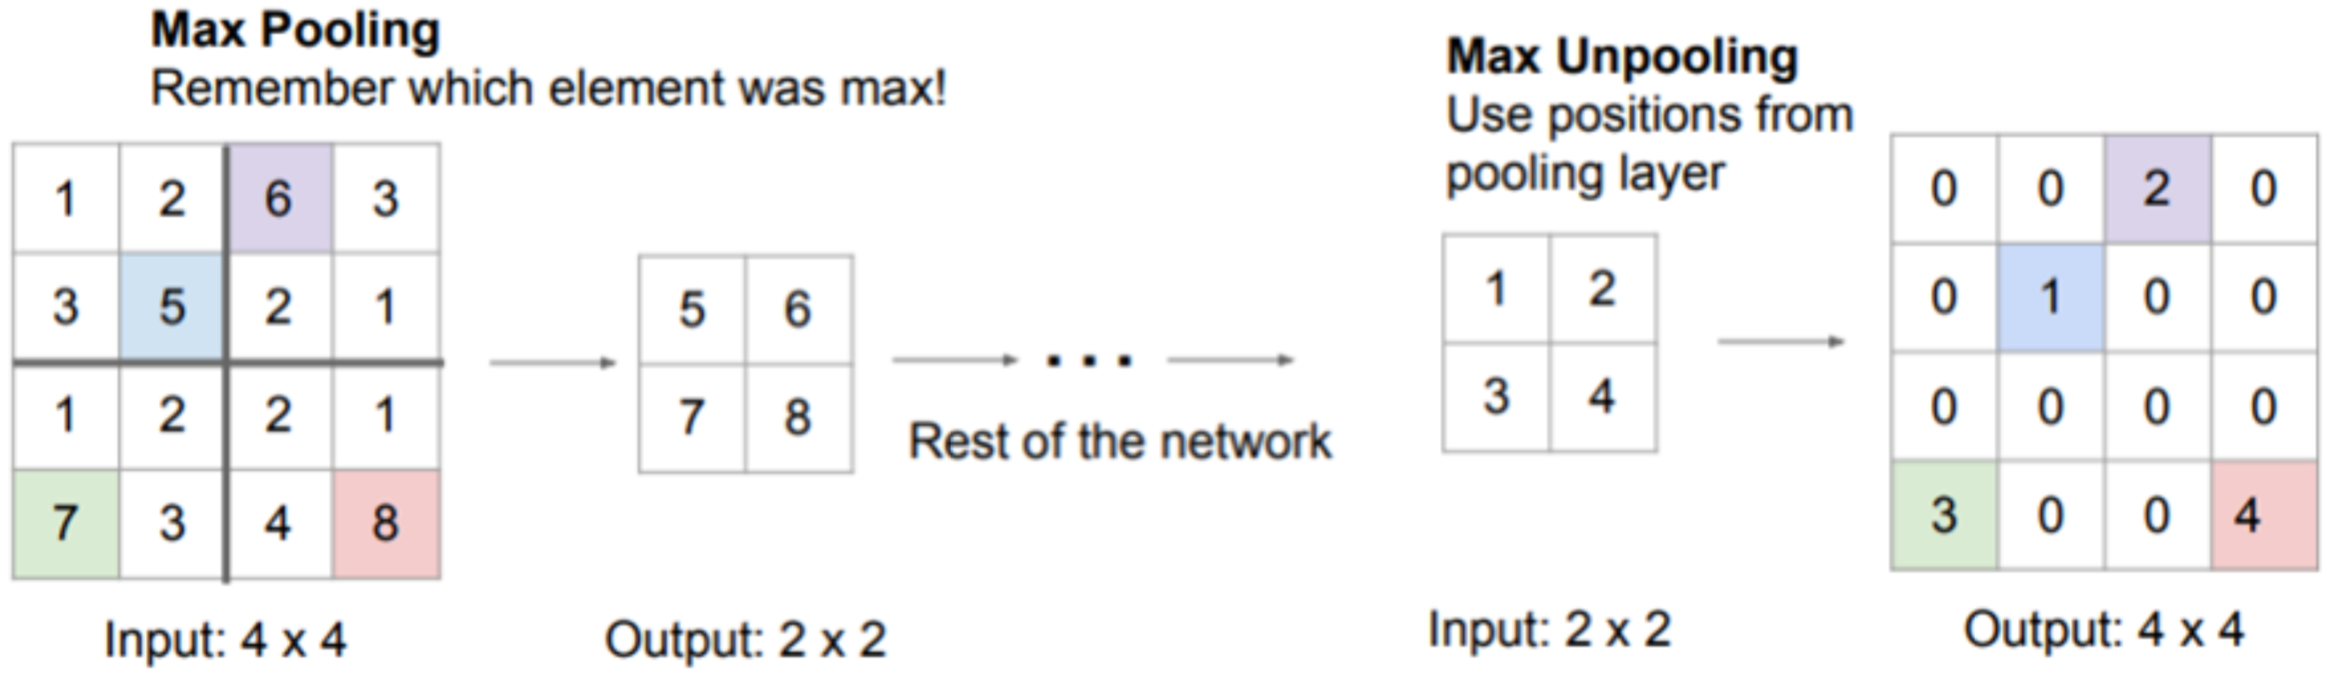
\includegraphics[width=15cm, height=5cm]{images/max_pooling.png}
        %\captionof{figure}{Logical Architecture}
        \label{fig:log_arch}
\end{minipage} \\

How to perform upsampling?\\
\textbf{Transpose Convolution} can be seen as a traditional convolution after having upsampled the input image. In this way our network can learn how to upsample optimally. \\
A classical convolution operation forms a many-to-one relationship: in general, the convolution operation calculates the sum of the element-wise multiplication between the input matrix and the kernel matrix; from a matrix you get only one value.  \\ \\
The idea of Transpose Convolution is to going backward, it's a one-to-many relationship: we want to associate one value to a matrix of values. If your input is a $2*2$ matrix, you want a $4*4$ output and you have a filter of size $3*3$ [stride 2, pad 1], get the first pixel value of the input and multiply it by the kernel values: this operation returns a filter that has been rescaled by the value of the image, so the input gives weight for the $3*3$ filter. Compute the same operation for the other pixels and sum the values where output overlaps. \\

\begin{minipage}{\linewidth}
        \centering
        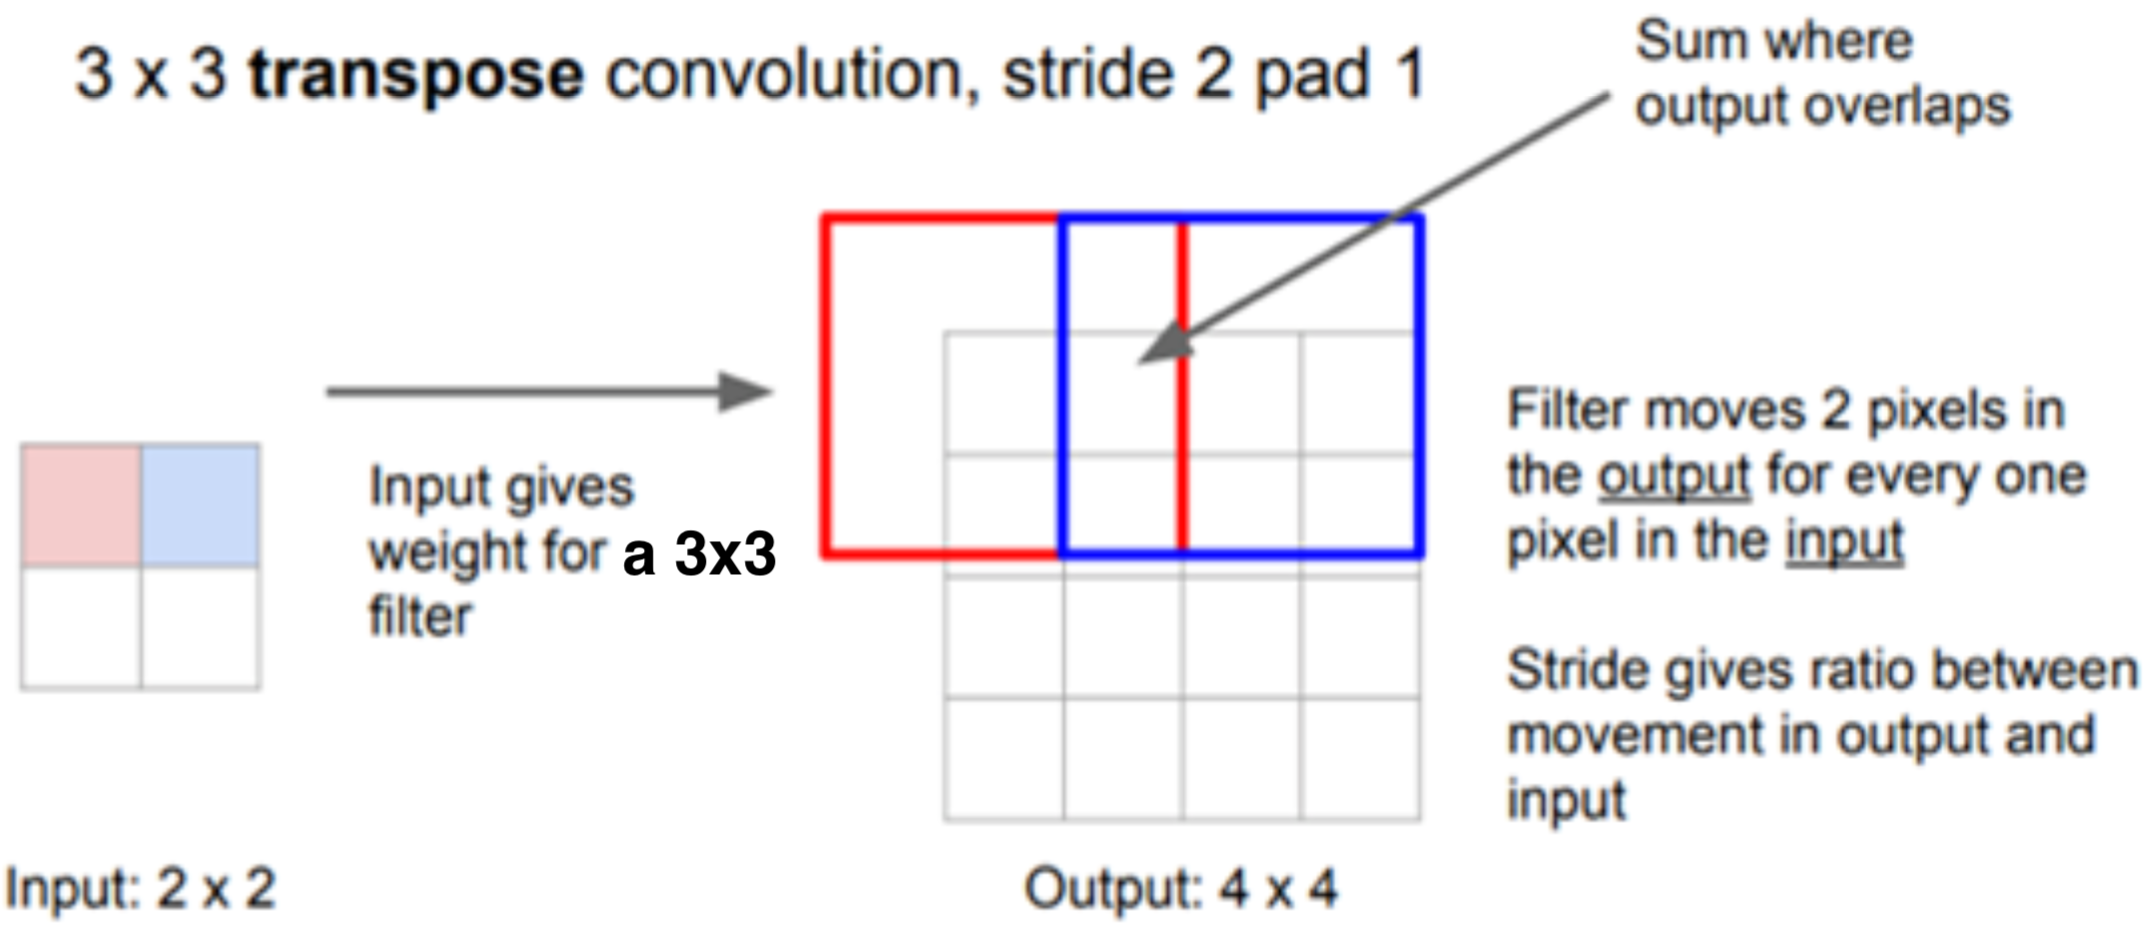
\includegraphics[width=15cm, height=5cm]{images/transpose_conv.png}
        %\captionof{figure}{Logical Architecture}
        \label{fig:log_arch}
\end{minipage} \\ 

%There are standard upsampling option like nearest-neighbours: the output is of a larger size and the pixel value correspond to the value of the nearest pixel. There is max-unpooling: when you perform the max pooling, you keep track of the location where the maximum was. So if there is the input in the contractive part of the network [so 5,6,7,8 nell'immagine] and instead of keeping the max values and propagate to the network, you keep track of the location inside the activation maps where these pixels were. So when you get back to the same point in the network to the corresponding layer you put the max values in the original location where they were. In this way you double the image size. 
%The idea of how to perform this parametric upsampling, it through the \textbf{Transpose Convolution}: change the role of the filter of the image; the input is 2x2 and you want a 4x4 output and you have a filter 3x3. So the transpose convolution is like, you take the value of the 2x2 image and you multiply it by you 3x3 filter and this gives you as output a filter that has been rescale by the value of the image. Then you place these values and you actually obtain 9 estimate, each one equal to the value of the filter rescale by the value of the image. Then you move by one pixel (depend on the filter definition) and you take this value of the image and you multiply by the same filter and you get 9 estimation. Then you sub the values on those location where the outputs overlaps. 
These predictions however are very coarse. Upsampling filters are learned with initialization equal to the bilinear interpolation. The solution is to introduce \textbf{Skip Connections}.

\subsection{Skip Connections}
There was some information that was captured in the initial layers and was required for reconstruction during the up-sampling. If we would not have used the skip architecture that information would have been lost. So the information that we had in the primary layers can be fed explicitly to the later layers using the skip architecture. \\ 

\begin{minipage}{\linewidth}
        \centering
        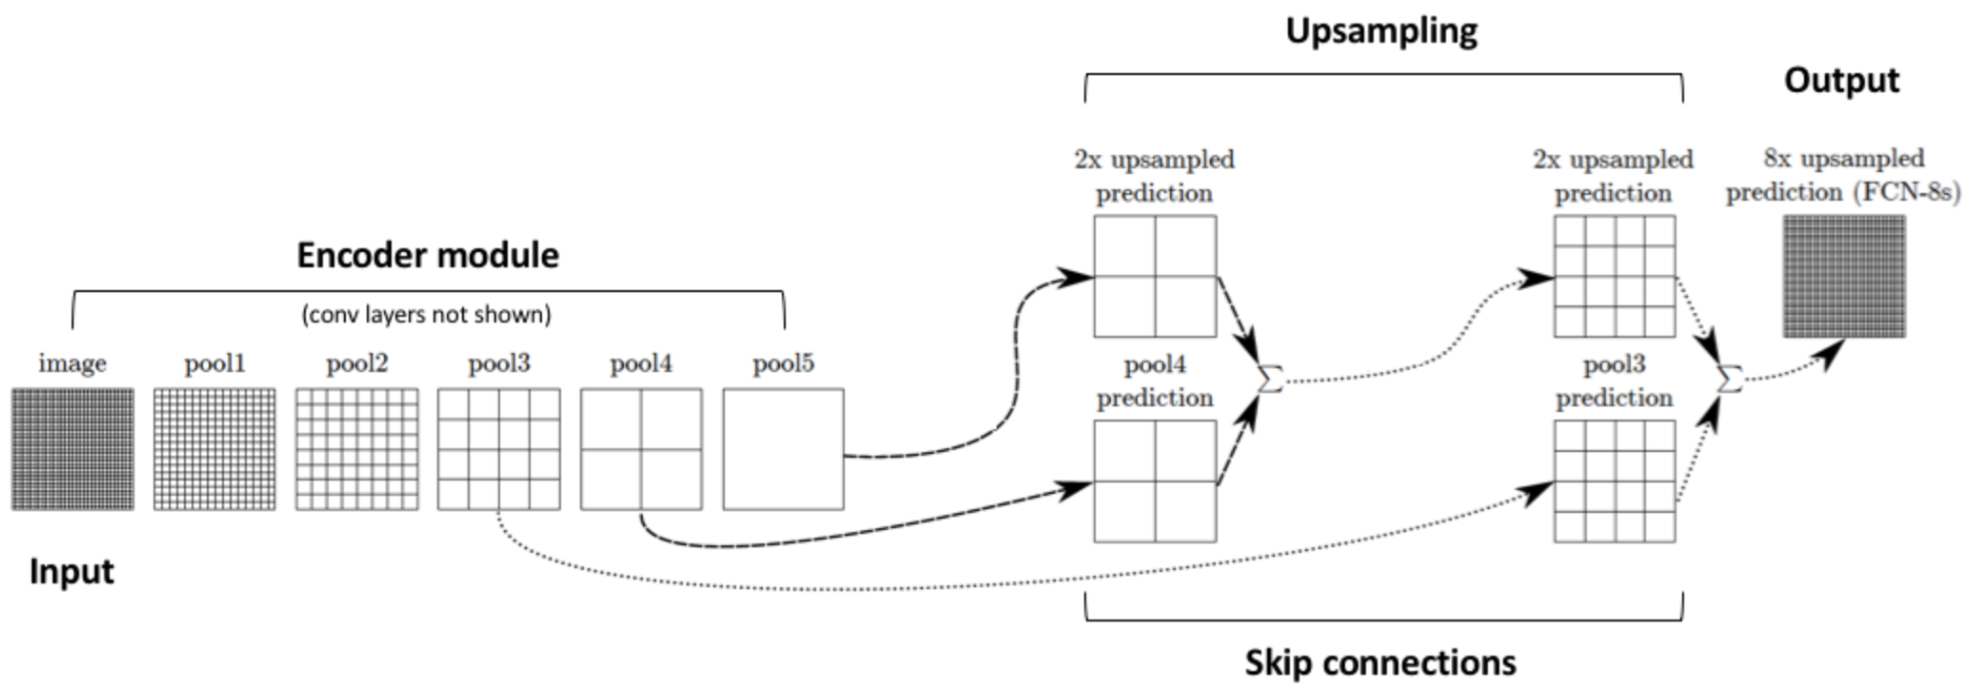
\includegraphics[width=14.5cm, height=4cm]{images/skip_connection.png}
        %\captionof{figure}{The model pipeline.}
        %\label{fig:flow_fig}
\end{minipage} \\

Supplement a traditional "contracting" network by successive layers where convolution is replaced by transpose convolution. \\
Upsampling is ubiquitous and upsampling filters are learned during training. \\
Upsampling filters are initialized using bilinear interpolation. \\
This approach yields 3 networks:
\begin{itemize}
    \item Train first the lowest resolution network (FCN-32s)
    \item Then, the weights of the next network (FCN-16s) are initialized with (FCN-32s)
    \item Tha same for FCN8s
    \item All the FC layers are converted to convolutional layers $1*1$
\end{itemize}{}

Retaining intermediate information is beneficial, the deeper layers contribute to provide a better refined estimate of segments. \\

How to train this network? \\
No need to train patchwise and then transform weights in filters. \\
It is also possible to directly train the whole network on the entire image: 
\begin{itemize}
    \item[--] Define a classification loss in each pixel
    \item[--] Average this loss over the receptive field of each pixel
\end{itemize}{}
Derivative of the sum of the losses can be easily computed and the whole network can be trained through backpropagation. \\
The \textit{patch-based} way:
\begin{enumerate}
    \item Prepare a training set for a classification network
    \item Crop as many patches $\boldsymbol{x_i}$ from annotated images and assign to each patch label corresponding to the path center
    \item Train a CNN for classification from scratches, or fine tune a pre-trained model over the segmentation classes
    \item Once trained the network, move the FC layers to $1*1$ convolutions
    \item Train the upsampling filters
\end{enumerate}{}
The classification network is trained to minimize the classification loss $l$ over a mini-batch: 
$$
\hat{\theta}=\min _{\theta} \sum_{x_{j}} \ell\left(x_{j}, \theta\right)
$$
where $\boldsymbol{x_j}$ belongs to a mini-batch. Batches of patches are randomly assembled during training. It is possible to resample patches for solving class imbalance.\\
It is very inefficient, since convolutions on overlapping patches are repeated multiple times. 

The \textit{full-image} way: 
since the network provides dense predictions, it is possible to directly train a FCNN that includes upsampling layers as well.\\
Learning becomes: 
$$
min \sum_{x_{j}} \ell\left(x_{j}, \theta\right)
$$
Where $\boldsymbol{x_j}$ are all the pixels in a region of the input image and the loss is evaluated over the corresponding labels. Therefore, each path provides already a mini-batch estimate for computing gradient.\\
The full-image way works as follows:
\begin{enumerate}
    \item FCNN are trained in an end-to-end manner
    \item No need to pass through a classification
    \item Takes advantage of FCNN efficiency, does not have to re-compute convolutional features in overlapping regions
\end{enumerate}{}

Drawbacks and solutions: 
\begin{itemize}
    \item[--] Mini-batches are assembled  randomly. Image regions are not. To make the estimated loss a bit stochastic, adopt random mask
    $$
    min\sum_{x_{j}} M\left(x_{j}\right) \ell\left(x_{j}, \theta\right)
    $$
    where $M(\boldsymbol{x_j})$ is a binary random variable
    \item[--] It is not possible to perform patch resampling to compensate for class imbalance: 
    $$
    min \sum_{x_{j}} w\left(x_{j}\right) \ell\left(x_{j}, \theta\right)
    $$
    where $w(\boldsymbol{x_j})$ is a weight that takes into account the true label $\boldsymbol{x_j}$
\end{itemize}{}

\subsubsection{Comments}
Both learning and inference can be performed on the whole-image at-a-time. Both in full-image or batch-training it is possible to perform transfer learning/fine-tuning of pre-trained classification models. \\
Accurate pixel-wise prediction is achieved by upsampling layers.\\
End-to-end training is more efficient than patch-wise training. \\
Being fully-convolutional, this network handles arbitrarily sized input.

%Skip Connection: by summing the two you can take advantage of both this special information and the semantic information that are in the very deep layer. It is the idea of the U-net. You either perform an upsamplig of factor like 32 and then you combine the upsamplig by taking the previous layer and you sum the upsampling and the previous layer.
%In practice you have three network in this way: it start with the one with coarsest resolution so the one with the upsampling of factor 32, then he initializes the factor of 16 with the same weights and all upsampling are initialized by bilinear interpolation. How do you train this sort of network? 
%What you can do is: instead of training the network with a classification loss, you are given all this annotated images with segments where each segment contains a label, you can perform a full-image training which means: given your network, and the output of the network, you can compare the estimated segmentation against the ground truth. The estimated segmentation contains for each pixel a label, the ground truth the same. The loss of your input image is the loss of all your pixels: you obtain a loss for each pixel. 

%The network works besides the image size since it is a fully-connected convolution. 

\subsection{U-Net}
It is the standard for segmentation. The network is composed by a \textit{contracting} part and an \textit{expansive} part, like an encoder-decoder architecture. \\
It takes an image as input, which goes through convolutional layers until the deepest part. Then the upsampling part of the network starts, based on skip connections to get informations of the contracting part. \\
There are no fully-connected layers: there are $L$ convolutions against filters $1*1*N$, to yield predictions out of the convolutional feature maps. \\
The output image is smaller than the input image by a constant boarder. 
Major differences w.r.t. (long et al. 2015): 
\begin{itemize}
    \item use a large number of feature channels in the upsampling part, while in (long et al. 2015) there were a few upsampling. The network become symmetric
    \item Use excessive data-augmentation by applying elastic deformations to the training images
\end{itemize}{}

\begin{wrapfigure}{l}{7cm}
    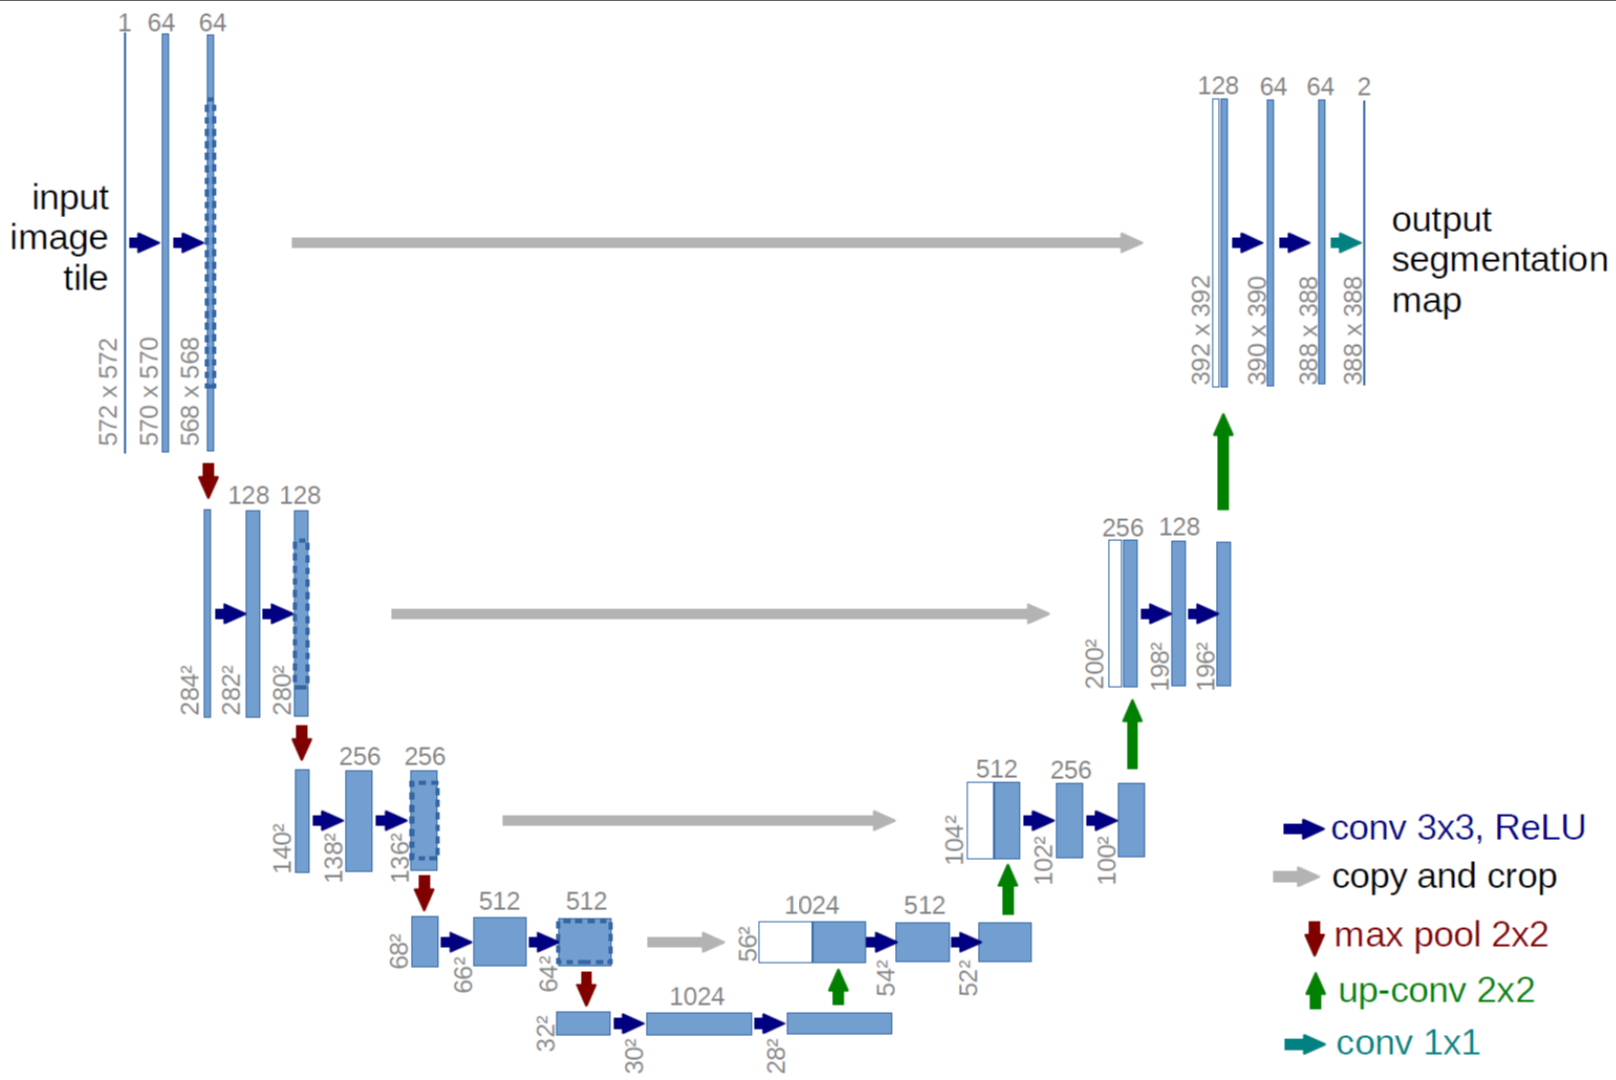
\includegraphics[width=7cm, height=5cm]{images/u_net.png}
    %\label{fig:lstm_org}
\end{wrapfigure}  

The \textit{contracting path}:\\
Repeats blocks of 
\begin{itemize}
    \item[--] $3*3$ convolution + ReLU
    \item[--] $3*3$ convolution + ReLU
    \item[--] Max-pooling $2*2$
\end{itemize}{}
At each downsampling the number of feature maps is doubled

The \textit{expanding path}:
Repeats blocks of:
\begin{itemize}
    \item[--] $2*2$ transpose convolution, halving the number of feature maps
    \item[--] Concatenation of corresponding cropped features
    \item[--] $3*3$ convolution + ReLU
    \item[--] $3*3$ convolution + ReLU
\end{itemize}{}

The main part consists in "aggregation through concatenation + convolution to mix different feature maps in a learnable manner". \\ \\
Training:\\
Full-image training by a weighted loss function:
$$
\hat{\theta}=\min _{\theta} \sum_{x_{j}} w\left(x_{j}\right) \ell\left(x_{j}, \theta\right)
$$
where the weight: 
$$
w(\boldsymbol{x})=w_{c}(\boldsymbol{x})+w_{0} e^{-\frac{\left(d_{1}(\boldsymbol{x})+d_{2}(\boldsymbol{x})\right)^{2}}{2 \sigma^{2}}}
$$
\begin{itemize}
    \item[--] $w_c$ is used to balance class proportions. $w_c(x)$ is a large number for class c that are not very representative in the training set, and it is small for class c that are very representative. 
    \item[--] $d_1$ is the distance to the boarder of the closest cell
    \item[--] $d_2$ is the distance to the boarder of the second closest cell
    \item[--] The first part of the summation takes into account class unbalance in the training set; the second part enhances classification performance at boarders of different objects: in fact, this term is large at pixels close to boarders delimiting object of different classes
    \item[--] For the second term, you have an high weight if the distance  d1 and d2 are large, where d1 and d2 are the distances between the label containing the object and the closest label that is different. Instead when d1 and d2 are small, the weights are small. 
\end{itemize}{}

%Standard for segmentation. The network is composed by a contractive part and an expansive part (encoder and decoder). It takes an image as input, which goes through convolutional layers, until it arrives to the very deepest part. Then the upsampling part of the network starts: what happens is that there are skip connections which brings the information of the contractive part of the network and what is also different is the way this information is been used: when you do upsampling, you have those 2x2 transpose convolution, but you see also that the size is increase by the depth (della parte blu) is halved, this can be done by use fewer filters (here it uses half of the filter). With the transpose convolution, you double the special extent and you copy the output from the corresponding contracting layer and you concatenate it. The upsampling part of the network is a transpose convolution concatenate with the result of the corrisponding contracting layer. In that way the network is able to recover almost the all input(?). At the end of the layer there is no fully-connected layer, it is fully-convolutional. This network is trained in a full-image map so when you measure the loss by average the predictions (forse intende averaging the error?) over the all image. In order to handle the class proportion, you weight your loss in each pixel depending on two factor: 
%\begin{itemize}
%    \item the first $w_c$: balance the class proportion. So $w_c(x)$ is a large number for class c that are not very representative in the training set, and it is small for class c that are very representative. 
%    \item the second $w_0 and so on$: it's mean to improve the classification performance at boundaries of different objects. You have an high weight if the distance  d1 and d2 are large, where d1 and d2 are the distances between the label containing the object and the closest label that is different. So when d1 and d2 are small, the weights are small. 
%\end{itemize}{}

\subsection{Global Averaging Pooling}
\subsubsection{Network in Network}
Introduce two different contributions. When you take a convolutional layer, the output is a linear combination of the inputs. So a linear combination could be too poor approximation to learn. We can use a \textbf{Mlpconv layers}: (Multi-layer-perceptron convolutional layer)
so a fully-connected network over a small portion of the input; 
instead of traditional convolutions, a stack of $1*1$ convolutions + ReLU: $1*1$ convolutions used in a stack followed by ReLU corresponds to a MLP networks used in a sliding manner on the whole image. \\
The same multi-layer perception MLP is used through all the image, this is why MLPconv layer. \\
Each layer features a more powerful functional approximation than a convolutional layer which is just linear + ReLU. \\ 

The other contribution is due to the introduction of \textbf{Global Averaging Pooling} layer: instead of a FC layer at the end of the network, compute the average of each feature map.
\begin{itemize}
    \item[--] The transformation corresponding to GAP is a block diagonal, constant matrix
    \item[--] The transformation of each layer in MLP corresponds to a dense matrix
\end{itemize}{}


\begin{wrapfigure}{r}{7cm}
    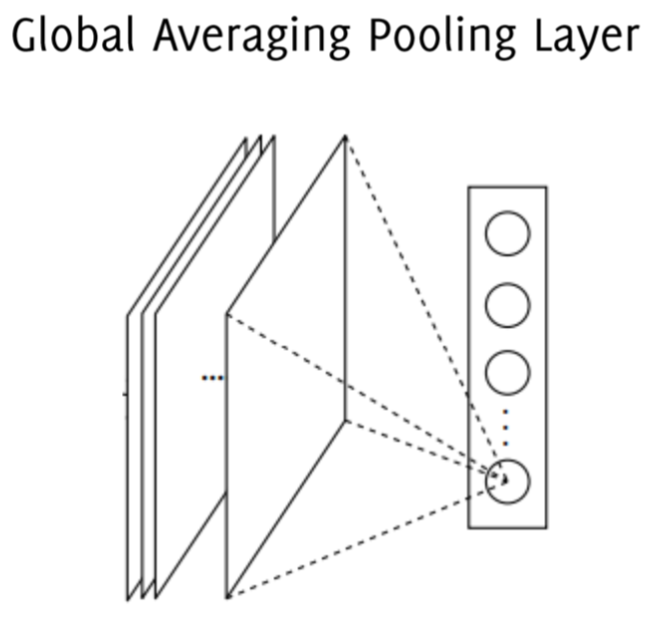
\includegraphics[width=7cm, height=5cm]{images/gap.png}
\end{wrapfigure}  

The reasons behind the introduction of GAP are that \textit{FC layers} are \textit{prone to overfitting}: they have many parameters; the dropout was proposed as a regularized that randomly sets to zero a percentage of activation in the FC layers during training. \\ \\
The GAP strategy instead is \textbf{remove the FC layer} at the end of the network and \textbf{predict by softmax} after the GAP. \\
The advantages of Global Averaging Pooling Layers:
\begin{enumerate}
    \item No parameters to optimize, lighter network less prone to overfitting
    \item More interpretability, creates a direct connection between layers and classes output
    \item This makes GAP a structural regularizer
    \item More robustness to spatial transformation of the input images
    \item The network can be used to images of different sizes
\end{enumerate}{}
Classification is performed by a softmax layer at the end of the GAP.

%Global Averaging Pooling
%Network in Network: introduce two different contribution. When you take a convolutional layer, the output is a linear combination of the inputs. So what they say is that a linear combination is too poor approximation to learn a network. What he should do is instead of having a convolution, he uses a multilayer perceptron network, so a fully-connected network over a small portion of the input and then he uses the same multi-layer perceptron through all the image. Instead of using a convolution as a filter, he uses a small multi-layer perceptron. This is called Multi-Layer Perceptron Convolutional layer (MLPconv layer) because the same multi-layer perceptron is used through all the network in a convolutional way. 

%The second point he propose is Global Averaging Pooling: it's another way to handle the fact that images may have different size; the all values over a slice here, in the deepest activation of the network, and out of all this values it simply compute the average. It takes the second slice and compute the average. At the end you have to compute the softmax over this vector of averages. If you are not interest in segmentation, what you can do when you get to the final layer of the network, you can compute the average of each layer and use the vector of the average as vector representation. 

%So the biggest advantage is that you get rid of fully-connected layer, the one with more parameter and the more prone to overfit. What was propose in the literature is to introduce dropouts between the hidden layers of the multi-layer perceptron network, as a regularizer. 

%slides 'this makes GAP a structural regualrizer': because you got less parameters and your estimate becomes less dependent on the location of a certain feature in the image, because you completely ignore the spatial extent while performing the predictions. So you have more robustness (continuare sulle slides)


\section{Localization and Object Detection}
\subsection{Localization}
The input image contains a single relevant object to be classified in a fixed set of categories. The task is:
\begin{itemize}
    \item Assign the object class to the image
    \item Locate the object in the image by its bounding box
\end{itemize}{}

The task is a prediction task which involve a discrete output and 4 different outputs which are the bounding box limits. 

\subsubsection{Simplest Solution}
The network have to be both a \textit{classification} network and a \textit{regression} network to identify bounding boxes, so you need to combine two different losses. The training loss has to be a single scalar since we compute gradient of a scalar function w.r.t. network parameters. The idea is to minimize a multitask loss to merge two losses:
$$
\mathcal{L}(x)=\alpha \delta(x)+(1-\alpha) \mathcal{R}(x)
$$
where the hyper-parameter $\alpha$ is used to balance the losses to make the two losses in a similar range. Watch out that $\alpha$ directly influences the loss definition, so tuning might be difficult, better to do cross-validation looking at some other loss.\\
So you will have \textit{two different ends} of your network, one part with $L$ (number of classes) neurons, and the other will predict the 4 bounding boxes. \\ \\
Human-Pose Estimation is formulated as a \textbf{CNN-regression problem} towards \textit{body joints}. The network receives as input the whole image, capturing the full-context of each body joints.
The approach is very simple to design and train. Training problems can be alleviated by transfer learning of existing classification networks. 
Pose is defined as a vector of $k$ joints location for the human body, possibly normalized w.r.t. the bounding box enclosing the human. 

\subsubsection{Weakly-Supervised Localization}
Perform localization over an image without any annotating bounding box. So you train your network as a classification network to assign to each image a label, but you want also your network to perform localization. The only form of supervision is the classification label, not the bounding box: only the classification labels are provided.\\ \\
This is a sort of Global Averaging Pooling \textit{revisited}: the advantages of GAP layer extend beyond simply acting as a structural regularizer that prevents overfitting; in fact, the network can retain a remarkable localization ability until the final layer. By a simple tweak it is possible to easily identify the discriminative image regions leading to a prediction.\\
\begin{quote}
    \textit{A CNN trained on \textbf{object categorization} is successfully able to localize the discriminative regions for action classification as the object that the humans are interacting with rather than the humans themselves}
\end{quote} 

Your network takes in input an image and provides a big volume. The larger of image, the larger the volume is. In case of classification, you have to squeeze down this volume to a fixed size, which is the input of the fully connected layer. \\
An option is to \textit{resize} the image, the other option is to introduce another \textit{GAP layer}: average the values of each slice of the volume. So you have a vector with a value for each one of the $n$ slices and, at the end, what you get is a vector of length $n$. \\
\textit{GAP} is shown to perform better in some cases than Dropout in order to perform Regularization. This is why it is useful, it's \underline{reduce overfitting} and can be used with \underline{images of any shape}. 

\begin{wrapfigure}{l}{6cm}
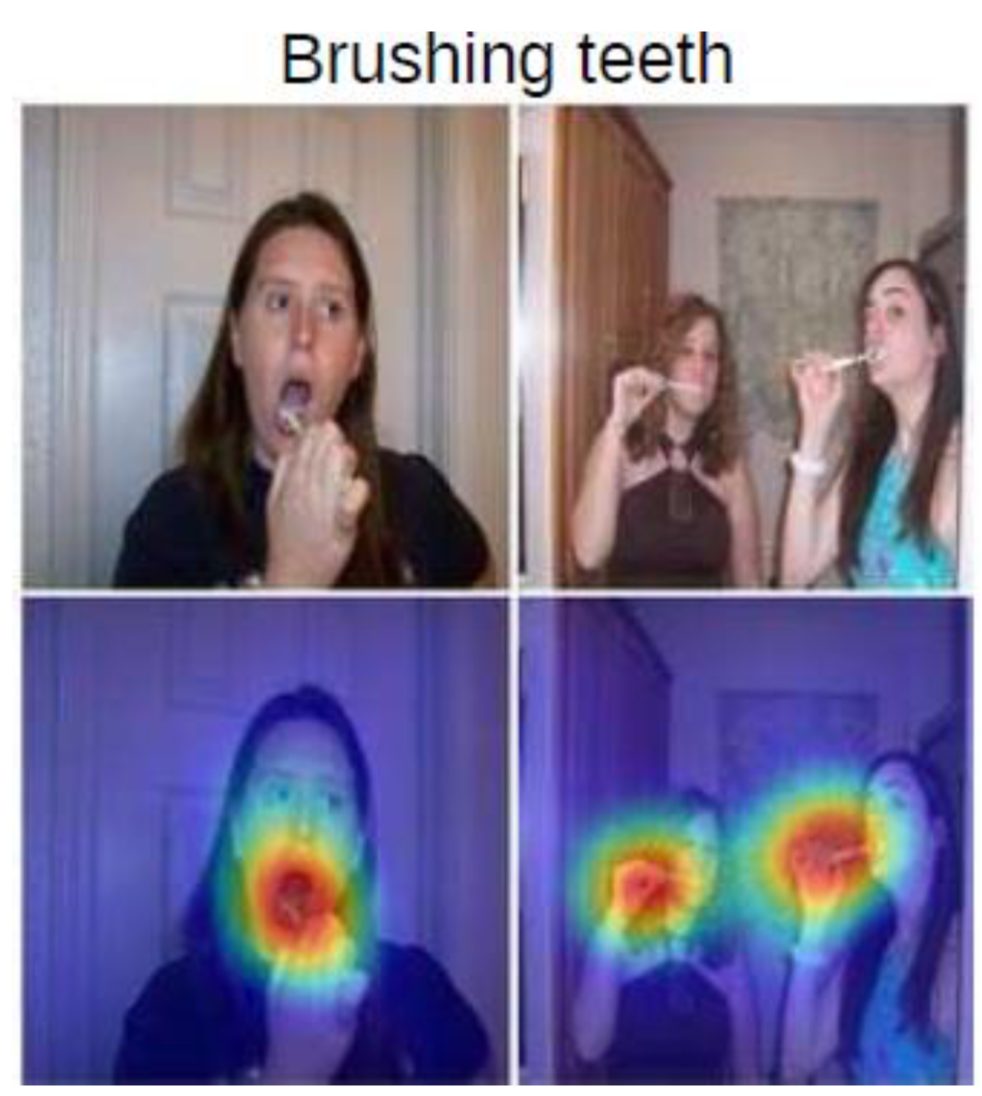
\includegraphics[width=5cm]{images/heatmap_localization.png}
\caption{Heatmaps}\label{wrap-fig:heatmap_loc}
\end{wrapfigure} 

In the paper, GAP it is also presented as a tool to modify slightly your network and get instead a classification network, a network that perform a sort of Localization: it is able to localize discriminative regions for the classification task at the object that human are interactive with. In fact, the heatmaps show which is the image region which has mostly influenced the network decision. This kind of heatmap is perfect to identify bounding boxes. 

The nice part of the story is that if you take any classification network, you introduce a GAP layer, you get for free a network that is able to provide that sort of heatmap, so you are able to perform Localization. \\ \\
This approach of identifying exactly which regions of an image are being used for discrimination is called \textbf{Class Activation Map}: it is very easy to compute since it just requires an FC layer after the GAP and a minor tweak. \\

 \begin{wrapfigure}{r}{7cm}
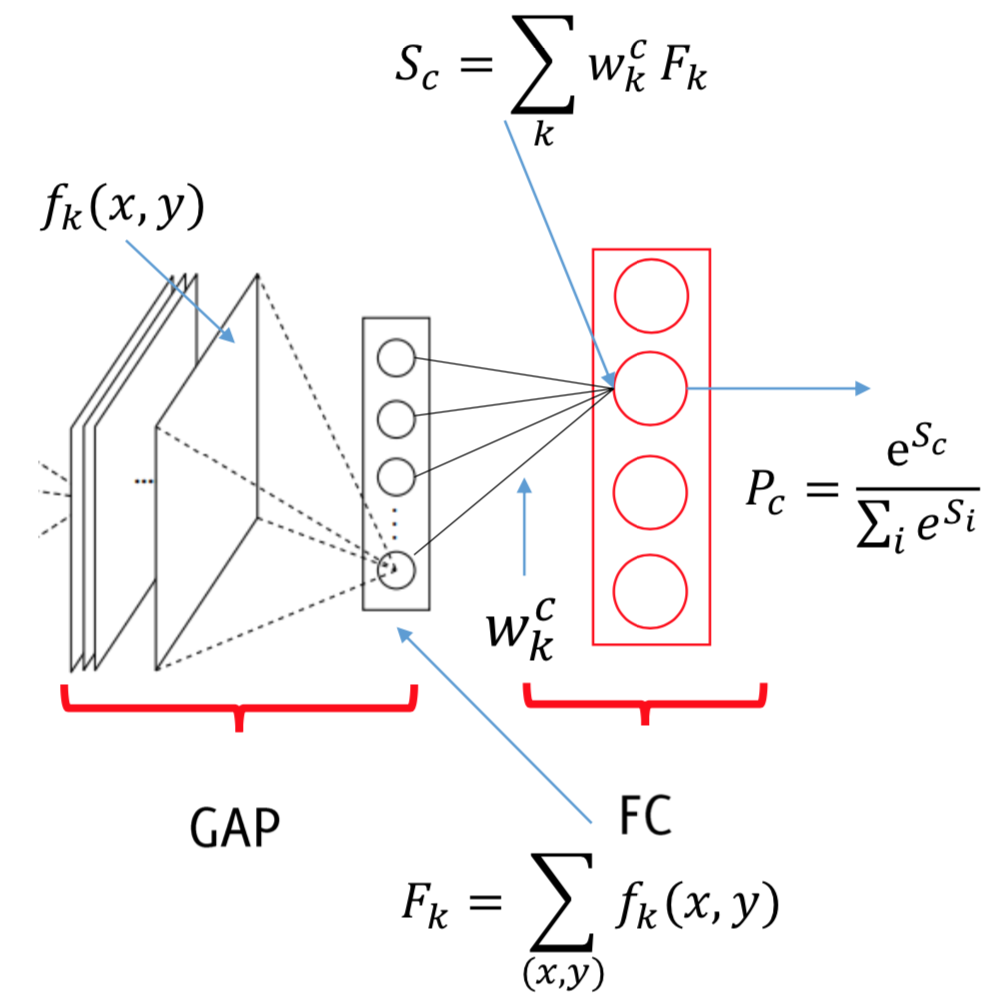
\includegraphics[width=7cm]{images/GAP_layer.png}
\caption{GAP layer}\label{wrap-fig:gap_layer}
\end{wrapfigure} 

Considering Fig.\ref{wrap-fig:gap_layer}, a very simple architecture made only of convolutions and activation functions leads to a final layer having: 
\begin{itemize}
    \item[--] $n$ feature maps $f_k(:,:)$ having resolution "similar" to the input image
    \item[--] a vector after GAP made of $n$ averages $F_k$
\end{itemize}
The FC layer after the GAP it's the output layer which computes $S_c$ for each class $c$ by the weighted sum of {$F_k$}, where weights $w_k^c$ are defined during training. Then, we can extract the class probability $P_c$ via softmax, for each class $c$. The weights $w_k^c$ encodes the importance of $F_k$ for the class $c$ 
$$
S_c = \sum_{k=1}^{N} w_k^{c}F_k = \sum_{k=1}^{N} w_k^{c} \sum_{x,y} f_k(x,y) = \sum_{x,y} \sum_{k} w_k^c f_k(x,y)
$$
\\ \\
%after the last part of convolution of the network, we perform a GAP and we get a vector of size $n$, where $n$ is the number of slices of the last convolutional layer. We call $F_1$ the average of the fist slice, $F_2$ the average of the second layer and so on. Now you can just introduce a simple output layer, so in case of a classifier, you have a fully-connected layers with n neurons. So once you train, you have multiple weights $w_1$, $w_2$ and so on. When you feed an image, you can take the softmax to obtain the predicted class; then you can take the weights: let's call the weights $w_{i}^c$, where c defines the specific class and i the i-th value, and the score is:

So you can construct an image where in each pixel there is the linear combination of all the weights corresponding to a slices rescaled by the corresponding weighth $w_k^c$. The image in the output is exactly the heatmap which highlights which part of the image contributes more on the decision of the network. The results is called Class Activation Map which is defined as:
$$
M_{c}(x, y)=\sum_{k} w_{k}^{c} f_{k}(x, y)
$$
where $M_{c}(x, y)$ directly indicates the importanc of the acrivations at $(x,y)$ for predicting the class $c$. Thanks to the softmax, the depth of the last convolutional volume can differ from the number of classes. 
%linear combination between all the slices * the corresponding weight.

%Important: slide 18: dando in input l'immagine, più passa per la convoluzione, più il blocco di convoluzione diventa piccolo. Per farlo tornare alla grandezza dell'immagine in modo da avere delle heatmap della stessa grandezza dell'immagine di input, dobbiamo fare upsampling. Un'altra opzione sarebbe quella di fare una sorta di U-net come la segmentation, si ottiene più resolution ma less semantic. \\
When we feed the CNN with an input image, we get a convolutional block (the volume) which becomes smaller as the input pass through the network. We need to perform an upsampling to obtain the an heatmap of the same size of the input image. Another option would be to perform a sort of U-net as the segmentation problem, obtaining more resolution but less semantic. \\
As shown in Fig.\ref{fig:cam}, the weights represents the importance of each feature map to yield the final prediction.

 \begin{figure}[h]
    \centering
    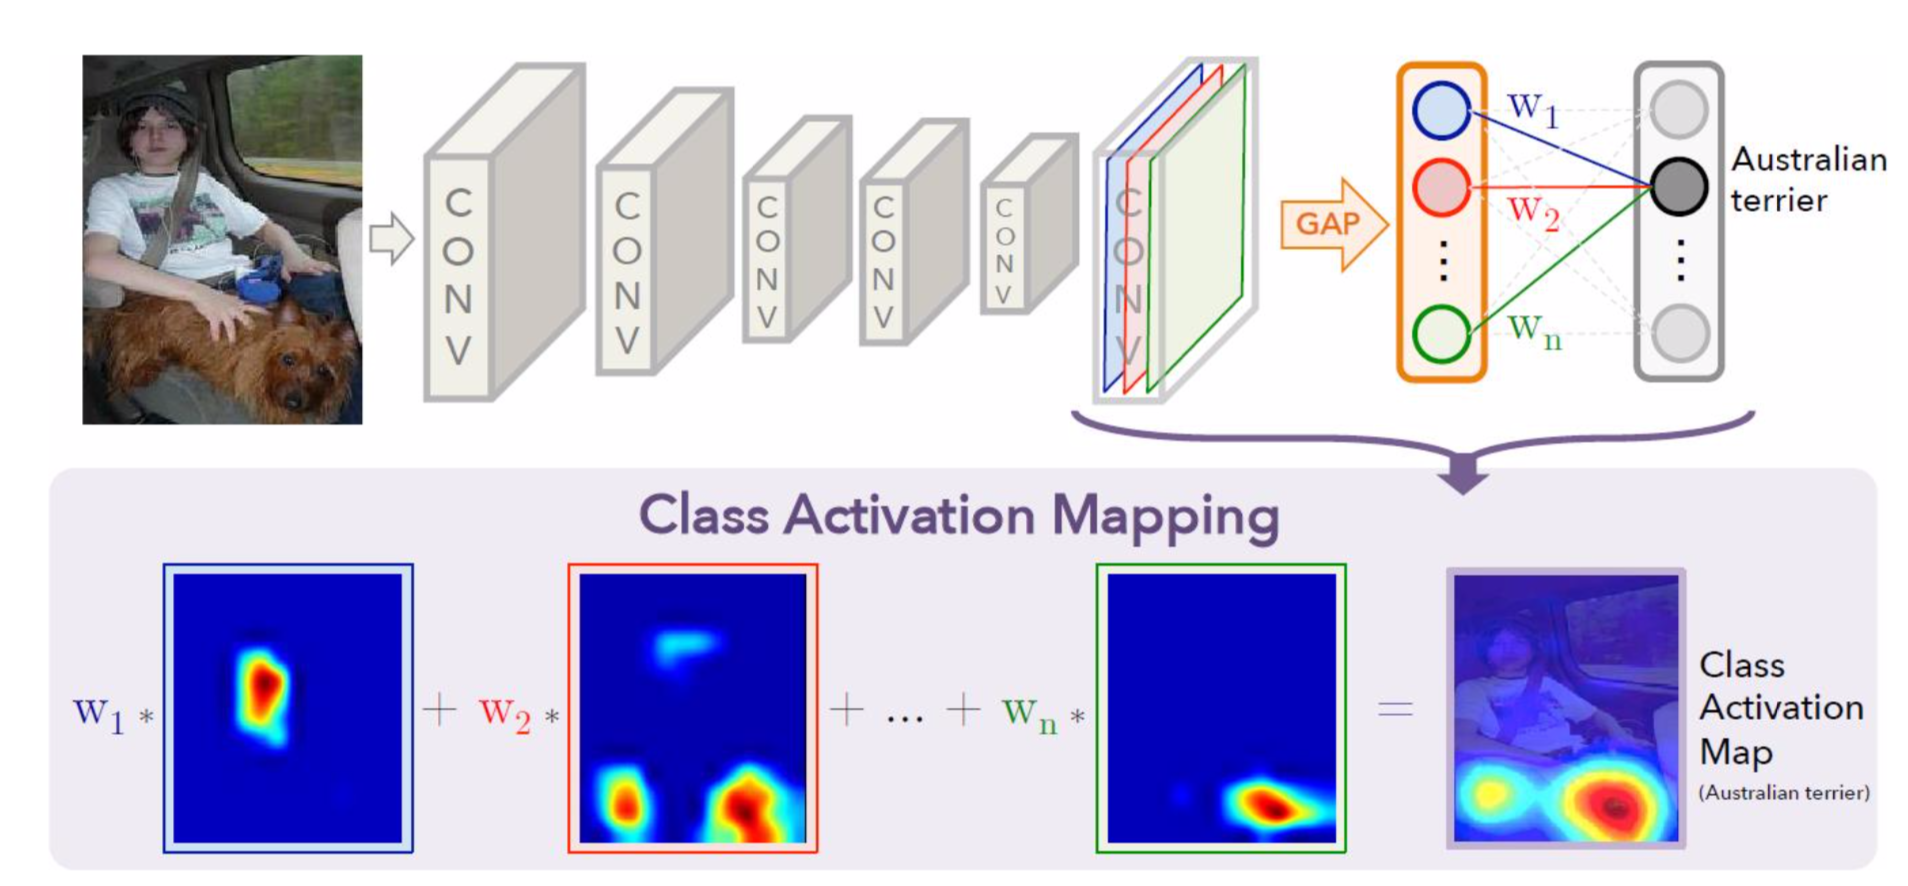
\includegraphics[width=15cm, height=6cm]{images/cam.png}
    \caption{Class Activation Map}
    \label{fig:cam}
\end{figure}
%(quando si mette una fully-connected si aumentano tantissimo i parametri quindi le performance cadono drasticamente).
\textbf{Remarks}:
\begin{itemize}
    \item[--] CAM can be included in any pre-trained network, as long as the FC layer is removed
    \item[--] The FC used for CAM is simple, few neurons and nohidden layers
    \item[--] Classification performance might drop (in VGG removing FC means loosing 90\% of  parameters)
    \item[--] CAM resolution (localization accuracy) can improve by "anticipating" GAP to larger convolutional feature maps
    \item[--] GAP: encourages the identification of the whole object, as all the part of the values in the activation map concurs to the classification 
    \item[--] \textbf{GMP} (\textbf{Global Max Pooling}): it is enough to have a high maximum, thus promotes specific discriminative features
\end{itemize}{}

The fully-connected part of the network is very simple, but it requires changing the network and loosing performance (adding a fully-connected layer drops the performance).\\ \\
\textbf{Grad-CAM} computes that weights to the gradient of back propagation, you don't even have to change the network (a fully-connected network at the end is not required) and it is good because if you get a pre-trained network for doing other stuff (captioning, object detection) you don't have to change it. You can use these heatmaps even attaching them to an existing network without the need to retrain them. 

\subsection{Object Detection}
Given a fixed set of categories and an input image which contains an unknow and varying number of instances, draw a bounding box on each object instance. A training set of annotated images with label and bounding boxes for each object is required. Each image might require a different number of outputs, depending on the number of object detected. \\ \\

In fact, the tricky part is that the number of output is not pre-defined, it depends on the input image. \\
Different solutions are proposed:

\subsubsection{Sliding Windows}
Define a certain patch (a sort of box that captures a portion of the image) size and slide this patch on the image, classify the content in that patch. If you get some output with high probability then you might take that as output of your object detection algorithm. \\
A pre-trained model is meant to process a fixed input size, so you have to slide on the image a window of that size and classify each region, assigning the predicted label to the central pixel.
There is a special class that is 'background' which means that there is no relevant object inside that patch. \\
It is very inefficient since for identify an object, e.g. a car, entirely you need a bigger bounding box. So theoretically you have to test different patch size. It does not re-use features that are "shared" among overlapping crops.  Inefficient also if you consider only a single patch size: take a patch and slide means compute convolution multiple times for each pixel because each pixel belongs to multiple patches. Moreover, each patch feeds the network independently from the others and all the operation are repeated multiple times. 
The only advantage is that there is no need of retraining the CNN.

\subsubsection{Region Proposal}
Region Proposal algorithms (and networks) are meant to identify bounding boxes that corresponds to a candidate object in the image.\\ \\
The first network performing object detection were actually based over these techniques. These algorithms have an high recall (if there is an object, those algorithms provide a bounding box), but very low precision because they provide a lots of region proposal out of a image.\\
The idea is: apply a region proposal algorithm $\rightarrow$ Classify by a CNN the image inside each proposal regions

\subsubsection{R-CNN: Region-CNN}
Object detection by means of region proposal. So given an input image, run the Region Proposal algorithm and extract a huge amount of proposals, e.g.. 2K of proposals. Modify the content of your region proposal to become a square since  the network is a standard CNN which expects a fixed input size. \\ \\
Taking the cowboy image, once extracted the regions, you squeeze the cowboy to be a square. The major drawback is that in this way you lost the proportion, relevant to understand the content. \\

 \begin{figure}[h]
    \centering
    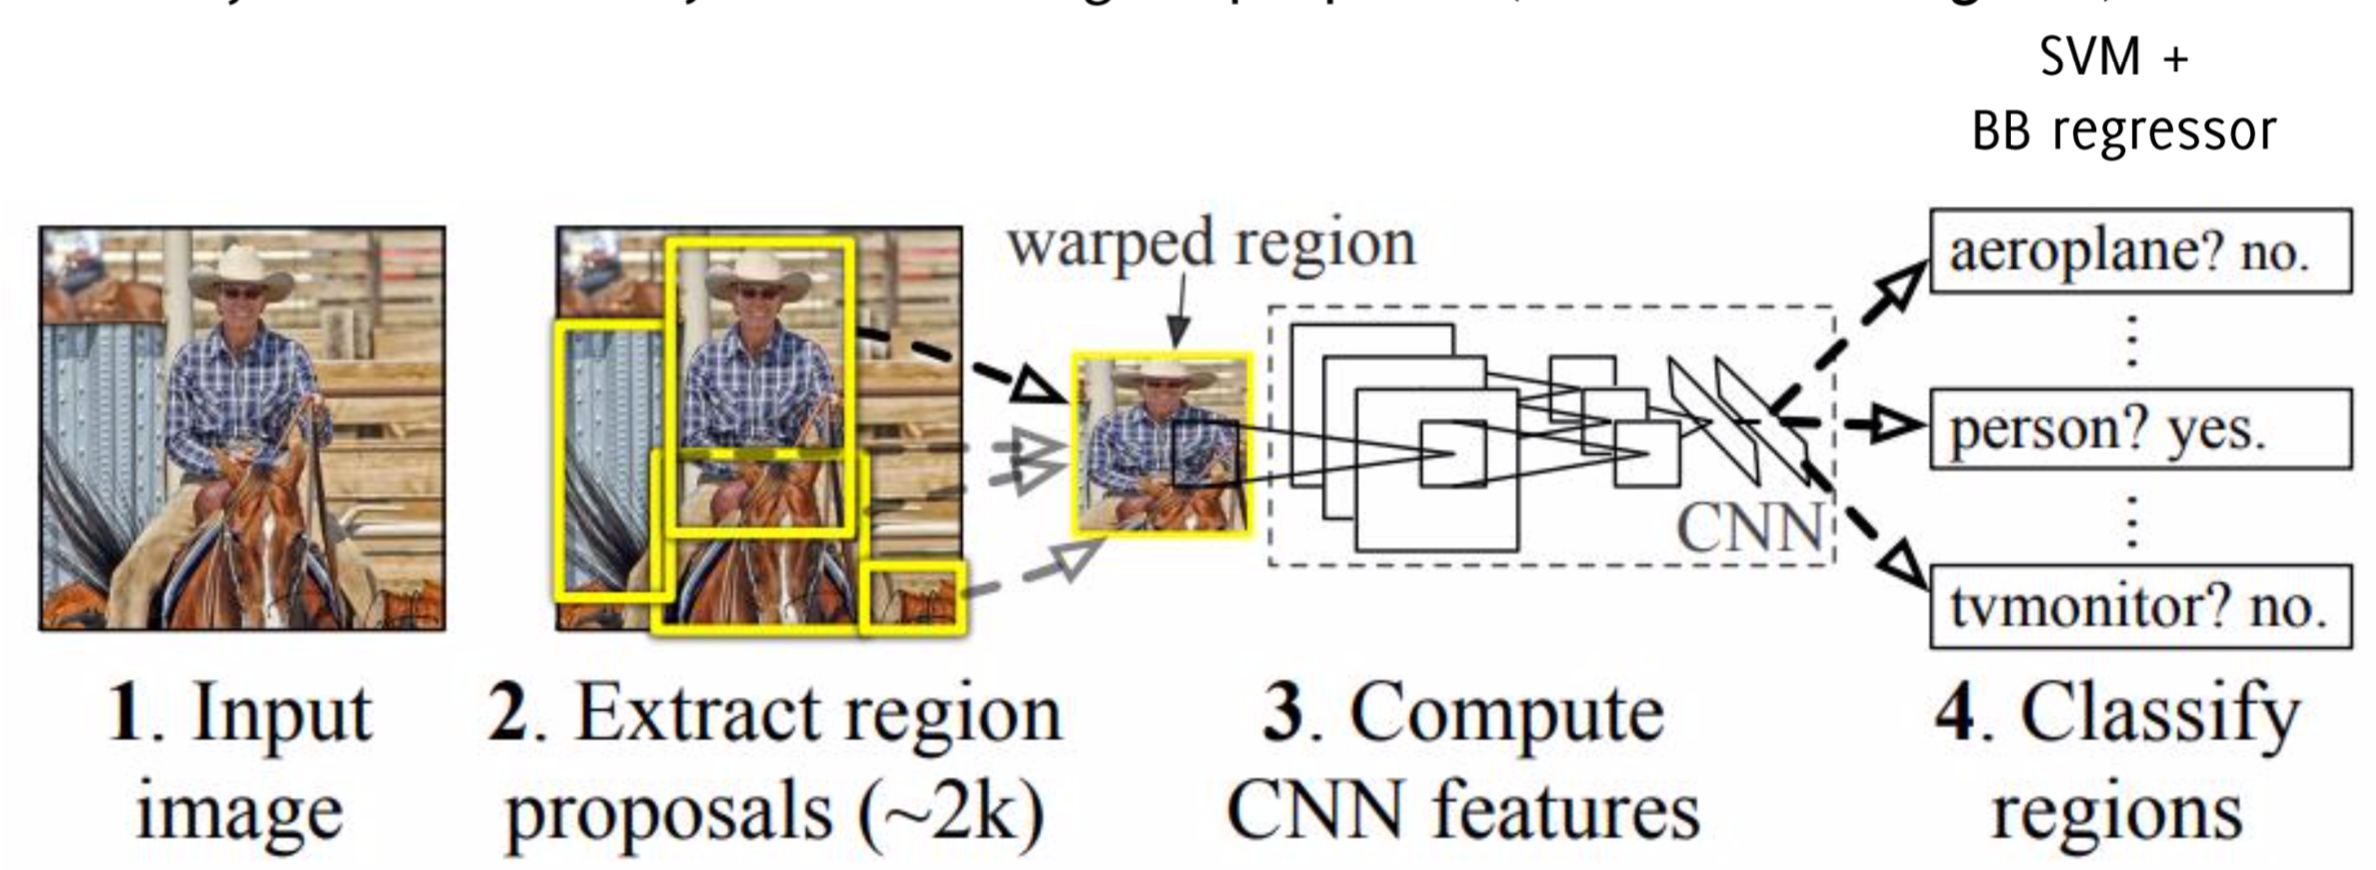
\includegraphics[width=15cm, height=6cm]{images/r_cnn.png}
    \caption{R-CNN}
    \label{fig:r-cnn}
\end{figure}

So Region Proposal detects the input, CNN extracts the features. At the end it is used a SVM in order to classify and find out what will be the label of the region proposal. On top of that, a bounding box regression in order to improve the localization, so there will be different losses. \\
There was no learning algorithm in the Region Proposal, so a very high recall. Instead, the CNN is fine-tuned during training. \\
However, this architecture has some limitations: 
\begin{itemize}
    \item[--] Ad-hoc training objectives and not an end-to-end training: fine-tune network with a softmax classifier, train post-hoc linear SVMs, train post-hoc bounding-box regressions
    \item[--] \textbf{Region proposal are from a different algorithm} (Region Proposal) and that part has not been optimized for the detection by CNN
    \item[--] Training is \textbf{slow}, you get a lot of proposal and for each of them you have to extract the features by the CNN $\rightarrow$ takes a \textbf{lot of disk space} to store features. 
    \item[--] \textbf{Inference is slow} since the CNN has to be executed on each region proposal (\textbf{no feature re-use})
\end{itemize}{}

\subsubsection{Fast R-CNN}
To save a lot of time, especially in inference time, instead of cropping the regions on the image and passing the image, cropped and resized, to another network, you can just \textbf{project the region proposals} from the input image over the last fully-convolutional layer: you have to perform all the CNN just once. 

 \begin{figure}[h]
    \centering
    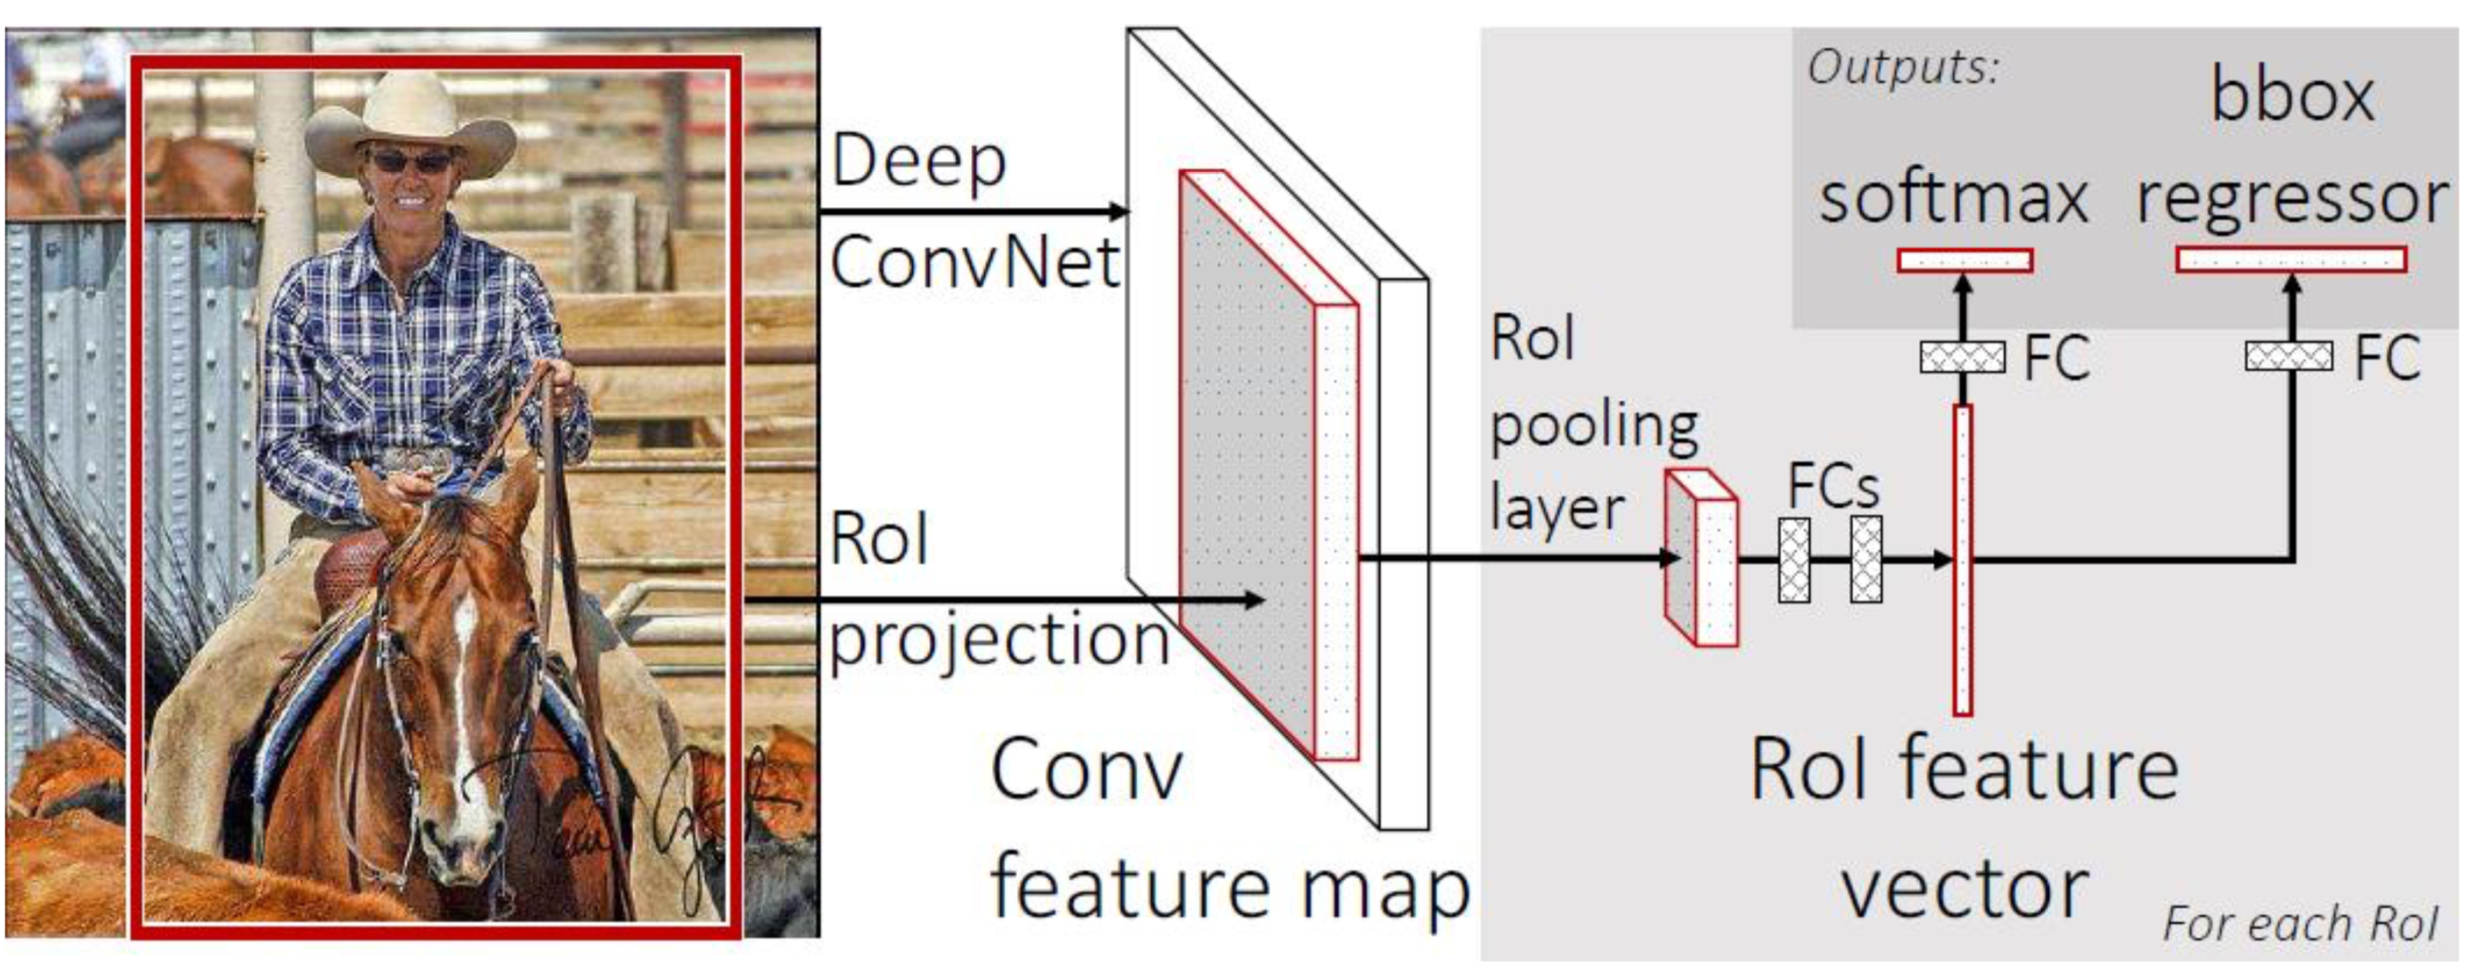
\includegraphics[width=15cm, height=6cm]{images/fast_r_cnn.png}
    \caption{Fast R-CNN}
    \label{fig:fast-r-cnn}
\end{figure}

%So you feed the image to a big CNN and the same image to a Region Proposal Algorithm. The latter returns a lot of regions, which are not used to extract a portion of the image, resized it and fed to a CNN, but you simply project this regions over the last fully-convolutional layer of the network.
%You don't have to crop and feed the same image 2000 times the same image, you have just to extract the regions and project them to the last layer. 

\begin{enumerate}
    \item The wholw image is fed to a CNN that extracts feature maps
    \item Region proposal are identified from the image and progected into the feature maps. Regions are directly cropped from the feature maps, instead from the image $\rightarrow$ re-use convolutional computation
    \item Fixed size is still required to feed data to a fully connected layer. \textbf{ROI Pooling layers} extract a feature vector of fixed size $HxW$ from each region proposal. Each ROI in the feature maps is divided in a $HxW$ grid and then max-pooling over this provides the feature vector
    \item The FC layers estimate both classes and BB location (BB regressor). A convex Combination of the two is used as a multi-task loss to be optimized (as in R-CNN, but no SVM here)
    \item Training in an end-to-end manner
\end{enumerate}{}

Some issues: here you are using this network only to extract features; once you have these feature and you have to feed an architecture with them for classification, you have to fix the  input size. So the problem has been postponed: what Ross (the creator of Fast R-CNN) does is \textit{ROI Pooling layer}: whatever partial size the projected region proposal has, you divide it in $HxW$ blocks and you perform max pooling on these regions. \\
What you get is a volume with a fixed special extent: it's like max pooling which works on larger neighbours if the regions are larger, and smaller vice-versa. \\
Still the cowboy is squeezed but it is \textit{squeezed on the features} and with the max pooling. Then you can predict the class and the bounding box location (softmax and BBox regressor). \\ \\

By doing this you can \textit{backpropagate this loss through the whole network}, which becomes incredibly faster than R-CNN during testing. Now that convolutionss are not repeated on overlapping areas, the vast majority of test is spent on ROI extraction: most of inference time is spending on extracting Region Proposal.

\subsubsection{Faster R-CNN}
Faster R-CNN gets close to real-time object detection. You move Region Proposal inside the network: you train a network in order to extract the convolutional features, from them you extract a region proposal. You do not look at the image anymore, you look at the feature map directly. \\ 

Instead of the ROI extraction algorithm, a region proposal network (\textbf{RPN}) is used in order to extract a region proposal from the convolutional features. So RPN operates on feature maps of the last convolutional layers. The remaining operation are very similar to a Fast R-CNN \\ 

You feed your CNN with an input image, you get a volume (the convolutional features) and there you run RPN. \\ 
The Region Proposal network works as follows: it takes a filter of $3x3$ and slide the feature maps. It maps (by 1x1 convolution) the region to a lower dimension vector. In each point it consider $k$ anchor boxes, i.e. different ROI size/proportions (k-possible templates for region), thus there  $HxWxk$ candidate anchors.\\
The classification network (\textit{cls} network) is trained to predict the object probability, i.e. that each anchor contains an object \textit{[obj, no-obj]} $\rightarrow$ $2k$ probability estimates.  
The region network (\textit{reg} network) is trained to adjust the anchor to the object ground truth $\rightarrow$ $4k$ estimates.\\
There is no need to design different RPN to account for the $k$ different anchors. \textbf{Anchors just influence the way labels of RPN are comuted}. \\
Training now involves 4 losses: RPN classify object/non-object, RPN regression coordinates, final classification score, final BB coordinates. During the training, object/non-object ground truth is defined by measuring the overlap with annotated BB. \\
The network becomes much faster also because you don't have to design a different network for each shape of region proposal, you just train the network to predict for each of these $k$ different outputs, which correspond to an object in the image. \\
At test time:
\begin{itemize}
    \item Take the top ~300 anchors according to their object scores
    \item Consider the refined boundig box location of these 300 anchors
    \item These are the ROI to be fed to a Fast R-CNN (ROI pooling to perform the downsampling)
    \item Classify ROI
\end{itemize}{}
Therefore, Faster R-CNN provides to each image a set of BB with their objectness score.\\
It's still a \textbf{two stage detector}, where in the first stage:
\begin{itemize}
    \item run a backbone network (e.g. VGG16) to extract features
    \item run the Region Proposal network to estimate circa 300 ROI
\end{itemize}{}

In the second stage (the same as in Fast R-CNN):
\begin{itemize}
    \item Crop features through ROI pooling (with alignment)
    \item Predict object class using FC + softmax
    \item Predict bounding box offset to improve localization using FC + softmax
\end{itemize}{}
%for each location, where $HxWxk$ is the special extent of this volume, you consider 3x3 regions in the feature map, so 3x3xN. It performs a one-by-one convolution to reduce the size of the image. So you get a vector reduced representation of 256-dimension and out of this vector you perform a regression over different location in order to determine where there is a region there. So in particular you have k-possible templates for region. For each pixel, you take a subvolume, you map it in a 256-dimensional vector and you have a prediction where this is the location of k different region proposal which are of different proportion. So you train your network to predict HxWxk possible shapes for the region proposal. You don't have to design a different network for each shape of region proposal, you just train the network to predict for each of these k different outputs, which correspond to an object in the image.
%So the network is predicting whether in each point in the feature map there is one of those k possible bounding boxing. 
%To train it, you need 4 different losses: 1 classify the object, 1 for the regression of the coordinates, 1 to classify the final classification score and the final bounding box score. 
%This allows you to take at test time 300 most probable bounding boxes (anchor points), then consider only these 300 as candidate location for an output and once you have them, you feed them to the first network. The rest is the same: ROI pooling to perform the down sampling and then you classify them. 
%It is a two stage detector. 
%This provides an incredible speed-up. 

\subsubsection{You Only Look Once (YOLO)/ Single Shot Detectors (SSD)}
R-CNN methods are based on Region proposal, but there are also region-free methods, like YOLO or SSD. Detection networks are indeed a pipeline of multiple steps. In particular, region-based methods make it necessary to have two steps during inference. This can be slow to run and hard to optimize, because each individual component must be trained separately.\\ \\
In YOLO 
\begin{quote}
    \textit{We reframe the object detectino as a single regression problem, straight from image pixels to bounding box coordinates and class probabilities}
\end{quote}{}
And solve these regression problems \textbf{all at once}, with a large CNN. \\
These algorithms don't have to go to this two stage phases, they cast all the object detection as bounding box regression problem, starting from the image. \\

In YOLO: 
\begin{enumerate}
    \item Divide the image in a coarse grid
    \item each grid cell contains $B$ \textit{base-bounding boxes} associated
    \item For each cell and \textit{base-bounding box} we want to predict: 
    \begin{itemize}
        \item the offset of the base bounding box, to better match the object: (dx, dy, dh, dw, objectness score)
        \item The classification score of the base-bounding box over the $C$ considered categories (including background)
    \end{itemize}{}
\end{enumerate}{}

The whole prediction is performed in a single forward pass over the image, by a single convolutional network. Training this network is sort of tricky to assess the loss (matched/not-matched).\\
YOLO/SSD shres a similar ground of the RPN used in Faster R-CNN. Typically networks based on region-proposal are more accurate, single shot detectors are faster but less accurate.
%you crop the image on a grid; inside of each it propose a anchor, so a candidate location for a possible region proposal and then train a network which is meant to determine whether each of this region can be the location for an object and the corresponding bouding box. 
%This part is sort of similar as the Faster-R-CNN. This is like one-shot. 

\section{Standard Architectures for Image Classification}
We are talking about networks for image classification. 
\subsection{GooglLeNet and Inception v1}
This is the network that won the competition in 2014 achieving a classification error of 6.7\%.
It is composed of the so called inception modules. The basic idea of the model is this:
\begin{center}
    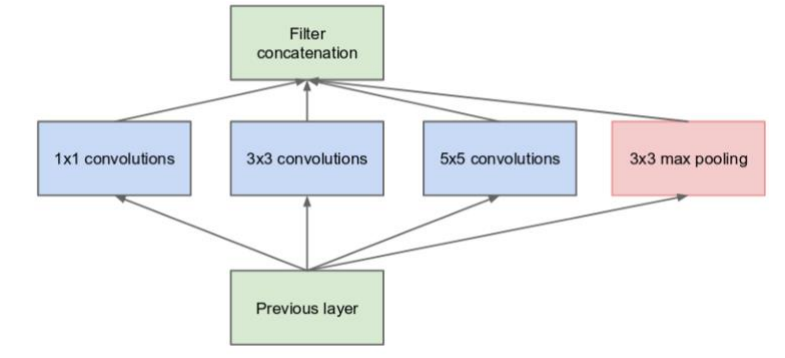
\includegraphics[width=0.7\textwidth]{images/googlenet.PNG}\par
\end{center}
A volume enters not a convolutional layer but in parallel multiple convolutional layers and a max pooling layer. Then all these outputs are combined together by concatenation to produce the layer output. There are multiple filter sizes in this way. The idea is that this was a sort of solution basing on the fact that it's hard to choose the filter size for feature extraction. 

Assuming you have a very small volume of 28x28x256, you perform some convolution (depending of the number of filters you will obviously have different numbers) with 128 filters 1x1, 192 3x3, 128 5x5 and 256 3x3 max pooling. To concatenate the output you perform some zero padding to preserve the spatial size, but the depth is increased. There are a large number of operations to be performed due to the large depth of the input of each convolutional layer (858 millions in this example). This is too expensive to compute, this network is expanding its depth preserving the spatial extent. To reduce the computational demand we can use the 1x1 convolution: we can stack 1x1 convolutional blocks right before 3x3 and 5x5 and after the max pooling. These 1x1 blocks are used as \textit{bottleneck layers}, in order to compress the number of features and create another non linearity. 
\begin{center}
    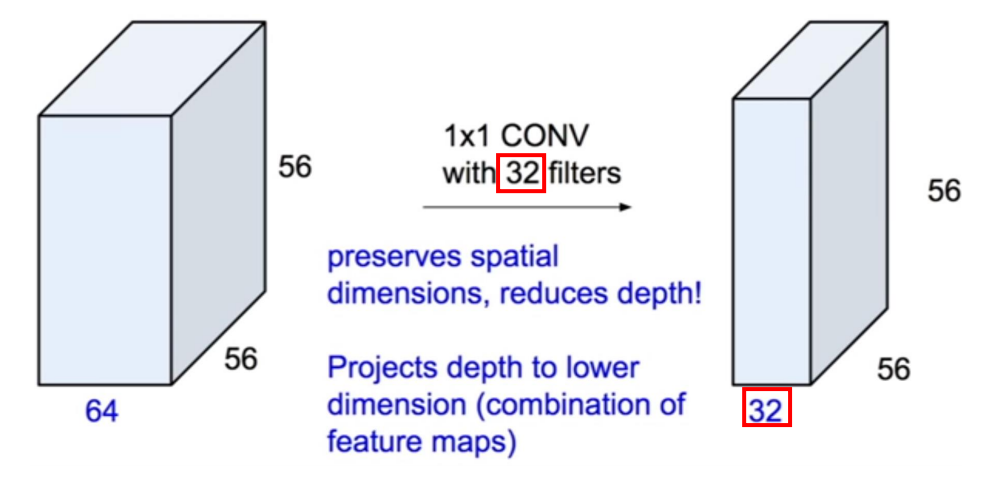
\includegraphics[width=0.6\textwidth]{images/1x1conb.PNG}\par
\end{center}
If you take 32 of these 1x1 filters, the output will have size 32 because each 1x1 filter will pass through the image providing one slice of the output. In this way the number of operations is significantly lower. There are overall 27 layers made of 9 inception modules; at the end you don't need a fully connected layer, there's only a global averaging pooling, a linear classifier and a softmax.
\begin{center}
    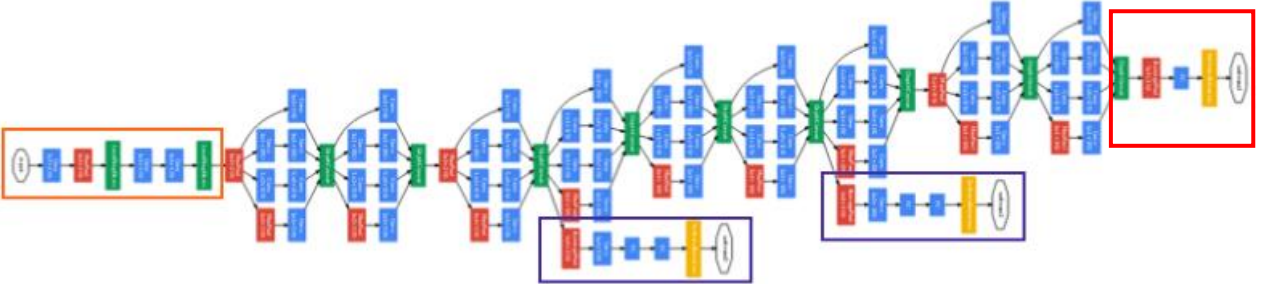
\includegraphics[width=0.7\textwidth]{images/incgoogle.PNG}\par
\end{center}
They introduced 2 extra classifiers. By introducing those classifiers, the loss to be minimized is no more the loss of the final network output but it's the sum of those losses and the final result is taken from that. This is just a trick for the vanishing gradient problem. 

\subsection{ResNet}
This model achieved 3\% performance the following year. There is a completely change of perspective in this network (which today has different versions). For the Inception the purpose was to handle feature patterns of multiple resolutions combining and replicating different sized filters; here the purpose was to design a network that was incredibly deep stacking more and more layers. They find out this:
\begin{center}
    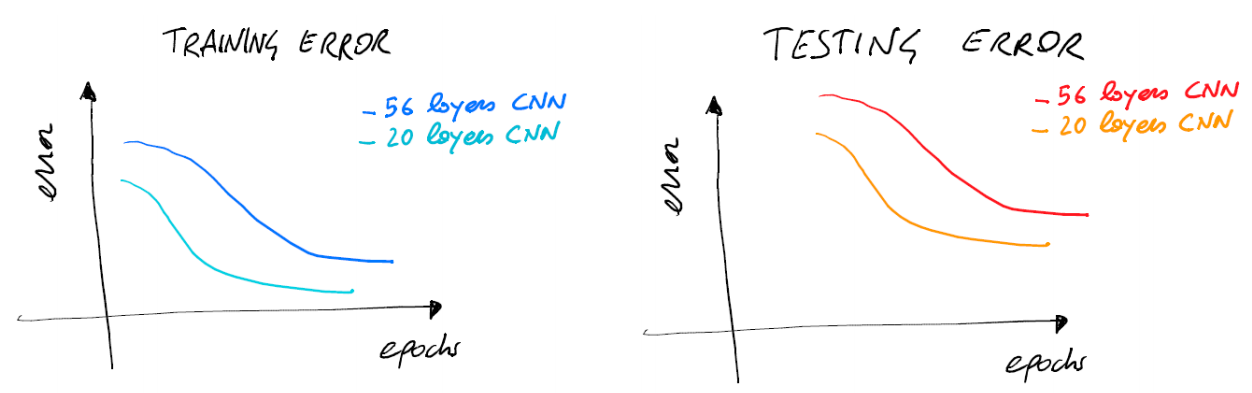
\includegraphics[width=0.9\textwidth]{images/resnet_error.PNG}\par
\end{center}
The testing error for a network with 20 layers and 56 layers had the same trend, but the one with 56 layers was larger. One can think that this is due to overfitting, but this is not the case because training and testing error should diverge but in this case this does not happen. Probably the reason is that you cannot explain the result as an overfitting problem, is just a problem of minimizing the loss function: training deeper networks is harder with respect to shallow networks. They added a skip connection, which corresponds to the identity, copying the parameters of the shallow network into the deeper network; if you are not good at learning deeper networks at least skip connections provide the identity. What happens is that you take the input of the two convolutional layers, which are the weights and non linearities, and what you do is summing the input to the output:
\begin{center}
    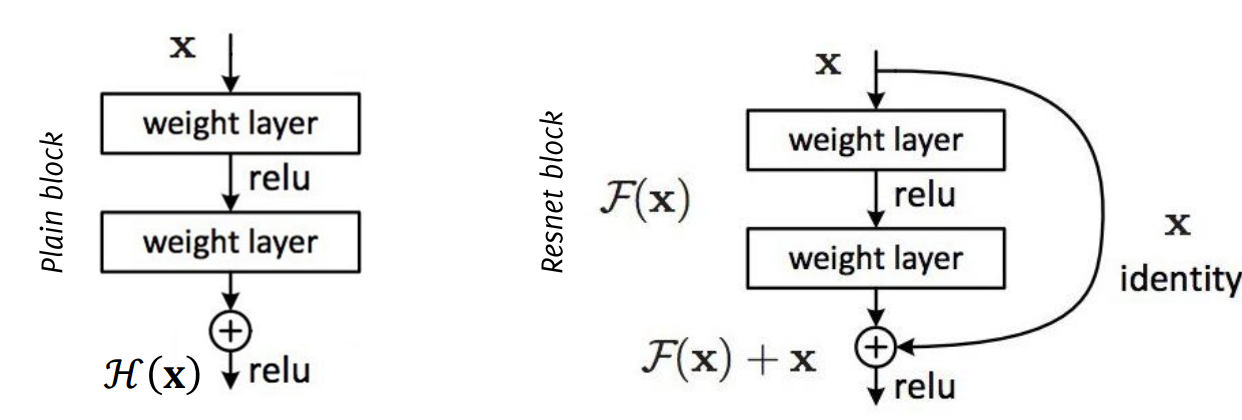
\includegraphics[width=0.6\textwidth]{images/resnet_skip.PNG}\par
\end{center}
This is something easier to train and the substantial increase in performance confirms that skip connections were a good idea. This is called \textbf{\textit{residual network}} because 
%if the ideal function that you would like to learn from a traditional architecture which is the same weights but without the skip connections,
if $H(x)$ is the function that you would like to learn than instead of learning $H(x)$ what you're learning is something like $\mathcal{F}(\mathbf{x})=\mathcal{H}(\mathbf{x})-\mathbf{x}$. Note that this does not add parameters to the network, it's just a copy and a sum, you are just letting the network solve a different learning problem. The weights in between the skip connections can be used to learn a "delta", a residual, $F(x)$ in order to improve the solution achieved by the shallow network.  There are a few consideration, in particular you have to be sure that the spatial extent is the same to perform the sum, so you have to do some padding to adjust the spatial extent. 

The substantial improvement achieved by the ResNet from the Inception (almost 50\% better in the classification error) probably can be justified that deeper networks are able to achieve lower errors, as expected. 

\subsection{DenseNet}
In this architecture there are skip connections everywhere. There are multiple blocks and inside each block the output is connected to each of the previous input for skip connections.

\subsection{Comparison}
You can see a model comparison using as variables the size of the parameters and the performance achieved. The AlexNet was the first actually and it was below 55\%, VGG had a lot of parameters and better performance but not incredibly good. 
\begin{center}
    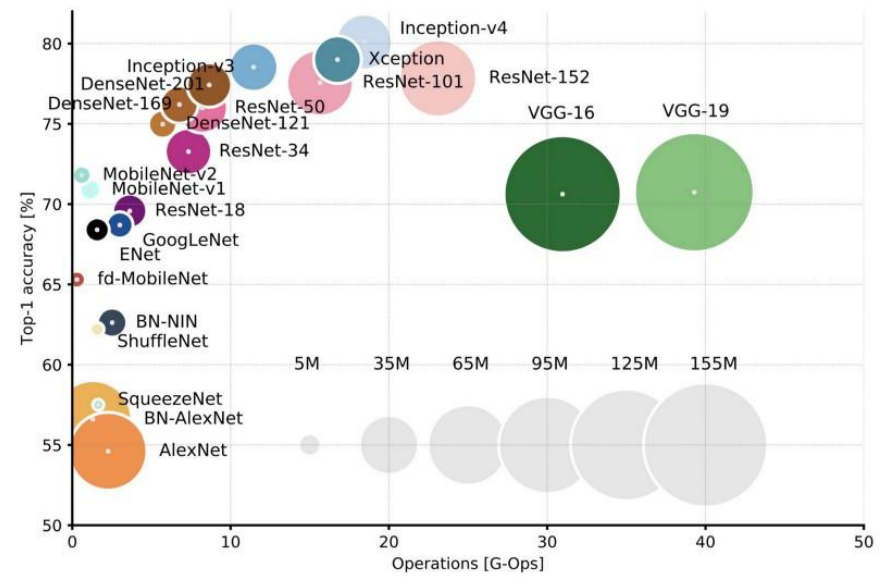
\includegraphics[width=0.75\textwidth]{images/model_comparison.PNG}\par
\end{center}
DenseNet and Inception are quite reduced but achieve very good performance. Inception models are the better performing, in particular the InceptionV4 that combines Inception and ResNet. Another important architecture is MobileNet which has very few parameters and it's very efficient but achieves decent performance; this uses separable convolutions and it's been designed for mobile purposes. 
\section{Generative Adversarial Networks}
This is an hyped field, but first we need some background regarding autoencoders.

\subsection{Autoencoder}
An \textbf{autoencoder} is a network which is meant to learn a sort of identity mapping; you are given an input of input neurons and you train a network which has as output some output neurons and the output is meant to be exactly the same input. The first part that goes from the input to the bottleneck is called \textbf{encoder}, while in output you have the \textbf{decoder}.  
\begin{center}
    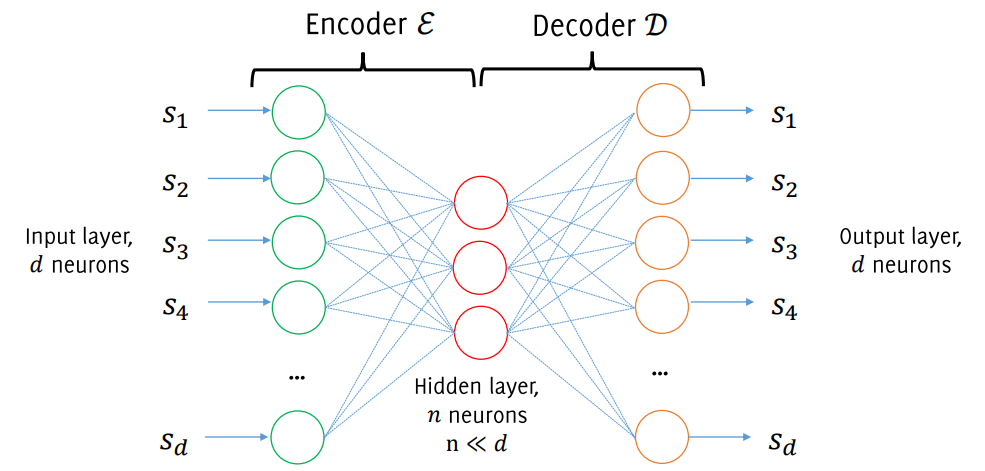
\includegraphics[width=0.75\textwidth]{images/autoencoder.PNG}\par
\end{center}
This seems some stupid task because you are already given the input and you are trying to learn a neural network to transform the input into itself. The autoencoders are used, for example, for data reconstruction. An autoencoder is a type of artificial neural network used to learn efficient data codings in an unsupervised manner. The aim of an autoencoder is to learn a representation (encoding) for a set of data, typically for dimensionality reduction, by training the network to ignore signal “noise”. Indeed, you can design your network to have a bottleneck of much fewer neurons than the input, so you learn a function that compresses our input signal to a lower dimension representation, it's a more compact representation of the input signal. \\
So Autoencoders are non-parametric models that can be trained to reconstruct all the data in a training set. The reconstruction loss is:
\begin{center}
    $\sum_{s \in S}\|s-\mathcal{D}(\mathcal{E}(s))\|_{2}$
\end{center}
The training of $\mathcal{D}(\mathcal{E}(\cdot))$ is done via standard backpropagation algorithms. This is important in the context of having a latent representation of object; with autoencoders you want to learn a \textit{latent representation} which is meant to provide a compact representation of your input which allows to recover the signal (it's like setting a 1-to-1 correspondence).

You can use these autoencoders also in CNN., for example segmentation networks are similar to the architecture of autoencoders. You can train convolutional autoencoders to find some compressed representation removing the noise. \\

Remarks:
\begin{itemize}
    \item[--] Features $z$ are typically referred to as \textbf{latent representation}
    \item[--] Autoencoders typically do not provide exact reconstruction since $n << d$, by doing so we expect the latent representation to be a meaningful and compact representation of the input
    \item[--] Additional \textit{regularization terms} might be included in the loss function
    \item[--] More powerful and non-linear representation can be learned by \textit{stacking multiple hidden layers} (deep architectures)
\end{itemize}{}

These are also useful to perform in practice to provide a \textbf{good initialization} to a network. As soon as you are given a huge amount of train images which are sort of unlabeled (imagine a semi-supervise setting), a way to learn also from not annotated images is the following:
\begin{enumerate}
    \item first you train, using not annotated images, an autoencoder which tries to reconstruct your input, in a fully unsupervised way;
    \item once you have trained the autoencoder, you get rid of the decoder and you keep the compressed representation;
    \item than if you are given some training samples, you plug in the rest of your network for classification purposes and you fine-tune the full network on the training samples. 
\end{enumerate}
In this case you are also able to exploit an unsupervised problem to provide a good initialization and prevent the risk of overfitting. The feature that you learn for reconstruction may not be too good for classification but in principle the first they should be good for the first convolutional features.\\

Autoencoders provide a \textit{good initialization} (and reduce the risk of overfitting) because their latent vector is actually a good representation of the inputs used for training. 

\subsection{Generative Models: Variational Autoencoders}
\textbf{Goal} Generative models generate, given a training set of images (data) $S$, other images (data) that are similar to those in $S$. \\

Generative models can be used for \textit{data augmentation}, simulation and planning. \\
Training generative models can also enable inference of latent representation that can be useful as general features. \\

What about using Autoencoders as Generative Models? \\
The important thing for us in this case is the latent representation that we get from an autoencoder. This latent representation is good at describing images but wouldn't be good at generating images. Given an image I can compress and decompress it, so one option could be to take the decoder network $\mathcal{D}$ and discard the encoder. Variational autoencoders leverage a prior distribution learnt by the autoencoders over $z$ to generate images with an architecture similar to this. \\
The procedure: 
\begin{enumerate}
    \item Train an autoencoder on $S$
    \item Discard the encoder
    \item Draw random vectors to replace the latent representation and feed this to the decoder input
\end{enumerate}
\begin{center}
    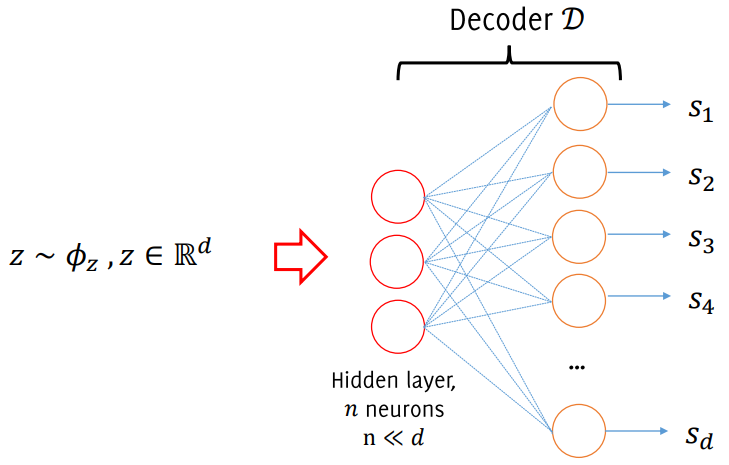
\includegraphics[width=0.6\textwidth]{images/autogenerative.PNG}\par
\end{center}
Unfortunately this does not work, you cannot randomly generate an image by just throwing some random numbers inside the latent representation. The problem is that we don't know the distribution of proper latent representation (or it's very difficult to estimate it). The goal is to find out a way to randomly generate images that actually look like a real image, an image with a meaning. This task was solved by \textbf{Generative Adversarial Networks}.

\subsection{Generative Models: GANs}
We are not looking for an explicit density model $\phi_{s}$ describing the "secret" manifold of natural images, we just want to find out a model able to generate samples that look like training samples.

Instead of sampling from $\phi_{s}$, just:
\begin{itemize}
    \item[--] Sample a seed from a known distribution $\phi_{z}$
    \item[--] Feed this seed to a learned transformation that generates realistic samples, as if they were drawn from $\phi_{s}$
\end{itemize}{}
We will be given some sort of random distribution $\phi_{z}$ which is a uniform distribution over a $d$-dimensional space. From the distribution we sample a seed $z$, which is a random number with $d$ components and $\phi_z$ is the distribution used to generate this number.\\
Now what I would like to do is to train a network $\mathcal{G}$ that takes as input $z \sim \phi_{z}, z \in \mathbb{R}^{d}$ and provides me $\mathcal{S}$ which is a "nice" image and of course belongs to $\mathbb{R}^{n}$, in particular it belongs to the secret manifold of images. In general what I want is taking a random noise, feed it to a generative network and obtain an image like this that's randomly generated:
\begin{center}
    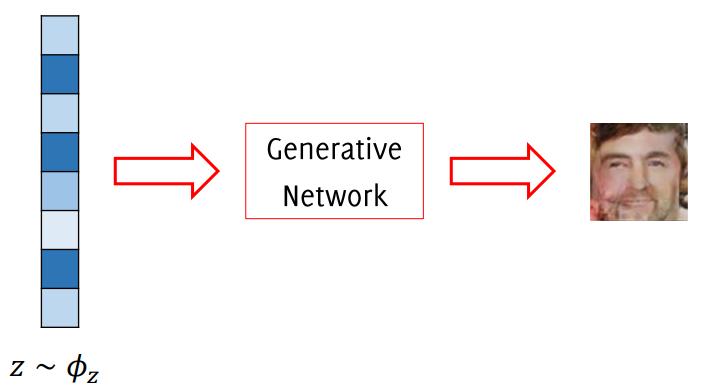
\includegraphics[width=0.6\textwidth]{images/gan_vecchio.PNG}\par
\end{center}
If you change the noise, you get a different image. 

Why is this problem challenging?\\
What misses here is an \textit{appropriate loss function}. The loss function should tell how "happy" we are with the output image, and being happy means that the image looks like a natural image. Obviously this is hard to measure because you need a number, so the trick of GANs was to replace this loss with another neural network, called \textbf{discriminator} $\mathcal{D}$.\\
The discriminator network $\mathcal{D}$ is trained to determine if the images generated by the generator network $\mathcal{G}$ are real, to classify between real and fake images. 

Thus, The GAN solution is to train a pair of neural networks with different tasks that compete in a sort of two player game.\\
The models are:
\begin{itemize}
    \item \textbf{Generator} $\mathcal{G}$ that produces realistic samples e.g. taking as input some random noise. $\mathcal{G}$ tries to fool the discriminator
    
    \item \textbf{Discriminator} $\mathcal{D}$ that takes as input an image and assess whether it is real or generated by $\mathcal{G}$
\end{itemize}{}
Train the two model and at the end, keep only $\mathcal{G}$ \\

The key idea is that instead of having a measure of how much our image looks like a natural image, you train another network simultaneously which in this context operates like a loss function. After a successful GAN training, the discriminator $\mathcal{D}$ is completely useless because it is no longer able to distinguish between real and fake images and the generator is able to cheat the discriminator, so we throw it away and we take only the generator $\mathcal{G}$.

Let's write this formally. Let's call $\mathcal{G}$ the generator and $\mathcal{D}$ the discriminator.
\begin{center}
    $\mathcal{D}=\mathcal{D}\left(\boldsymbol{s}, \theta_{d}\right)$ \\
    $\mathcal{G}=\mathcal{G}\left(\mathbf{z}, \theta_{g}\right)$
\end{center}
(\textbf{Note} that the role of n and d are reversed: from now on, n is the size of an image and d is the size of the input noise)\\
 These networks will have some parameters $\theta_{d}$ and $ \theta_{g}$, $\boldsymbol{s}\in \mathbb{R}^{n}$ is an input image (either real or generated by $\mathcal{G}$) and $\boldsymbol{z}\in \mathbb{R}^{d}$ is some random noise to be fed to the generator network. 
 Our network gives as output:
\begin{itemize}
    \item[--] The posteriori for an input to be a true image: $
\mathcal{D}\left(\cdot, \theta_{d}\right): \mathbb{R}^{n} \rightarrow[0,1]
$
    \item[--] The generated image: $
\mathcal{G}\left(\cdot, \theta_{g}\right): \mathbb{R}^{d} \rightarrow  \mathbb{R}^{n}
$
\end{itemize}{}
A good discriminator is such: 
\begin{itemize}
    \item $\mathcal{D}\left(\boldsymbol{s}, \theta_{d}\right)$ is maximum when $s \in S$
    \item $ 1 - \mathcal{D}\left(\boldsymbol{s}, \theta_{d}\right)$ is maximum when $s$ was generated from $\mathcal{G}$
    \item $ 1 - \mathcal{D}\left(\mathcal{G}\left(\boldsymbol{z}, \theta_{g}\right), \theta_{d}\right)$ is maximum when $\boldsymbol{z} \sim \phi_z $
\end{itemize}{}
 When training $\mathcal{D}$ we try to maximize the binary cross-entropy, the classification accuracy, so training $\mathcal{D}$ means solving this classification problem:
 \begin{center}
     $\max _{\theta_{d}}\left(\mathrm{E}_{s \sim \phi_{S}}\left[\log \mathcal{D}\left(\boldsymbol{s}, \theta_{d}\right)\right]+\mathrm{E}_{z \sim \phi_{Z}}\left[\log \left(1-\mathcal{D}\left(G\left(\mathbf{z}, \theta_{g}\right), \theta_{d}\right)\right)\right]\right)$
 \end{center}
$\mathrm{E}_{s \sim \phi_{S}}$ is the expectation, which is replaced in practice by an average over mini-batch, of $S$ drawn from $\phi_{S}$ (the distribution of natural images),  so this is the expectation over the distribution of natural images. When images are drawn from the manifold you want the first probability part to be large, while you want the probability to be small when images are drawn from the fake distribution (when they are generated by $\mathcal{G}$). The first term is the probability that the discriminator gives to an image that is true, so you want this to as close as possible to 1:
\begin{itemize}
    \item $\mathrm{E}_{s \sim \phi_{S}} [\log \mathcal{D}\left(\boldsymbol{s}, \theta_{d}\right)] $ has to be 1 since $s \sim \phi_S$, thus images are real
\end{itemize}{}
$\mathrm{E}_{z \sim \phi_{Z}}$ is the expectation over the fake distribution generated by the generator network. The second term is the probability that you want to be zero because that image is not a natural image. 
\begin{itemize}
    \item $\mathrm{E}_{z \sim \phi_{Z}} [\log ( 1 -  \mathcal{D}\left(\mathcal{G} (\boldsymbol{z}, \phi_g), \theta_{d}\right)] $ has to be 0 since $\mathcal{G} (\boldsymbol{z}, \phi_g)$ is a generated (fake) image
\end{itemize}{}
You train the neural network to maximize this sum which is the sum of the probabilities for real images and one minus the probability of fake images. \\

Now let's move to $\mathcal{G}$: a good generator $\mathcal{G}$ is the one which makes $\mathcal{D}$ \textbf{to fail}. \\
A good loss for $\mathcal{G}$ would be something that tells that the discriminator fails because we are trying to trick the discriminator providing fake images that seem real, it's a two player game. We'd like to find the parameter $\theta_{g}$ in order to minimize this:
\begin{center}
    $\min _{\theta_{g}} \max _{\theta_{d}}\left(\mathrm{E}_{S \sim \phi_{S}}\left[\log \mathcal{D}\left(\mathbf{s}, \theta_{d}\right)\right]+\mathrm{E}_{z \sim \phi_{Z}}\left[\log \left(1-\mathcal{D}\left(G\left(\mathbf{z}, \theta_{g}\right), \theta_{d}\right)\right)\right]\right)$
\end{center}
The generator should minimize the effectiveness of the discriminator. It's a min-max optimization, you have to perform the optimization simultaneously but typically it is difficult to solve directly, so what you do in practice is alternate: 
\begin{enumerate}
    \item First you do $k$-steps of SGA (in this case you perform the ascent gradient obviously) maximizing the discriminator function taking $\mathcal{G}$ fixed and optimize for $\mathcal{D}$
    $$ \max _{\theta_{d}}\left(\mathrm{E}_{S \sim \phi_{S}}\left[\log \mathcal{D}\left(\mathbf{s}, \theta_{d}\right)\right]+\mathrm{E}_{z \sim \phi_{Z}}\left[\log \left(1-\mathcal{D}\left(G\left(\mathbf{z}, \theta_{g}\right), \theta_{d}\right)\right)\right]\right)$$
    
    \item Then  you take $1$-step of SGD  maximizing the generator function taking $\mathcal{D}$ fixed and optimize for $\mathcal{G}$
    $$ \min _{\theta_{g}}\left(\mathrm{E}_{S \sim \phi_{S}}\left[\log \mathcal{D}\left(\mathbf{s}, \theta_{d}\right)\right]+\mathrm{E}_{z \sim \phi_{Z}}\left[\log \left(1-\mathcal{D}\left(G\left(\mathbf{z}, \theta_{g}\right), \theta_{d}\right)\right)\right]\right)$$
    
    we can remove the first term because it does not depend on $\theta_g$:
    $$ \min _{\theta_{g}}\left(\mathrm{E}_{z \sim \phi_{Z}}\left[\log \left(1-\mathcal{D}\left(G\left(\mathbf{z}, \theta_{g}\right), \theta_{d}\right)\right)\right]\right)$$
    
    Nothing changes if we use Gradient Ascent instead of Gradient Descent unless for the change from $min$ to $max$: 
    $$ \min _{\theta_{g}}\left(\mathrm{E}_{z \sim \phi_{Z}}\left[\log \left(1-\mathcal{D}\left(G\left(\mathbf{z}, \theta_{g}\right), \theta_{d}\right)\right)\right]\right) \longrightarrow \max _{\theta_{g}}\left(\mathrm{E}_{z \sim \phi_{Z}}\left[\log \left(\mathcal{D}\left(G\left(\mathbf{z}, \theta_{g}\right), \theta_{d}\right)\right)\right]\right)$$
    
    This change does not modify the global solution of the min-max problem, but provides a stronger gradient during the early learning stages.
\end{enumerate}
%first you do $k$-steps of SGA (in this case you perform the ascent gradient obviously) maximizing the discriminator function and then you take $1$-step of SGD  maximizing the generator function, so you leave $\mathcal{G}$ fixed and optimize for $\mathcal{D}$ and then you leave $\mathcal{D}$ fixed and optimize for $\mathcal{G}$. Once $\mathcal{D}$ is fixed after $k$-steps you only have to minimize, this means that you can have one step of SGD, and you alternate between the two.\\
Moreover, in order to achieve convergence, instead of  $\min \nabla_{\theta_{g}}\left[\sum_{i} \log \left(1-\mathcal{D}\left(\mathcal{G}\left(\mathbf{z}_{i}, \theta_{g}\right), \theta_{d}\right)\right)\right]$, it's better to  %minimize
$\max \nabla_{\theta_{g}}\left[\sum_{i} \log \left(\mathcal{D}\left(\mathcal{G}\left(\mathbf{z}_{i}, \theta_{g}\right), \theta_{d}\right)\right)\right]$.

Summing up, for $k$ times you draw a minibatch of noise realizations $z$, you sample a minibatch of images and then you update $\mathcal{D}$ by SDA; then you draw a minibatch only of noise realizations and you just update $\mathcal{G}$ by SDG, which in practice is SGA for what we just said about convergence. \\

\begin{minipage}{\linewidth}
\centering
\hspace*{-2cm}    
\begin{minipage}{9cm}
  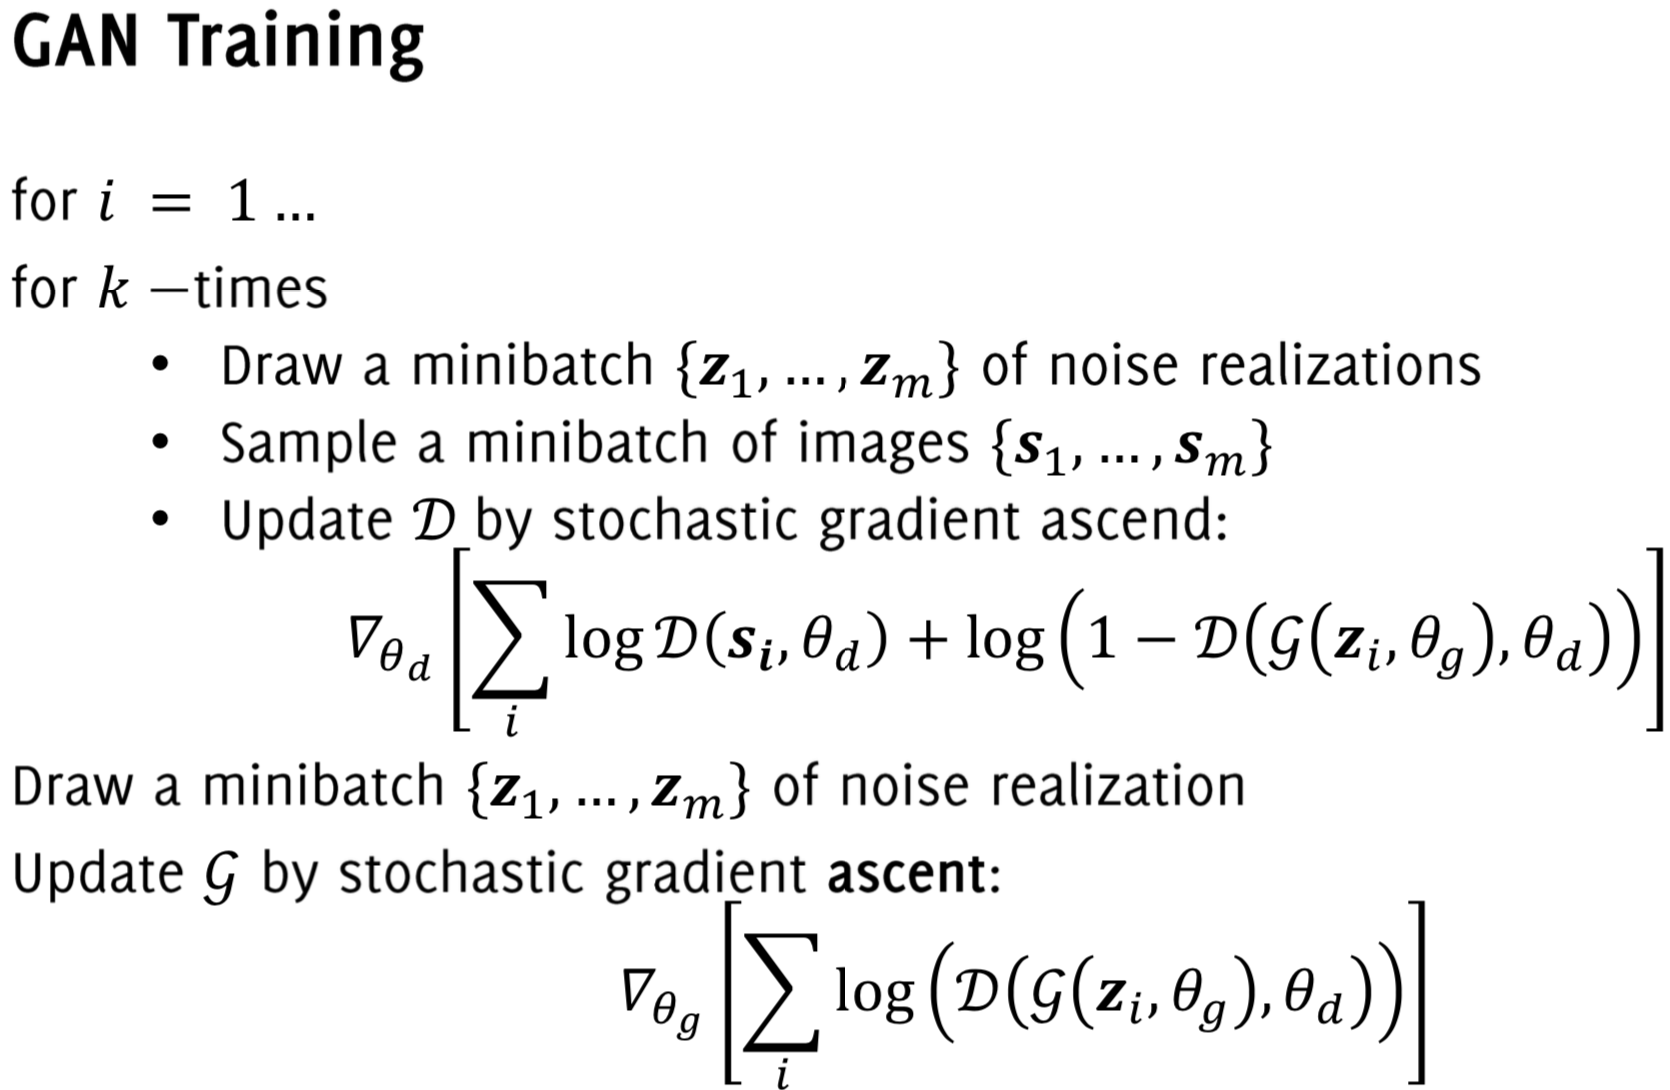
\includegraphics[width=9cm, height=7cm]{images/gan_sgd.png}
  %\captionof{figure}{A figure}
  %\label{fig:test1}
\end{minipage}%
\begin{minipage}{10cm}
  \centering
  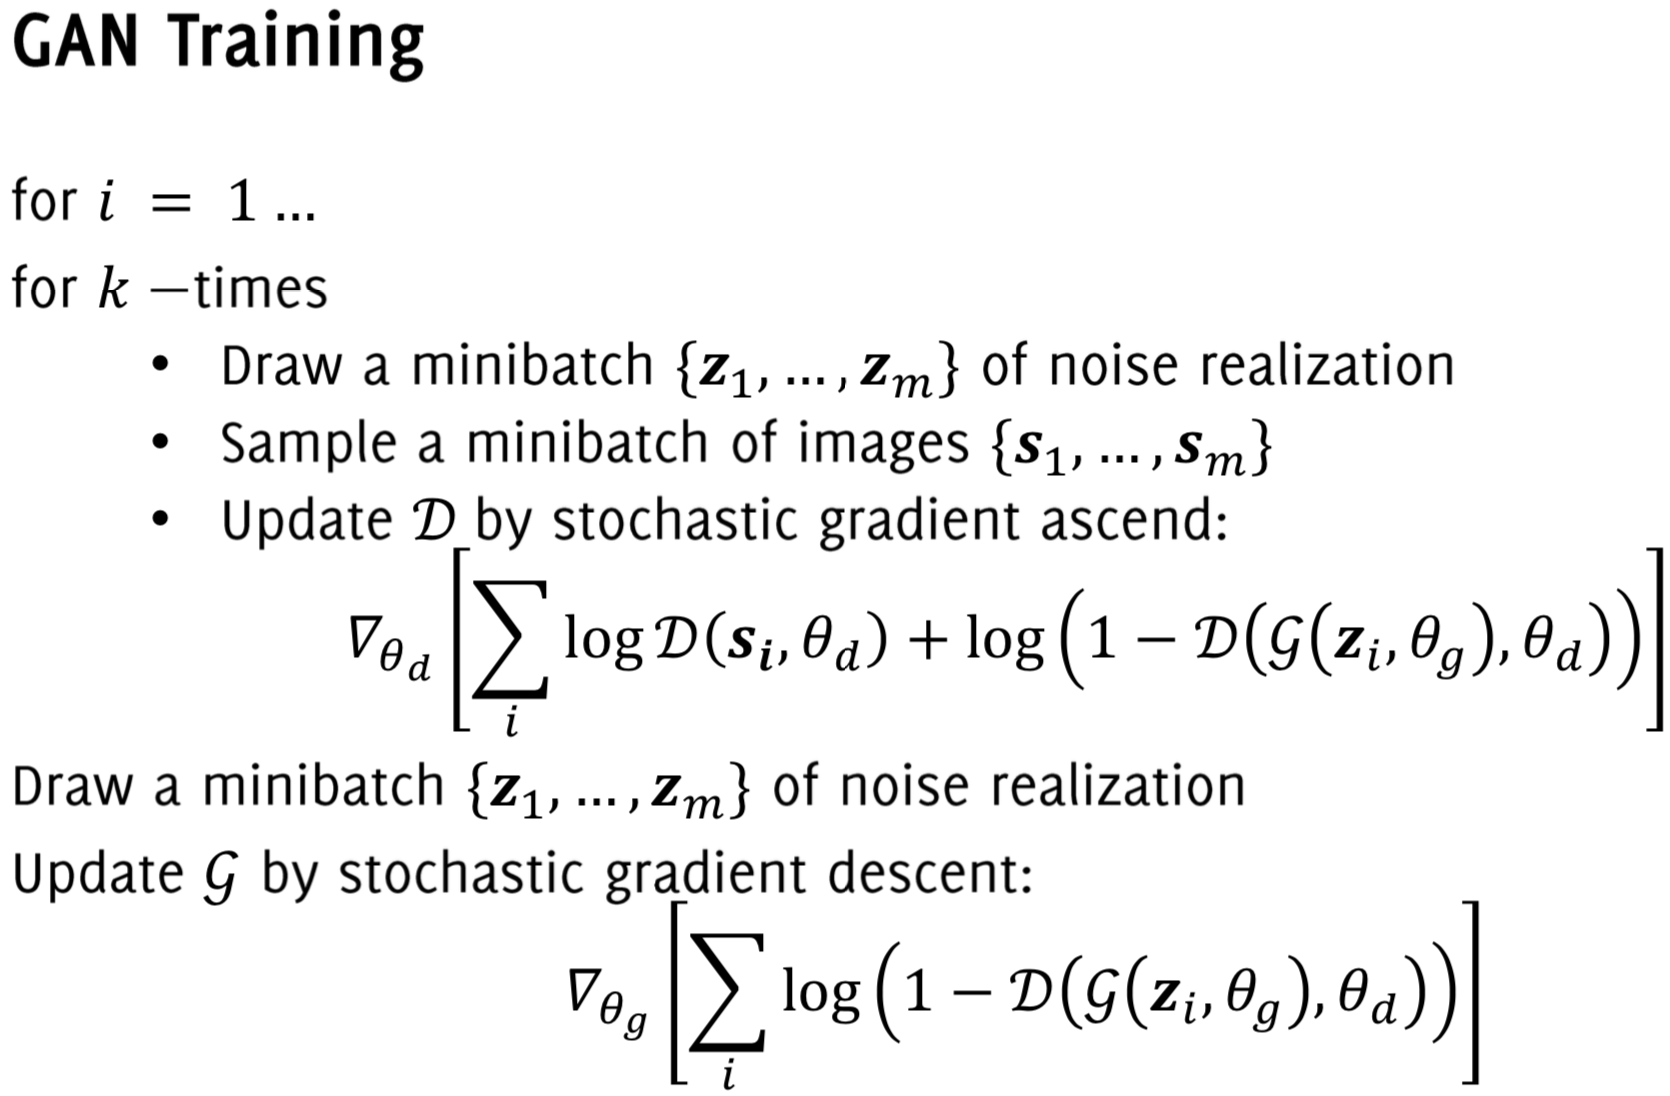
\includegraphics[width=9cm, height=7cm]{images/gan_sga.png}
  %\captionof{figure}{Another figure}
  %\label{fig:test2}
\end{minipage}
\end{minipage}\\ \\

This illustration shows how the training proceeds:
\begin{center}
    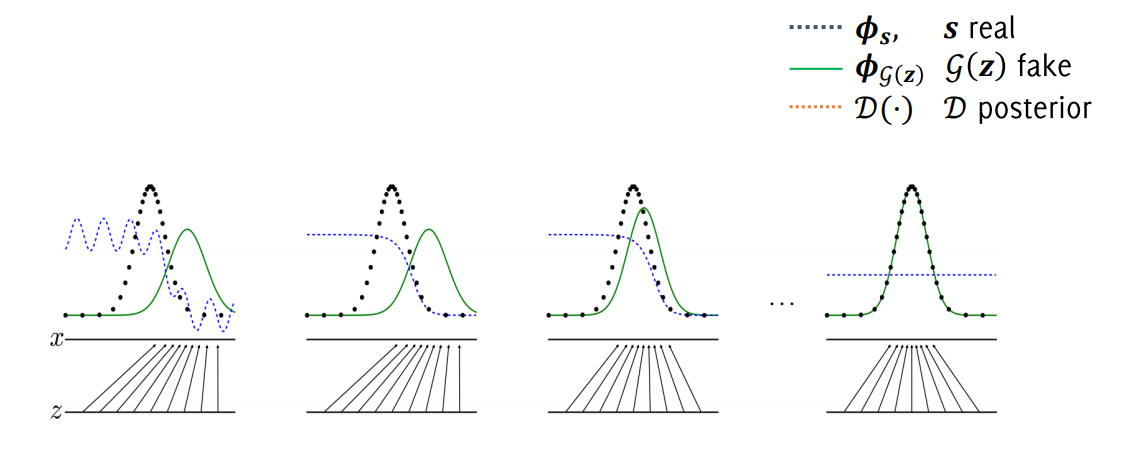
\includegraphics[width=0.8\textwidth]{images/gan_training.PNG}\par
\end{center}
Again $\phi_{s}$ is the real manifold where natural images live, it's what you want to be able to sample, and $\phi_{z}$ is the distribution of noise which are feed to the generator to get an image. At the very beginning, the images that you generate are very far from the natural images. When training better $\mathcal{D}$ you are defining better the separation between the two classes, the one generated by the network and the one of real images; but now when you are training $\mathcal{G}$, what you do is steering your generator network to provide images that are more realistic and closer to the distribution of real images. As the training proceeds, the two distribution finally overlap and the discriminator gives 0.5 probability (random probability) because it can no longer distinguish between real and fake. This is \textbf{unstable to train} but it's trained by standard tools: backpropagation and dropout. What is important is that the generator does not use directly $\mathcal{S}$ for training, it just takes as input random noise and the real images are just used in order to define some sort of loss through the game with the discriminator.\\
Generator performance is difficult to assess quantitatively. There is \textbf{no explicit} expression for the generator, it is provided in an \textbf{implicit} form $\rightarrow$ you cannot compute the likelihood of a sample w.r.t. the learned GAN
\section{Recurrent Neural Networks}
So far we have considered only \textit{static} datasets: input and output don't have any time, any ordering or dependencies between each other.\\
(Aggiungere figura sequencernn)\\
The main idea is to think the input as a vector $X_i$ and consider a sequence of inputs in order to model that sequence of samples. 

Some relevant sequence are, for instance, time-series or text that, in general, are some sort of \textit{dynamical} data. To model this sequence you have different approaches: 
%So far input and output don't have time, do not have any ordering or dependences between each other.

%slide 3
%The idea is to think about the input as a vector and you have a sequence of input. We would like to go beyond the idea of having input and output and the model we are building is independent from the sequence of the samples , acutally we want to model the sequence of the samples. Some sequence relevant are time-series but also text. The idea is that we have a sequence of input and we would like to model this sequence. To model this sequence, you have different approach: 

\begin{itemize}
    \item \textbf{Memoryless} models: you don't explictly store a representation of the past, but you just use the previous $k$-samples to predict the next one
        \begin{itemize}
            \item  \textit{Autoregressive models}: predict the next input from previous ones using "delay taps"
            \item \textit{Feed Forward Neural Networks}: generalize autoregressive models using non-linear hidden layers. You feed your network with the $k$ past samples and you try to predict the next one. This approach is known as \textit{Sliding Window}        \end{itemize}{}
    \item \textbf{Memory-based} models: they are generative models with a real-valued hidden state which cannot be observed directly. The hidden state has some dynamics possibly affected by noise and produces the output. To compute the output the model has to infer hidden state. Input as treated as driving inputs.
        \begin{itemize}
            \item  \textit{Linear Dynamical System}: keep the state of the system which models the evolution of your data and define an output function which models the output given the current state of the system. In Linear Dynamical Systems the system becomes state continuous with Gaussian uncertaintly, transformations are assumed to be linear and the state can be estimated using \textit{Kalman Filtering}. One observation is that if you model your data in this way, you get a \textbf{stochastic} system. 
            \item \textit{Hidden Markov models}: you have a random variable which models the state of the system and another one that models the output of the system. The state is assumed to be discrete, state transitions are \textit{stochastic} (transition matrix). The output is a \textit{stochastic} function of hidden states. The states can be estimated via \textit{Viterbi algorithm}. In this model you do not have any input, but only a hidden state. This is a \textbf{stochastic} system
            \item  \textit{Recurrent Neural Network}: they are \textbf{deterministic} systems and they will be deepened more in the following chapters. 
        \end{itemize}{}
\end{itemize}{} 



%A model that is memory-less, you don't explicitly store a representation of the past but you just use the previous k-samples to predict the next one. This can be done with auto-regressive model or via feed-forward neural network. 

%(immagine appunti) To use a FNN to predict the next sample basing on the last two, you fed your network with the two inputs of the previous steps. You treat these two sample as input and you try to predict the next one. You don't need memory: this approach is know as Sliding Window. You don't necessary need memory to model time series. 

%You have also models with memory:
%Linear Dynamical systems: where you have a state of the system which model the evolution of your data and an output function which models the output given the current state of the system 

%Hidden Markov Model: evolution of the previous. You have a random variable which model the state of the system and another which models the output of the system

%Recurrent Neural Network: verranno approfondite

%slide 5 
%So in auto regressive model: you have a sequence of states, if the blocks represents the state or the output of the system at time zero, you try to predict one state looking k-step before.
%With FNN you generalize the classical linear model by having an hidden state. In this case, X2 is a function of x1 and x0 through an hidden state.

%slide 6
%If you want to do a change you have to add a state. For instance, you can have a model like this where your current input modify a state, your state impacts on the output. At the next time, the previous state is put forwarded, it is modified with the current input and generate the output, and so on and so forth, the state is put forward and so. The memory is hidden in the model and it is put forward while you do prediction.
%The idea is that you have some dynamics in the state and basically to compute the output you have to detect or estimate what is the current value of the state. If you have continuous state and linear transformation, it is basically linear Gaussian model and inferring the value of the state is what you do with a classical Kalman Filter. 
%One observation is that if you model your data in this way, you get a stochastic system.
%Another approach is the Hidden Markov model where you don't have the input, you have only an hidden state. 
%In neural network the things are more complex. 
%(so google presentation fare un'unica immagine con le varie figure alle slides 5-6-7 e mettere una label di quale modello si riferiscono)

\subsection{Recurrent Neural Networks}
Let's start modeling a standard system with a standard Feedforward Neural Network such as the one seen so far: the output is a non linear function of the weighted sum of the hidden neurons and these hidden neurons are a non linear function of the weighted sum of the input. \\ 
The classical way to add the memory is through \textit{Recurrent Hidden Neurons}, the blue ones in the Fig.\ref{wrap-fig:rnn}: a set of hidden neurons is added and their outputs are recurred. These hidden neurons have a feedback loop which makes their output depending on the previous value. \\
Memory via recurrent connections has some benefits:
\begin{itemize}
    \item Distributed hidden state allows to store a information efficiently
    \item Non-linear dynamics allows complex hidden state updates
\end{itemize}{}

\begin{wrapfigure}{l}{8.5cm}
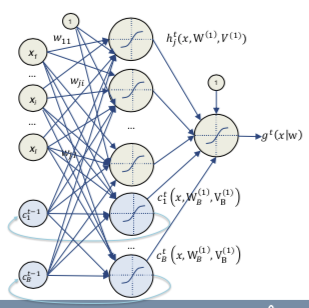
\includegraphics[width=8.5cm, height=7.2cm]{images/rnn.png}
\caption{Recurrent Neural Network}\label{wrap-fig:rnn}
\end{wrapfigure} 
 
These approach is due to Helmann and it is different from linear dynamical systems since one part of the hidden layer [the brown part] is \textit{time-less} and the other part is in charge of bringing forward the information. The blue part is a sort of summary of all the input that the network have seen so far. This summary is brought forward to the next step and it becomes non-linear combination of the previous state and the current input. \\
The blue nodes are also called \textit{c-nodes} because they provide the context to create the output.\\ \\
The context part of the network depends on the previous value of the context network and the current input which update the state: in fact, the \textit{context-neuron} is : 
%Adding the memory: the classical way the memory is added to a neural network is through recurrent hidden neurons(?). The most common way is to add a set of hidden neurons (the blue ones) and recur their outputs. These hidden neurons have a feedback loop which makes their output depending on the previous value. This is different from the linear dynamical system, since one part of the hidden layer (the brown part) is time-less and the other part (the blue) is in charge of bringing forward the information. You can image the blue part a sort of summary of all the input that the network have seen so far. This summary is brought forward to the next step, and the summary becomes non linear combination of the previous state and the current input. This model is due to Helmann. So you see the output depends also on the c-nodes. The c-nodes provides the context to provide the output. Context network depend on the previous value of the context network and the current input which update the state: in fact, the context-neuron is written as: 
$$
c_{\mathrm{B}}^{\mathrm{t}}\left(x, \mathrm{W}_{\mathrm{B}}^{(1)}, \mathrm{V}_{\mathrm{B}}^{(1)}\right)
$$
where $x$ is the input, $W_B$ are the weights from the input to the context network and $V_B$ are the weights from the context network to itself, so from the previous step to the current step.
In the figure there are other weights from $c_i^{t-1}$ to the brown neurons (from the context to the hidden) that can  be called $V$.\\
In general, the main formula of the RNN are shown below
$$
\begin{aligned}
g^{t}\left(x_{n} | w\right) &=g\left(\sum_{j=0}^{J} w_{1 j}^{(2)} \cdot h_{j}^{t}(\cdot)+\sum_{b=0}^{B} v_{1 b}^{(2)} \cdot c_{b}^{t}(\cdot)\right) \\
h_{j}^{t}(\cdot) &=h_{j}^{t}\left(\sum_{i=0}^{I} w_{j i}^{(1)} \cdot x_{i, n}+\sum_{b=0}^{B} v_{j b}^{(1)} \cdot c_{b}^{t-1}\right) \\
c_{b}^{t}(\cdot) &=c_{b}^{t}\left(\sum_{i=0}^{I} v_{b i}^{(1)} \cdot x_{i, n}+\sum_{b^{\prime}=0}^{B} v_{b b^{\prime}}^{(1)} \cdot c_{b^{\prime}}^{t-1}\right)
\end{aligned}
$$

%(immagine esempio appunti)

\begin{quote}
    \textit{"With enough neurons and time, RNNs can compute anything that can be computed by a computer}
\end{quote}{}

In 1990 there was a theorem that proves that if you have enough neurons and time, you can prove that this model is Turing-complete, as powerful as Turing machine.\\
This recurrent loop needs to be estimate: back-propagation needs that all the function %reverse
to be differentiable and the network to be feed-forward, but this architecture is not feed-forward anymore. So we have to modify back-propagation or find different algorithm to discover this loop. 

%Note: the different between rnn and hidden markov model or linear dynamical system is that, the latters are stochastic, this is deterministic: once you put an input, the output is always the same. It's non linear, complex but deterministic. 
If you want to consider the output at time t:
$$
g^{t}\left(x_{n} | w\right)=g\left(\sum_{j=0}^{l} w_{1 j}^{(2)} \cdot h_{j}^{t}(\cdot)+\sum_{b=0}^{B} v_{1 b}^{(2)} \cdot c_{b}^{t}(\cdot)\right)
$$
it is divided in two part, the forward and the recurrent respectively. We assume $B$ hidden neuron in the context part, $J$ are the neuron in the hidden state. \\
The context network is combination of previous values of the context network and the weighted sum of the input.\\ \\
%You can distinguish between forward and recurrent network. 
Instead, the \textbf{context update} is a non-linear function $c_b^t$ of the weighted sum of the previous context plus the linear combination of the current input. \\
We have more weights but not necessary in form of numbers but as a sort of weights, in the sense that the weights from the previous values of the memory state to the current value of the memory state are tricky to be defined because they represent the memory: these weights are the feedback loop.\\ 

But how to build the context part of the network? \\
%27:50
By definition, the previous %[version]
layer of the hidden state has the same number of  memory states because they are the same thing: basically, you have $B$ hidden neurons here in the context network [we are referring on the blue neurons on the right in Fig.\ref{wrap-fig:rnn}] and $B$ inputs which are the previous values of those hidden neurons, so the number of weights is $B*B$ and this is why you see here
$$
c_{b}^{t}(\cdot)=c_{b}^{t}\left(\sum_{i=0}^{I} v_{b i}^{(1)} \cdot x_{i, n}+\sum_{b^{\prime}=0}^{B} v_{b b^{\prime}}^{(1)} \cdot c_{b^{\prime}}^{t-1}\right)
$$
$b^{'}$ which goes from 0 to $B$ of the weights from $b^{'}$ to $B$.\\
This is a relevant part because we want to learn these weights via back-propagation, but while it's a reasonable standard back-propagation in the brown part, it's more tricky to have back-propagation in the blue part.\\ 

The trick is called \textbf{Back-propagation Through Time} and it is based on the following idea: \\
if the input $V_B^t$ is the output of the previous neuron, I can replicate this structure back in time and I can use the input $V_B^{t-1}$ to the previous neuron. So if the output at time $t$ is $
c_{B}^{t}\left(x, W_{B}^{(t)}, V_{B}^{(t)}\right)
$ , i.e. a combination of its previous value and the current input, I can replicate this node back.
%and now I have an output and I have an input which is the previous step to the (qualcosa). 
So you can back-propagate through these weights. Obviously to get the output you have to back-propagate again and again and again. \\
\begin{figure}
    \centering
    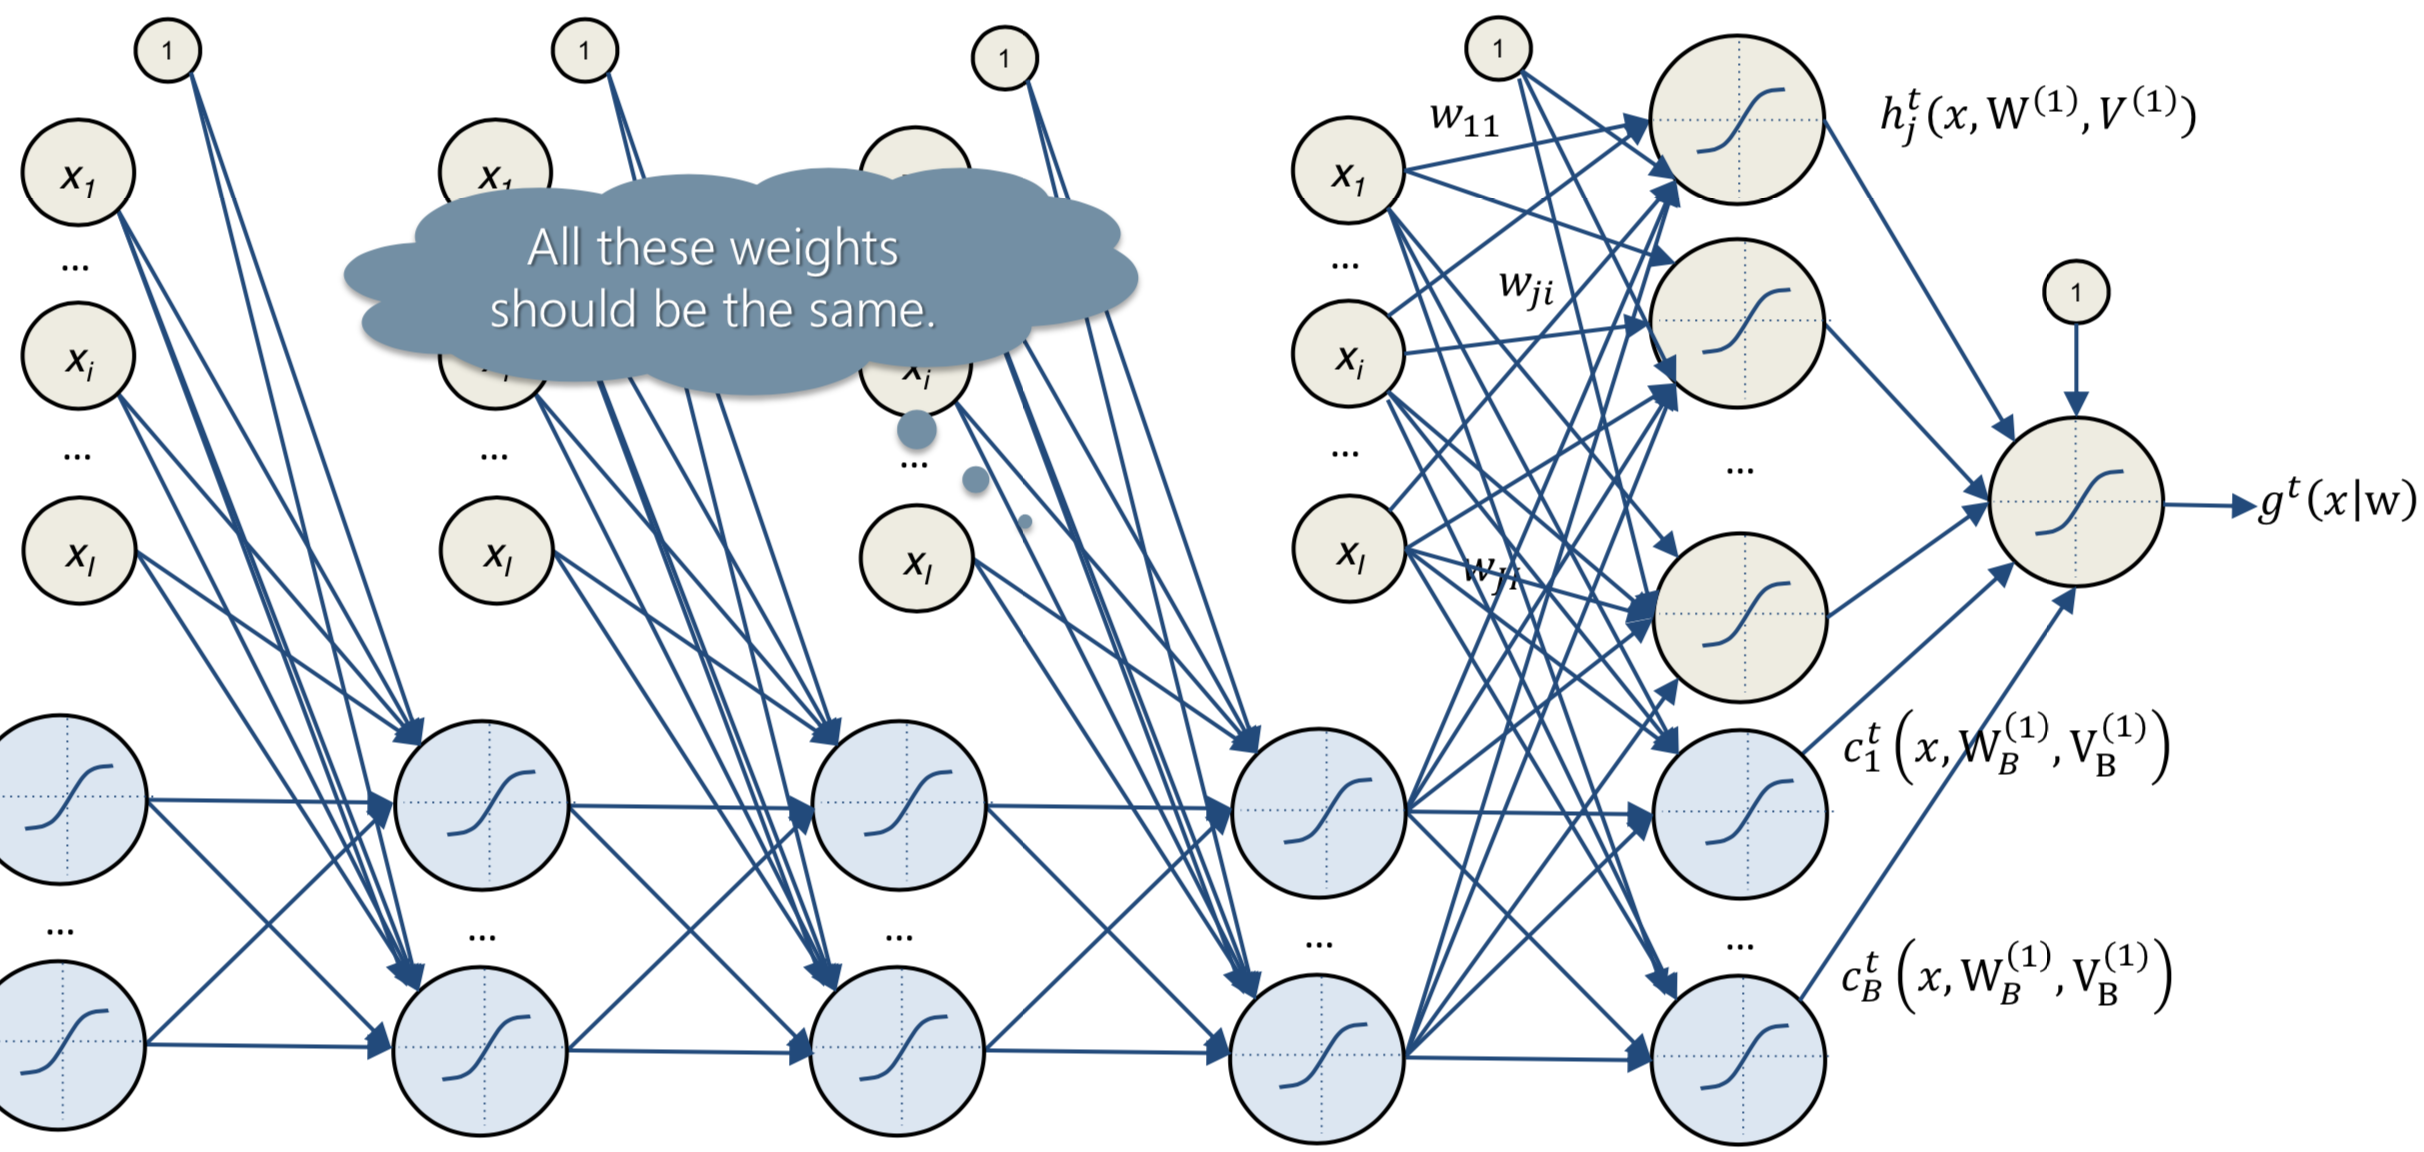
\includegraphics[width=15cm, height=7cm]{images/rnn_backpropagation.png}
    \caption{Backpropagation Through Time}
    \label{fig:rnn_back}
\end{figure}{}

The idea is to make multiple copies of the context network and associate weights to them, so you can back-propagate as a standard Feedforward Neural Network: it's standard because your dataset is finite so you do not need an infinitely long training sequence; if your training sequence has an hundred samples, you unroll for an hundred steps and you can back-propagate on that. \\
The problem is that this approach is not really sustainable for very long sequences, so you have to unroll until a certain point: this approach is called \textbf{Truncated Back-propagation}. This may look like limiting because you do not show, to the network, sequences longer than the limit imposed, but in practice it is not a limitation. \\ 
%Unrolling for 10 or 100 steps does not improve the performance of the model. 
One approach instead of doing full back-propagation can be to slice your dataset in chunks and unroll for the length of the chunks. So the idea is that you start from your loop and you unroll, then you get in principle a feedforward neural network. \\ 

%slide 11
Another important observation is that all the weights of the unrolled part must be the same through all the layers because if you run back-propagation in one neuron (such as the most right blue one), the gradient will be "the error x the derivatives x these weights x derivatives x the output of this neuron"; instead the gradient on the most left neuron %(credo)
is "derivative of the error x derivative of this x weights x derivative x weights x ... and so on (starting from the right to the left) x the output of this neuron". The two gradients %derivatives (forse intendeva i gradient?) 
are different because are computed via different formula. \\
The point is that if you unroll and you treat this "fake" feedforward neural network as classic feedforward neural network, you will end up with an inconsistency because all the weights should be equals %(non so di quali stia parlando)
$\rightarrow$ you have to implement back-propagation by forcing all these replicas to have the same value.\\
In practice, instead, works as follows:
\begin{itemize}
    \item Perform network unroll for $U$ steps
    \item Initialize $V,V_B$ matrices (all the replicas) to be the same. The trick is here, to keep them equal, initialize them equal.
    \item Compute gradients, but you update using the average gradient of all the copies, so you update replicas with the average of their gradients
    $$
    V=V-\eta \cdot \frac{1}{U} \sum_{0}^{U-1} \frac{\partial E}{\partial V^{t-u}}  \quad V_{B}=V_{B}-\eta \cdot \frac{1}{U} \sum_{0}^{U-1} \frac{\partial E}{\partial V_{B}^{t-u}}
    $$
\end{itemize}
There are two ways to perform this pipeline:
\begin{enumerate}
    \item Unroll $\rightarrow$ Compute Gradient  $\rightarrow$ Update all the weights independently  $\rightarrow$ Compute the Average Gradient
    \item Unroll  $\rightarrow$ Compute Gradient  $\rightarrow$ Update all the weights with the Average Gradient
\end{enumerate}{}

%by unfolding the network for $U$ steps, then  initialize at the beginning the $V,V_B$ matrices at some value and copy this initialization. The trick that keep them equal is initialize them equal. This works also for the other V matrix and also for $W_b$ matrix entering this node. Then you compute all the gradients, but when you update these matrix, you update using the average gradient of all the copies. Basically, you make a step of gradient descent on this $V_B$ as follows: 
%$$
%V_{B}=V_{B}-\eta \cdot \frac{1}{U} \sum_{0}^{U-1} V_{B}^{t-1}
%$$

%Doing this, you update each matrix with its own gradient and then you can average from this [?].
%There are two ways of performing this: 
%First: you unroll, compute gradient, update all the weights independently and compute the average 
%Second: you unroll, compute the gradient and update with the average gradient. 

With this trick we are forcing all the replicas to have the same weights. It's a sort of weights sharing. \\ 

%If we unfold (credo sia uguale a unroll), you can compute the gradient

How do you initialize this? 
\begin{itemize}
    \item First approach: initialize to 0
    \item Second approach: learn how to initialize. Take the most back-in-time [blue] node as the first value of the state, so you can learn what is its value: instead of differentiating with respect to this weight, you differentiate w.r.t. that node. By doing this you train the sequence to learn what should be the initial state that works best. 
\end{itemize}{}
%One trick is to learn also the initial state: when you start the network, when you get the first input, you see the output depends on the previous step, but the previous step is not defined with the previous input. So you can set it to 0. Another approach, you can threat the last of the nodes (il nodo blu più a sinistra) as the first value of the state, so you can learn what is its value: instead of differentiating with respect to this weight, you differentiate w.r.t. that node. By doing this you train the sequence to learn what should be the initial state that works best. 

How long we can go back in time? \\
Sometimes output might be related to some input happened quite long before. However, back-propagation through time was not able to train recurrent neural networks significantly back in time because it is not able to back-propagate through many layers. \\ \\
It is a problem mainly due to text analysis. They find out that there is no way to store more than 10-20 steps or in other term there is no way to learn with network unrolling a window longer than few dozen of terms. \\ 

The reason is due to \textbf{Vanishing Gradient}: if you think about network unrolling for a very long series of time, what happens is that the gradient will be the product of the derivatives of all the intermediate functions and will get to zero.\\
Usually the initialization of the network is random and there is no way to move the memory of the initial steps (the blue top left neurons) anywhere with respect to the initial initialization. So the memory of this model is random since it is not possible to use inputs from the past. \\ 

%slide 14
To better understand why it is not working, consider a simplified case: \\ \\
\vspace{0.2cm}
\begin{minipage}{\linewidth}
        \centering
        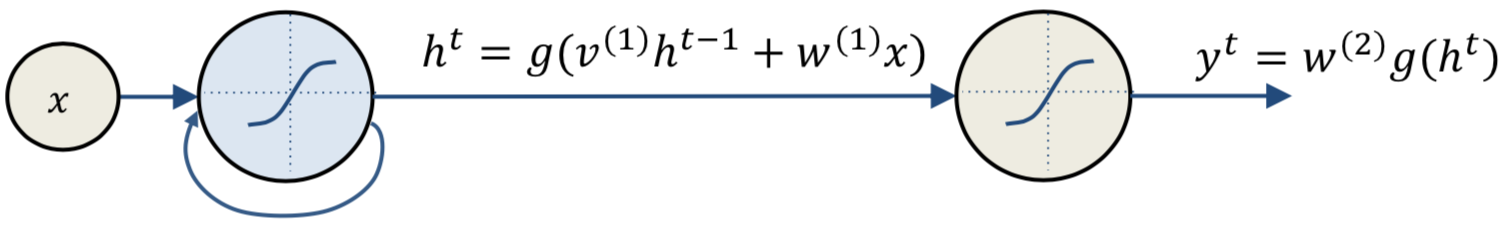
\includegraphics[width=15cm]{images/simplified_rnn.png}
        \label{fig:sim_rnn}
\end{minipage}
\vspace{0.2cm}

The model represented is a simplified model. Considering $v^{(1)}$, it is how much the output of this neuron is weighted to compute the next one.  The output of the hidden neuron is a non-linear function g() depending on the weighted sum of the previous loop $v * h^{t-1}$ plus a weighted input. %Then you have an output neuron. 
Focusing on the first part of the network, assume you want to derive the error w.r.t. input weight %this weight (quello dell'input) 
and you want to minimize the sum over all the sequences of the derivative of the error at time t w.r.t. to the weight of the input. This weight appears in the input but also in the previous inputs. So this derivative is not so easy, but we can use the trick of the chain rule of derivatives: 
%consider the sum over all possible sequences; take one of this sequence and find what is the error at time t w.r.t. the weights. This derivative is equal to the sum over all timestamps of the derivative wrt to the previous output, the derivative of the output w.r.t. to the input which is h at time t, times the derivative of this w.r.t the previous hidden value, times the derivative of it times the derivative value w.r.t. x (penso abbia guardato la figura più che la formula delle derivate). 
$$
\frac{\partial E}{\partial w}=\sum_{t=1}^{S}\left(\frac{\partial E^{t}}{\partial w}\right) \rightarrow {\frac{\partial E^t}{\partial w}} = \sum_{t=1}^{t} \frac{\partial E^t}{\partial y^t} \frac{\partial y^t}{\partial h^t} \frac{\partial h^t}{\partial h^k} \frac{\partial h^k}{\partial w}
$$
So basically, depending on how much is k, you derive w.r.t. to one of the past loops. If you look at the second formula, you notice that the derivative of the hidden neuron output w.r.t. any of the output in the past,  is $$
\frac{\partial h^{t}}{\partial h^{k}}=\prod_{t=k+1}^{t} \frac{\partial h_{i}}{\partial h_{i-1}}=\prod_{i=k+1}^{t} v^{(1)} g^{\prime}\left(h^{i-1}\right)
$$
i.e. the product of the derivatives from $k$ to $t$ of the derivative of time $t$ over $t-1$: 
%(guardare gli appunti per un esempio di questa parte)
%If you define the derivative as g'(), you see that this derivative is the product of:
%$$
%\frac{\partial h^{t}}{\partial h^{k}}=\prod_{i=k+1}^{t} \frac{\partial h_{i}}{\partial h_{i-1}}=\prod_{i=k+1}^{t} v^{(1)} g^{\prime}\left(h^{i-1}\right)
%$$
Note that the derivative of $g(v()*h)$ is $g^{\prime}()* v^{(1)}()$. %Non ne sono sicuro di quest'ultima frase
Considering the norm
$$
\left\|\frac{\partial h_{i}}{\partial h_{i-1}}\right\|=\left\|v^{(1)}\right\|\left\|g^{\prime}\left(h^{i-1}\right)\right\| \Rightarrow\left\|\frac{\partial h^{t}}{\partial h^{k}}\right\| \leq\left(\gamma_{v} \cdot \gamma_{g^{\prime}}\right)^{t-k}
$$
It means that the the norm is less or equal than the product of two terms: $\gamma_v$ is given by the weights, the other  $\gamma_{g^{\prime}}$ is given by the derivatives, and the exponent is how long is the past. \\
So if you go one step back, you see that this is the v*derivative, if you go 2 step back you have the product v derivatives * v*derivative: depending of the value of this term, you have a sequence of products which might go either to infinite or zerO. \\
In particular, if 
%(credo intenda la norma di delta $h^t$ fratto delta $h_k$)
$$ \rho = \left\|\frac{\partial h^{t}}{\partial h^{k}}\right\| < 1$$
%is less than 1, 
it converges to zero.
%because it is a number which is less then 1. 
%This is the gradient of the error at time $t$ wrt the weights,  the contribution of past inputs goes to zero.
If the derivative is less than 1, the gradient of the error function w.r.t. to an input $t-k$ steps back in the past goes to 0. \\
The point is that if you try to update the weight of an input $k$ epochs ago, your gradient is null. If you use for this weight either a \textit{tanh} or a \textit{sigmoid}, by definition $\gamma_{g^{\prime}}$ is less than 1. We have seen that the derivative of sigmoid and tanh, are respectively, $0.5$ or $0.25$: it means that in few steps in the past, the derivative of the output w.r.t. to the input will be 0 $\rightarrow$ With Sigmoids and Tanh we have Vanishing Gradient. \\
You may think that the other number $\gamma_{v}$ is going to compensate, but it means the more you go in the past, the more it should be bigger, but it make no sense: this value $\gamma_{v}$ is a constant. If it is a big constant such that the product is bigger than 1, it worst because you have that
%(norma di delta $h^t$ fratto delta $h_k$)
$\rho > 1$
%is greater than 1 to the 3 hundred-twenty, 
so the gradient will explode numerically. \\

%slide 15
The only solution is to force all gradient to be either 0 or 1, otherwise vanishing gradient or gradient explosion occur. 
The only way to perform is using \textbf{ReLu}: 
$$g(a) = ReLu(a) = max(0,a) \Rightarrow g^{\prime (a)} = 1_{a>0}$$ 

%The only possible value to set to this in order to not explode is 1, so you have to force for this loop the derivative of wrt the loop = 1, otherwise this term is greater than 1 explode, if less it vanishes. To force this loop to have derivative 1, since this loop is the derivative of the activation function, if you have an activation function for which the derivative is 1, you guarantee that you don't have vanishing gradient due to this step. You have to use ReLu. This not resolve the exploding gradient problem but if you initialize the weight small enough, the gradient will try to fit them without getting an explosion. 
This solve part of the story, no more vanishing gradient, but you have still the risk of exploding gradient. \\
If we force this loop to have weight = 1, we guarantee nor exploding or vanishing gradient because the derivative w.r.t. to the previous step will be always 1.\\
It is constraining the model by solving the vanishing gradient and the exploding gradient. By doing this you make the output dependent on whatever time you want. It is like a shortcut connection with all timestamps in the past.\\ \\
If you look closer, if the weight $v^{(1)}$ is = 1, you do not need to train the model; now this is a pure Feedforward Neural Network with all previous steps. This weight has not to be trained, for all those replicas you know already the weights, they are all 1, so no training is require for this loop.\\
This kind of object is called \textbf{Constant Error Carousel}.\\ By doing this the output depends on all the history of the input. The problem of the network is that it can \textit{only accumulate the input}, it just computes the integral of the input. \\This topology is useless because it is only integrating the input. 

%1:06:50
\subsubsection{Long-Short Term Memories}
Hochreiter \& Schmidhuber (1997) solved the problem of vanishing gradient designing a memory cell using logistic and linear units with multiplicative interactions. \\

\begin{wrapfigure}{l}{7cm}
    \includegraphics[width=7cm]{images/lstm_original.png}
    %\label{fig:lstm_org}
\end{wrapfigure} 

The creators started from the idea of Constant Error Carousel (CEC) and they thinks that now that we have an accumulator of the input, the only things to do is to build a network to learn when it is worth to add an input to the memory and when it is worth to read an input from the memory. \\ \\
The idea is to have some of \textit{gate} mechanism where:
\begin{itemize}
    \item[--] Information gets into the cell whenever its \textit{“write”} gate is on.
    \item[--] The information stays in the cell so long as its \textit{“keep”} gate is on.
    \item[--] Information is read from the cell by turning on its \textit{“read”} gate.
\end{itemize}{}
The gates are based on Constant Error Carousel. You can back-propagate through this since the loop has fixed weight. 

%To get out of the above issue,  is the idea of LSTM where the creators started from the idea of Constant Error Carousel and they said ok, now I have this CEC cell which is able to accumulate the input, what the network need to learn is when it is worth to add an input to the memory and when it is worth to read an input from the memory. The idea is to have some gating mechanism where you have this CEC, and you have a neural network which decides when it is useful to write in this memory and another network that decides when cancel or erase the memory and another network which decides when it is time to read from the memory.
Decision (e.g. as write/not-write) are based on the output of a Sigmoid; instead, the loop is ruled by a ReLu activation function. This kind of cell is the first \textbf{Long-Short Term Memories} idea. \\
The current architecture of the cell is shown below:

\vspace{0.2cm}
\begin{minipage}{\linewidth}
    \centering
    \includegraphics[width=15cm, height=4.5cm]{images/lstm.png}
    \label{fig:lstm}
    % \captionof{LSTM}
\end{minipage}
\vspace{0.2cm}

%This network [quella più a sinistra $net c_j$]  (in realtà penso più i gate che fanno accedere alla cella) have sigmoidal activation function which if says 0 you don't add anything in the memory, if 1 you add to the memory. The other network $net in_j$ decides what to add (+1 or -1), so these two modulate the content of the memory, based on the input: basing on the input it decides if store or not to or, if erase or not the memory.
%Nel mezzo c'è la Relu function which is a linear function, with the loop. Then there is the output of the network.
%Assume you have many of these cell and you output may depend on some of those. This cell is the first LSTM idea. 

%The nice thing is that you don't need unrolling because you can put many of these in the sequence and you can train without network unrolling because you don't need to train the weigth of the constant error carousel. 

%slide 17
%This is the architecture of RNN where at time t, the output of your network is a function of your current input and of your previous state. 

%slide 18
Different gates are highlighted:
\begin{itemize}
    \item[--] Input gate: the input is computed by the $tanh$ path and it is multiplied by this $sigmoidal$ part. It states if it is worth or not to write in the memory
    \item[--] Forget gate: in charge of re-writing or erasing the content of the memory. The memory is multiplied by a $sigmoid$, which indicates to keep the input if the sigmoid is equal to 1, otherwise erase the memory before adding the input. 
    \item[--] Memory gate: decide on adding the input to the previous state of your network. The memory is the sum of the forget gate and the input gate. 
    \item[--] Output gate: it is the combination of tanh and the reading mechanism controlled by a sigmoid. 
\end{itemize}{}

With LSTM networks you can build a computation graph with continuous transformation: the idea is that you can build an internal representation of the history of the input. This internal representation is updated at each input. \\
We can build different configurations of LSTM: 
\begin{itemize}
    \item One-to-One: translate one to one, one input and you want to translate it in another. For each input you predict one output
    \item One-to-many: one input and you want to predict many output. If x is the input, the idea is that the input modifies the state of the network and what happens is that you output one value, then another one, then another one. This kind of approach is used in Captioning: you enter an input (an image), you start with the first word, the you feed the model with this first word and you output the second word and so on; you write textual description for a single input. 
    \item Many-to-one: sequence of input and you want one output: example is Text Classification. 
    \item Many-to-many: it is in Video Classification or Video Captioning.
    \item Sequence-to-Sequence: you enter a sequence, then you have a state and the machine is started with this state. Then you generate a sequence. You think this kind of network as a sequence encoder. Since this model can be used also for generation, you have an input sequence and you use the state of this machine to generate a new sequence. This is the way most of text prediction and question answer are trained: you have a sequence encoder; once encoded this hidden representation for the sentence, you use a decoder (which is the same or a different LSTM) which is trained to output sequence conditioned on the value of this state. 
\end{itemize}{}

%Yo have different gates: 
%input gate: get the input
%the memory gate: you decide to add to the previous state of your network the input. The memory is the sum of the forget gate and the input gate

%The input is computed by the tanh path and it is multiplied by this sigmoidal part which says if it is worth or not to write in the memory

%Forget gate: in charge of rewriting or canceling the content of the memory. Decides whether it is worth to keep or decrease the content of the memory: you see that the memory is muliplied by a sigmoid which indicates to keep the input if the sigmoid is equal to 1, otherwise erase the memory before adding the input. 
%[Penso che i sigma siano i gate che sono fatti proprio da sigmoid function]

%Output gate is combined with some tanh and there is the reading mechanism which is this sigmoid multiplied by the gate.

%There is this forget gate: this network could learn to forget, but in order to do this it has to learn to remove content from the memory. So in the current implementation of LSTM, the forget gate is in charge of erasing partially the content of the network. 

\subsubsection{Gated Recurrent Unit}
An evolution of this memory is the \textbf{Gated Recurrent Unit}. It is more or less the same of LSTM: it combines the forget and input gates into a single "update gate". It also merges the cell state and hidden state, and makes some other changes.

%slide 24
%What can you do with LSTM: the idea is that they can build an internal representation of the history of the input. This internal representation is updated at each input. 
%At the beginning, we have this representation (slide24), you have an input, some hidden representation and the output is a function of this hidden representation. Then another input modifies the hidden layer and so on. 

%slide 25
%Se coloriamo le varie parti, we can build some different configuration of LSTM: 
%slide 26
%You can have mulitple LSTM layers. You have the input, then one LSTM which create a low level memory of the input, then another LSTM which remember an High level representation of the input, then you can have a non-linear function of the hidden layer as the output of the model

\subsection{Tips and Tricks}
Sometimes you can use \textbf{bidirectional LSTM}: if you have for instance many-to-one approach, you can read the sequence from left to right and vice-versa, put the two encoding together and classify the output with it. This is used often if you have to predict the output only having seen the entire sequence: you can process the sequence in the two direction. You cannot do it always, if you predict online, you cannot use it. \\

Another trick is in weight initialization:
\begin{itemize}
    \item Could initialize them to a fixed value
    \item Better to treat the initial state as learned parameters:
        \begin{enumerate}
            \item Start off with random guesses of the initial state values
            \item Backpropagate the prediction error through time all the way to the initial state values and compute the gradient of the error with respect to these
            \item Update these parameters by gradient descent
        \end{enumerate}{}
\end{itemize}

%you have to initialize the state of the network to a given state. One possible way is to initialize to an fixed value. It can be interest when you learn the network, to learn also the initial state of the network.
\section{Sequence2Sequence}
% output of LSTM is a non-linear function of the memory, which is the result of the writing and the forget gates. 
Some examples based on the input/output sequence:
\begin{itemize}
    \item One-to-many  - \textit{Image Captioning}: input a single image and get a series or sequence of words as output which describe it. The image has a fixed size, but the output has variable length
    
    \item Many-to-one - \textit{Sentiment Classification/Analysis}: input a sequence of characters or words, e.g., a tweet, and classify the sequence into positive or negative sentiment. Input has variable lengths, output is of a fixed type and size. You accumulate the inputs until the last LSTM, which states an output. 
    \item Many-to-many - \textit{Language Translation}: having some text in a particular language, e.g., English, we wish to translate it in another, e.g., French. Each language has it’s own semantics and it has variable lengths for the same sentence. Can be done in two ways: accumulating the inputs through hidden states or answering directly. The second looks like more natural, but it has some drawbacks: you need that translation can be treat as an aligned process, it works if the input and the outputs are synchronized. Most of Sequence2Sequence model works like the first one.
\end{itemize}{}

The Seq2Seq model follows the classical encoder decoder architecture: at training time the decoder \textbf{does not} feed the output of each time step to the next; the input to the decoder time steps are the target from the training. At inference time the decoder feeds the output of each time step as an input to the next one.

\begin{minipage}{\linewidth}
        \centering
        \includegraphics[width=13cm, height=5cm]{images/s2s.png}
        %\captionof{figure}{The model pipeline.}
        %\label{fig:flow_fig}
\end{minipage} \\

%slide 8
%A,B,C is the question, WXYZ is the answer. 
%Once you have learned A B C and you start the output, basing on an special symbol, you output W. Then X is the most likely answer after have been seen A B C D and W. 
%The <eos> is triggered by how you build and modify the state via the answer. 

%slide 9 
At training time, you write the input with no target [the green part]. Only when you input the $<GO>$, you start with the target. Then in order to predict the second target, you feed your network with the previous target.\\
Once the model is trained, you give the input, which ends with $<GO>$ and the model starts to predict the most likely output. As before, once the output is computed, in order to predict the next output, the previous one is given as input. When the network see $<eos>$ is terminates. \\
Each sequence can have different lenght, but you can enforce a maximum length for the output. 
\\
Word Embedding means represent the same word in less sparse representation. The yellow part (the one in the bottom) transforms words into vector , the other yellow part (the one in the top) reverse the process. 
Because of the embedding, the output is the selection among the possible words that it should say as output: usually it is a softmax output among all possible output words. \\

%There are different way to encode into text: bi-grams, tri-grams and so on. This is interesting since tri-grams are less than the number of words in the vocabulary because the pairs of letters. The nice thing is that once you have all the bi-grams or tri-grams you can write all the words in the vocabulary. In principle, also the words that are not in training set. 
Special characters:
\begin{itemize}
    \item[--]$<PAD>$: During training, examples are fed to the network in batches. The inputs in these batches need to be the same width. This is used to pad shorter inputs to the same width of the batch
    \item[--]$<EOS>$: Needed for batching on the decoder side. It tells the decoder where a sentence ends, and it allows the decoder to indicate the same thing in its outputs as well.
    \item[--]$<UNK>$: On real data, it can vastly improve the resource efficiency to ignore words that do not show up often enough in your vocabulary by replace those with this character.
    \item[--]$<SOS>$/$<GO>$: This is the input to the first time step of the decoder to let the decoder know when to start generating output.
\end{itemize}

%slide 10
%Once you have trained your model at runtime, what you do is this. You give the input which ends with GO. So the model start to predict the most likely output. Then this is inputted to the second one and so on. When the network says <eos>, it stops. 
%Each sequence can have different length and you can at runtime enforce a maximum length for the output. 

Sometimes the first best results is not the real best. Usually if you take the second best, the sequence goes better. So you can do what is called \textit{Beam Search} (?): take the first 3 results, then you run three parallel executions. Considering the results of these execution, you choose the best one according to some criteria. \\

%Sometimes the first best is not the best. Usually if you take the second best, usually the sequence goes better. So what you do is what it is called Beam Search [?]: you take the first 3, then you run three parallel execution. Then you get the three more likely and you look three step ahead and you have some criteria to select which will be the best answer. 

Dataset Batch Preparation:
\begin{enumerate}
    \item Sample $batch\_size$ pairs of ($source\_sequence$, $target\_sequence$).
    \item  Append $<EOS>$ to the $source\_sequence$
    \item Prepend $<SOS>$ to the $target\_sequence$ to obtain the $target\_input\_sequence$ and append $<EOS>$ to obtain $target\_output\_sequence$.
    \item  Pad up to the $max\_input\_length$ ($max\_target\_length$) within the batch using the $<PAD>$ token.
    \item Encode tokens based of vocabulary (or embedding)
    \item Replace out of vocabulary (OOV) tokens with $<UNK>$. Compute the length of each input and target sequence in the batch.
\end{enumerate}{}


%slides 11
%Sometimes you have special characters. 

%slides 12 
%This is how you prepare the batch of words. 

%slide 13
In order to compute the error, you have to compute the probability of one character given the state $v$ and the outputs. Given $<S, T>$ pairs, read $S$, and output $T^{\prime}$ that matches $T$: 
$$
\begin{aligned}
p\left(y_{1}, \ldots, y_{T^{\prime}} | x_{1}, \ldots, x_{T}\right) &=\prod_{t=1}^{T^{\prime}} p\left(y_{t} | v, y_{1}, \ldots, y_{t-1}\right) \\
1 /|\mathcal{S}| & \sum_{(T, S) \in \mathcal{S}} \log p(T | S)
\end{aligned}
$$

%You try to minimize the error of the target sequence given the input sequence. To do this, you compute this error as the probability of one character given this state (the encoding) and the previous output: formula

So you can train this model with Cross-Entropy. You can image that each of these networks are softmax over a specific word; you sum the cross-entropy over the sequences and you minimize by the network estimates. So  backpropagate on the cross entropy, trying to get the exact sequence. \\

%slide 14
In general you can stack multiple layer of LSTM: you might have a sort of hierarchical representation. You can perform this embedding hierarchy but through time and then you can have some non-linear transformation (ReLU) at the top. You can also have shortcut connections.\\ 

\paragraph{Bidirectional LSTM}
You can have two level, one goes forward, the other backward through the LSTMs and then you concatenate the LSTMs and you predict the output. The point is: let's assume you want to predict for each word in the sentence if that word is used in positive or negative way in the sentence. If we do it in one direction only, the output depends only on the previous ones. But if the mean of that word change through the sentence, for each word in might be useful what will be after. \\ \\ 

The Sequence2Sequence idea has possible drawbacks: you are compressing long sequences into a vector. It works, backpropagation does not suffer the vanishing gradient, but you can have problem in processing long sequences. The way Seq2Seq is done, the way embedding of sequence into a state and decoding this embedding in another sequence is done, has still some limitation into how much information and how much knowledge or context you can embed into this vector.\\
After a few tests on LSTM people tried to add memory to recurrent neural Networks: it can be achieved in different ways, the most interesting one is the so called \textbf{Neural Turing machine}.

\subsection{Neural Turing machine}
%After a few tests on LSTM people tried to add memory to recurrent neural Networks.
%What does this mean? It can be achieved in different ways, the most interesting one is the so called \textbf{Neural Turing machine}. 
If you remember, in Turing machine you have a infinite
string of symbols
%, reading and writing, 
and you can perform any computation by a series of operations that reads and writes in a sequence from this string. We can do it with the neural network in
the sense that what this recurrent model does is basically storing information in the
memory, reading from it and writing in it. It uses the memory
explicitly 
%(explicit use) 
instead of an encoding of it.\\
So \textbf{Neural Turing Machines} combine a RNN with an external memory bank. \\

\begin{minipage}{\linewidth}
        \centering
        \includegraphics[width=15cm, height=5cm]{images/ntm.png}
\end{minipage} \\ 

I’m using an NTM mostly because the trick used in NTM to read and write for the memory is probably the most interesting part and it’s the same trick upon which we base the attention mechanism. \\
In the figure, you have a network which can write or rewrite the memory given some input; you decide to modify the first cell to store this input and then you read the next step; you get another input and you decide to write the second based on the state of the memory; the same for the third and fourth and so on and so forth. \\
In general, especially when you have long sequences, you would like to partition your memory in states and you would like to use this memory to do things.\\
The problem is that \textit{read} and \textit{write} are \textit{not differentiable} operations.\\
Think about read: reading  means you select one address and extract the cell and only the cell at a specific address; in the same way, writing means you select one address and you change the content of that address.\\
So while writing and reading per se are easy to differentiate, \textit{addressing} is the problem. We would like to learn where to write. Memory addresses are discrete by definition so you should be able to derive
the write and read operation with respect to the address. This
seems a very complex issue which has a very simple solution: \textit{write always everywhere}.\\

Neural Turing Machine challenge:
\begin{itemize}
    \item[--] We want to learn what to write/read but also where to write it
    \item[--] Memory addresses are be fundamentally discrete
    \item[--] Write/read differentiable w.r.t the location we read from or write to
\end{itemize}{}
The solution is: \textit{every step, read and write everywhere, just to different extents} [Attention mechanism]. \\ 
%This way you don’t have to have many recurrent complex things but what you have to do is to learn the sequence of operation read-write-read-write and what to write into. Another mechanism to have memory is somehow not to compress the entire sequence into a single state but to somehow allow the decoding process to \textit{go back} and read what was written in the input, so you have each word in the output depend on each word in the input. This is done with the so called \textbf{attention mechanism} and I would like to discuss the NTM and the attention interfaces. 
%Actually I am more interested in the latter but turns out that introducing NTMs implies an understanding of attention interfaces. 

\begin{minipage}{\linewidth}
        \centering
        \hspace*{-2cm}    
        \includegraphics[width=18cm, height=5cm]{images/attention.png}
\end{minipage} \\ \\

%NTM combines recurrent neural networks with memory bank. So basically you have this recurrent neural network, it could be an NTM or a classic recurrent neural network, and make sure you can store enough information in the memory, so you decide that instead of having a set of vectors you have a memory of vectors, so each of these cells contains a vector so that the state would not be one vector summarising the sequence of input so as to average the sequence of input but to be n vectors, and each of them has stored a function of the input and modify this content in a recursive way. For example, assume I get one vector and then I get 7 vectors I don’t need, then a second, then another vector which is the sum of the past 2 vectors combined with the new one; this kind of operation requires to store an input at some point in some place, then store another one and then conditionally get these two, sum the two and put them back. Implementing this, a non linear function of a non linear function of a non linear function, is not necessarily easy to do. 

%Let me get the \textit{translation example}; it’s obvious you want to translate text from one language to another and it’s easy if you have a short context to keep in memory but if you want to memorise 10 pages of text and then translate it exactly from time to time it’s like "okay let me read the first one, let me write some notes here, then let me read the second and write some notes here, then I read the third and write some other notes..." and after I read the notes and I translate the notes instead of writing a single content. So this is a way to increase the memory and the expressivity of the content. This will be very helpful also with respect to NTM and Sequence to Sequence encoding.  I’m using an NTM mostly because the trick used in NTM to read and write for the memory is probably the most interesting part and it’s the same trick upon which we base the attention mechanism. 

%So let’s see here you have a network which can write or rewrite the memory so basically you have some input, you decide to modify this cell to store this input and then you read the next step, you get another input and you decide to write the second based on the state of the memory, then the third and fourth and so on and so forth. In general, especially when you have long sequences, you would like to partition your memory in states and you would like to use this memory to do things.

%If you think about the reversed string or reversed text, it becomes very easy this way. If you want to write a string in reverse order then it’s more complex because the context has to store the \textit{sequence} of words you have used plus the \textit{order} you have used, and if the model is a reversed model string, you cannot imagine that in the training set you have all the strings and the reversed ones. So basically, to learn an LSTM reversible string is much more difficult than to learn an NTM reversible string; what you have to do is write from left to right when you see the go symbol (non so perché lo dica) read from right to left and you have reversed it, so it’s easier and quite straightforward to implement reversed string, so writing and learning algorithms is easier. 

%The problem is that read and write are not differentiable operations. Think about read, reading  you select one address and extract the cell and only the cell at a specific address, write you select one address and you change the content of that address.
%So while writing and reading per se are easy to differentiate, \textit{addressing} is the problem. We would like to learn where to write.

%Memory address are discrete by definition so we should be able to derive the write and read operation with respect to the address. This seems a very complex issue which has a very simple solution: \textit{write always everywhere}.

%How much you decide to write depends on the input. In each step, I write everything but mostly in some cells, so it means that based on my input I will write in this cell and not in that one. It’s a sort of associative writing but in principle at each step I could write everywhere. Think about LSTM gates, the idea is the same, in each cell you decide where and what to write, here the gate is over the entire memory and you decide on all the cells ‘on this I write on this I don’t’. So the idea is to have an \textbf{attention mechanism}: basically your data will tell you where to write, so that it puts your attention on specific cells. You have your memory and this is the ‘read’ so you say you have to read from this cell so you put attention here. 

How much you decide to write depends on the input. In each step, I write everything but mostly in some cells, so it means that based on my input I will write in a cell and not in another one. It’s a sort of \textit{associative writing} but in principle at each step I could write everywhere. \\
Thinking about LSTM gates, the idea is the same: in each cell you decide where and what to write; here the gate is over the entire memory and you decide on all the cells to which cell to write or not to write.\\
%‘on this I write on this I don’t’. 
So the idea is to have an \textbf{Attention mechanism}: basically your data will tell you where to write, in order to put your attention on specific cells. \\
In the left part of the Figure, you have your memory and a ‘read’: you want to read from a particular cell, thus you put attention there. \\
Two types of attention: 
\begin{itemize}
    \item[--] \textbf{Content-based attention}: searches memory and focus on places that match what they're looking for
    
    \item[--] \textbf{Location-based attention}: allows relative movement in memory enabling the NTM to loop
\end{itemize}{}

\begin{minipage}{\linewidth}
        \centering
        \hspace*{-2cm}    
        \includegraphics[width=14cm, height=8cm]{images/attention_example.png}
\end{minipage} \\ \\

Think about having a softmax output: 
%\begin{center}
%    \includegraphics[width=0.6\textwidth]{images/attentionsoft.PNG}\par
%\end{center}
%it has some peaks which are very close to 1, so basically if this is the softmax of a neural network, given a certain input you can select with this softmax which cell you’re gonna read; what happens is that the reading would be the weighted average where the weights are the softmax weights of your entire reading. Because the softmax is very selective (it’s a normalised exponential function) you would read mostly from one or two or three cells, and if for some reason you would read from 3 because you can still retrieve multiple cells from the memory and the interesting part is that you can derive this because it is nothing but the product between the memory, which is nothing more than a set of vectors, and the attention which is a softmax and it's differentiable. Each item is thus weighted with the query response to produce a score.

Basically, given a certain input you can select with this softmax which cell you’re gonna read; what happens is that the reading would be the weighted average where the weights are the softmax weights of your entire reading. \\
Because the softmax is very selective (it’s a normalised exponential function - it's almost everywhere equal to 0) you would read mostly from one or two or three cells 
%,and if for some reason you would read from 3 because you can still retrieve multiple cells from the memory 
and the interesting part is that you can derive this because it is nothing but the product between the memory, which is nothing more than a set of vectors, and the attention, which is a softmax and it is differentiable.\\
Each item is thus weighted with the query response to produce a score.\\


%So if you have 1 0 0 0, this way you only replace the memory cell. Let’s assume you have 0,5 here and 0,5 here, you merge this cell with the new value, this cell with the new value, and at the end the part is left unchanged. You didn’t really select those 2, you wrote everywhere but since this softmax is almost everywhere equal to 0, its almost like selecting some specific cells. Once you learn the trick it’s pretty simple. Now you can jump multiple vector stored and you don’t have necessarily each of them to depend on the history of the network, plus you can have attention memory which depends on the input. SO let’s put this into an entire network.


%Let’s assume that you have your memory and some input vector. This input vector to some extent should trigger the cell in the memory you want to write into. So for instance you might decide this query vector is retrieving which cells are most similar to this input. So you would change the memory cells which are more similar to this input. Based on this you have a similarity pick, then a softmax layer on this similarity pick, which will select which one is the current attention, the current cell you want to put attention on. Sometimes the attention depends not only on the current input but also on the previous input, so let’s assume you want to learn to look around so my attention goes first there, now it should go there again but since I have already looked there i’ll go there (forse è un diverso there) because you want to move or interpolate your attention mechanism to somehow have a local smoothness. You have this interpolation which is a parameter between the old attention and te new attention, this parameter will tell you how much to shift your attention from one timestamp to the other, then you have this attention that can have a shift .. so you only move the focus, you don’t jump, you chase the focus instead of jumping from one place to another, you sharpen because you want the minimum amount of cells. SO after these operation you have decided which are the cells to write in. This is a complex implementation of what I said before. 
Based on the input, you have a softmax on the memory and the output gets changed based on this memory. The softmax is driven by the input, so it’s a content-based attention, and once you have retrieved the most similar area in the memory, you have a sort of location-based mechanism 
%not to jump from one location to another 
and this location mechanism allows you to move from one area to another.\\ 

%Now, this is what I wanted to talk about for Turing Machines, I don’t really want to get into this sort of different architectures, but 
What is interesting and relevant of NTM is the idea that you can \textbf{focus on a PART} of your memory: this is \textbf{Attention}!\\
%It’s better than LSTM in remembering long sentences, they can learn how to look in sequences, to sort or reverse numbers, something which is not easy in lstm because you have to encode the order in one single-context vector while here you don’t need to do that because the memory sorts things, and there are many improvements on Neural Tuning machines, but, besides this improvements, what I’m interested in is Attention. Probably the most relevant outcome of NTM in these models is the idea that you can avoid mixing things by storing them and to focus or weight these memory cells.


\subsubsection{Attention Mechanism in Seq2Seq Models}
So people realized that the attention mechanism could have been an interesting add-on for the Sequence to sequence model I was talking about before. \\

%So people realized that the attention mechanism could have been an interesting add-on for the Sequence to sequence model I was talking about before. Why? Let me make an example so make it clear. Lets consider a set of sequences with a set of inputs and a set of outputs, the decoder (the sequence generator) has the goal of generating this sequence of output starting from the input which is the context, and this is the summary of the sequence. If you do a standard vanilla seq2seq model, which is what we have discussed so far, your decoder is conditioned on the initial state which is the last state of the encoder (slide 23). For a short or medium-length input it works quite well, but if you have long sequences what happens is that you might have a problem at this point because you have squeezed all the information into one single vector and you might want to do it a little bit more flexible and more structured as you were doing with memories. So the trick is I don’t have a memory but I have a past, so instead on condition only on this state, I would have to condition this on the output of this on the output of this, I condition my sequence of words based on the words that had in the (event). 

Considering the sequential dataset $
\left\{\left(\left(x_{1}, \dots, x_{n}\right),\left(y_{1}, \dots, y_{m}\right)\right)\right\}_{i=1}^{N}
$, the decoder role is to model the generative probability: $P(y_1, ..,y_m | x)$.\\
In "vanilla" seq2seq models, the decoder is conditioned initializing the initial state with last state of the encoder. That works well for short and medium-length sentences; however, for long sentences, becomes a bottleneck.\\
Let's use the same idea of Neural Turing Machines to get a differentiable attention and learn where to focus attention.\\ 

\begin{minipage}{\linewidth}
\centering
\hspace*{-2cm}    
\begin{minipage}{9cm}
  \includegraphics[width=9cm, height=7cm]{images/attentionsoft.PNG}
  %\captionof{figure}{A figure}
  %\label{fig:test1}
\end{minipage}%
\begin{minipage}{10cm}
  \centering
  \includegraphics[width=10cm, height=4cm]{images/attentionsoft_right.png}
  %\captionof{figure}{Another figure}
  %\label{fig:test2}
\end{minipage}
\end{minipage}\\ \\

Attention distribution is usually generated with content-based attention.\\
Each item is thus weighted with the query response to produce a score. Scores are fed into a softmax to create the attention distribution

Attention function maps query and set of key-value pairs to an output. \\
Output computed as a weighted sum of the values, where the weight assigned to each value is computed by a compatibility function:


\begin{enumerate}
    \item Compare current target hidden state $\boldsymbol{h_t}$ with source states $\boldsymbol{h_s}$ to derive attention 
    $$
    \operatorname{score}\left(\boldsymbol{h}_{t}, \overline{\boldsymbol{h}}_{s}\right)=\left\{\begin{array}{l}
    {\boldsymbol{h}_{t}^{\top} \boldsymbol{W} \overline{\boldsymbol{h}}_{s}} \\
    {\boldsymbol{v}_{a}^{\top} \tanh \left(\boldsymbol{W}_{1} \boldsymbol{h}_{t}+\boldsymbol{W}_{2} \overline{\boldsymbol{h}}_{s}\right)}
    \end{array}\right.
    $$
    
    \item Apply the softmax function on the attention scores and compute the attention weights, one for each encoder token
    $$
\alpha_{t s}=\frac{\exp \left(\operatorname{score}\left(\boldsymbol{h}_{t}, \overline{\boldsymbol{h}}_{s}\right)\right)}{\sum_{s^{\prime}=1}^{S} \exp \left(\operatorname{score}\left(\boldsymbol{h}_{t}, \overline{\boldsymbol{h}}_{s^{\prime}}\right)\right)}
$$
    
    \item Compute the context vector as the weighted average of the source states
    $$
    \boldsymbol{c_t} = \sum_{S} \alpha_{ts}\boldsymbol{ \overline{\boldsymbol{h}}_s}
    $$
    \item Combine the context vector with current target hidden state to yield the final attention vector
    $$
\boldsymbol{a}_{t}=f\left(\boldsymbol{c}_{t}, \boldsymbol{h}_{t}\right)=\tanh \left(\boldsymbol{W}_{c}\left[\boldsymbol{c}_{t} ; \boldsymbol{h}_{t}\right]\right)
$$
\end{enumerate}{}

\begin{minipage}{\linewidth}
\centering
\hspace*{-2cm}    
\begin{minipage}{9cm}
  \includegraphics[width=9cm, height=7cm]{images/attention_mechanism.jpg}
  %\captionof{figure}{A figure}
  %\label{fig:test1}
\end{minipage}%
\begin{minipage}{10cm}
  \centering
  \includegraphics[width=9cm, height=8cm]{images/bahdanau-fig3.png}
  %\captionof{figure}{Another figure}
  %\label{fig:test2}
\end{minipage}
\end{minipage}\\ \\


%SO basically if I translate ‘ I AM A’ if I have to translate the next word I would like to look at what’s written here, it’s like a memo. (24:16) So basically the idea is to have a sort of network mechanism, when you decode you are allowed to use input as the memory, so you start by looking at the sort of summary of the sentence but then you have to go back and say what was that for? Because this is available to your decoder, you have the input and the entire sequence and after looking after initialising this sequence you can add to the current state some input which was the past encoding so it’s like this: you have the first word, you encode it, you get the last word, you encode it, and then at each step you have a sort of attention mechanism based on current decoder which retrieves the last word, so to predict the next word you use the current state plus you retrieve like the reading mechanism from the past encoding a sort of more focused context. It’s like saying okay I get the point on the meaning of the text, I start writing and then from time to time when you are writing you look around you scatter around the previous text to say like ‘okay this I wrote this I wrote this I wrote’. With the images (quella sopra) this becomes clear immediately, think about capturing, you want to capture this ‘the cat is on’ and you look below the ‘cat’ and you say ‘table’, you focus on the part of the image which is always available and is relevant at that point. You do this starting from the central pick, the center, you would never describe the table is below the cat, you start from the cat which is in the center. So you have a sequence which is this internal state which tricks input in generating this (new sequence). Let’s see a simulation of this attention mechanism. 
%As you can see, you do exactly what’s written here, you do these replicas and so on and so forth, but you have also some connection here which are weighted, it’s a weighted sum with weights which are based on the content of the previous state. So the idea is the attention is a sort of content based (addressee? address?), so based on this value you retrieve the information in one sense. Based on your current state here you can retrieve the past, then you build a context vector which is not the very last but it’s based on attention, then you move forward and your attention changes, then you move forward again and you attention changes and so on. You keep the input as a memory. At this point you get I AM A STUDENT, the attention is on the second word, AM and JE but the trick is that you look back, at each step you know on which word you are putting your attention.

%So the idea is you have the current target in the state with the source state and you have a sort of attention, compare this with this and you use this to compare which is the most relevant out of these. You have some possible ways of computing the score. Given your final context you can retrieve a score between this context and the past. For instance, what is the most relevant score in the past based on this sequence, and then you build a context vector by mixing.. so from this core you built an attention mechanism, it’s not particularly complex in this case, then once you have the score between this and all the hidden states, a softmax, you build a context vector as the weighted sum of all these (contexts), so you use the last context to retrieve what word was the most relevant state and you build a new state as a new context, so you put your attention in generating the sentence, for instance you start here: the first one would be ‘I’ so you put a set of weights, your attention is on ‘I’ and ‘Je’, then you get Je, you change this state, you look here what is the most interesting word to go here, and it’s this so you get the hidden representation on AM, so basically by doing this you can jump back and forth, this jump is related to the current context, it’s related to the input and the output. How to retrieve is.. by doing this basically what happens is these two matrixes are used to compute ——- (sembra dica ‘are learned’) and this (———) so to know how to put your attention based on the history based on the train set on the input. Then you combine your hidden with this context, so you keep, so it’s just an add-on on the classic Sequence2Sequence and you go on forward. What you can do is at each time look at this vector and at the weights on this vector. 

The Figure on the right represents the \textbf{Alignment matrix}, used to visualize attention weights between \textit{source} and \textit{target} sentences. \\
For each decoding step, i.e., each generated target token, describes which are the source tokens that are more present in the weighted sum that conditioned the decoding. \\
We can see attention as a tool in the network’s bag that, while decoding, allows it to pay attention on different parts of the source sentence.

\begin{minipage}{\linewidth}
        \centering
        \hspace*{-2cm}    
        \includegraphics[width=17cm, height=5cm]{images/attention_example_french.png}
\end{minipage} \\

Attention allows processing the input to pass along information about each word it sees, and then for generating the output to focus on words.
Attention can be used in different scopes:
\begin{itemize}
    \item[--] Translation
    \item[--] Voice Recognition: attention allows one RNN to process the audio and then have another RNN skim over it, focusing on relevant parts as it generates a transcript.
    \item[--] Image Captioning: a CNN processes the image, extracting high-level features. Then an RNN runs, generating a description of the image based on the features. As it generates each word in the description, the RNN focuses on the CNN interpretation of the relevant parts of the image.
\end{itemize}{}

\subsubsection{Attention in Respose Generation - Chatbots}
Chatbots can be defined along at least two dimensions:
\begin{itemize}
    \item \textbf{Core Algorithm}:
    \begin{itemize}
        \item \textit{Generative}: encode the question into a context vector and generate the answer word by word using conditioned probability distribution over answer’s vocabulary. E.g., an encoder-decoder model.
        
        \item \textit{Retrieval}: rely on knowledge base of question-answer pairs. When a new question comes in, inference phase encodes it in a context vector and by using similarity measure retrieves the top-k neighbor knowledge base items.
    \end{itemize}{}
    
    \item \textbf{Context Handling}:
    \begin{itemize}
        \item \textit{Single-turn}: build the input vector by considering the incoming question. They may lose important information about the history of the conversation and generate irrelevant responses
        $$ {(q_i, a_i)}$$
        
        \item \textit{Multi-turn}: the input vector is built by considering a multi-turn conversational context, containing also incoming question  
        $$
        \left\{\left(\left[q_{i-2} ; a_{i-2} ; q_{i-1} ; a_{i-1} ; q_{i}\right], a_{i}\right)\right\}
        $$
    \end{itemize}{}
\end{itemize}{}

Vinyals and Le, 2015 and Shang et al., 2015 proposed to directly apply sequence to sequence models to the conversation between two agents:
\begin{enumerate}
    \item The first person utters “ABC”
    \item The second person replies “WXYZ”
\end{enumerate}{}

Generative chatbots use an RNN and train it to map “ABC” to “WXYZ”: we can borrow the model from machine translation; a flat model simple and general; Attention mechanisms apply as usual. \\

\textbf{Generative Hierarchical Chatbots} The idea could be concatenating multiple turns into a single long input sequence, but this probably results in poor performances. \\
LSTM cells often fail to catch the long term dependencies within input sequences that are longer than 100 tokens.\\
No explicit representation of turns can be exploited by the attention mechanism.\\

Xing et al., in 2017, extended attention mechanism from single-turn response generation to a hierarchical attention mechanism:
\begin{itemize}
    \item Hierarchical attention networks (e.g., characters $\rightarrow$ words $\rightarrow$ sentences)
    \item Generate hidden representation of a sequence from contextualized words
\end{itemize}{}

(Hierarchical Generative Multi-turn Chatbots - Hierarchical Document Classification guardare le slide) \\

\textbf{Attention is all you need} Having seen attention is what makes things working you start wondering: 
\begin{itemize}
    \item[--] Sequential nature precludes parallelization within training examples, which becomes critical at longer sequence lengths, as memory constraints limit batching across examples.
    
    \item[--]Attention mechanisms have become an integral part of compelling sequence modeling and transduction models in various tasks. Can we base solely on attention mechanisms, dispensing with recurrence and convolutions entirely?
    
    \item[--] Without recurrence, nor convolution, in order for the model to make use of the order of the sequence, we must \textbf{inject} some information about the relative or absolute position of the tokens in the sequence.
\end{itemize}{}
There has been a running joke in the NLP community that an \textbf{LSTM with attention} will yield \textit{state-of-the-art} performance on any task.
Attention is built upon RNN, .. The \textbf{Transformer} breaks this assumption!

\subsubsection{Transformer}
\begin{wrapfigure}{r}{7cm}
    \includegraphics[width=7cm]{images/The_transformer_encoder_decoder_stack.png}
\end{wrapfigure} 

In a Transformer model we can distinguish an encoding component, a decoding component, and connections between them. \\
The Encoders are all identical in structure (yet they do not share weights). Each one is broken down into two sub-layers:
\begin{enumerate}
    \item \textit{Self-Attention}: a layer that helps the encoder look at other words in the input sentence as it encodes a specific word
    \item \textit{Feed Forward Neural Network}: The outputs of the self-attention layer are fed to a feed-forward neural network. The exact same feed-forward network is independently applied to each position [\textbf{Position-wise Feed-Forward NN}]
\end{enumerate}{}
The Decoder has the following layer:
\begin{enumerate}
    \item \textit{Self-Attention}: as before
    \item \textit{Encoder-Decoder Attention}: helps the decoder focus on relevant parts of the input sentence
    \item \textit{Feed Forward Neural Network}: as before
\end{enumerate}{}

We begin by turning each input word into a vector using an embedding algorithm. The embedding only happens in the bottom-most encoder. \\
After embedding the words in our input sequence, each of them flows through each of the two layers of the encoder. Here we begin to see one key property of the Transformer, which is that the word in each position flows through its own path in the encoder. There are dependencies between these paths in the self-attention layer. The feed-forward layer does not have those dependencies. So the self-attention layer, in some way, stores the dependencies of inputs, while the Feed Forward is treated as 'independent' for each input.\\

\begin{wrapfigure}{r}[2cm]{8cm}
    \includegraphics[width=8cm]{images/transformer_self_attention_vectors.png}
\end{wrapfigure}

\textbf{Scaled Dot-Product Attention}\\
The \textbf{first step} in calculating self-attention is to create three vectors from each of the encoder’s input vectors: a \textit{Query vector}, a \textit{Key vector}, and a \textit{Value vector} [they are abstraction that are useful for the calculus]. These vectors are created by multiplying the embedding by three matrices that we trained during the training process. \\
Multiplying $x_1$ by the $W^Q$ weight matrix produces $q_1$, the "query" vector associated with that word. We end up creating a "query", a "key", and a "value" projection of each word in the input sentence. \\

The \textbf{second step} in calculating self-attention is to calculate a score: we need to score each word of the input sentence against this word. The score determines how much focus to place on other parts of the input sentence as we encode a word at a certain position. The score is calculated by taking the dot product of the query vector with the key vector of the respective word we’re scoring: so if we’re processing the self-attention for the word in position \#1, the first score would be the dot product of $q_1$ and $k_1$. The second score would be the dot product of $q_1$ and $k_2$. \\

The \textbf{third} and \textbf{forth steps} are to divide the scores by the square root of the dimension of the key vectors $\sqrt{d_k}$: this leads to having more stable gradients.\\
Then pass the result through a softmax operation. Softmax normalizes the scores so they’re all positive and add up to 1. \\

The \textbf{fifth step} is to multiply each value vector by the softmax score: the intuition here is to keep intact the values of the word(s) we want to focus on, and drown-out irrelevant words (by multiplying them by tiny numbers like 0.001, for example) \\

The \textbf{sixth step} is to sum up the weighted value vectors. This produces the output of the self-attention layer at this position (for the first word). \\

At the end the \textit{Attention} can be expressed as $$ Z = 
\text { Attention }(Q, K, V)=\operatorname{softmax}\left(\frac{Q K^{T}}{\sqrt{d_{k}}}\right) V
$$

\begin{wrapfigure}{r}[2cm]{5cm}
    \includegraphics[height=5cm]{images/multihead.png}
\end{wrapfigure}

\textbf{Multi-head Attention} If we do the same self-attention calculation we outlined above, just $h$ different times with different weight matrices, we end up with $h$ different Z matrices. \\
The feed-forward layer is not expecting $h$ matrices – it’s expecting a single matrix (a vector for each word). So we concat the matrices then multiple them by an additional weights matrix $W^0$ (which was trained jointly with the model). \\
The result would be the Z matrix that captures information from all the attention heads: this matrix is sent to the FNN.\\

\textbf{Positional Encoding} One thing that’s missing from the model as we have described it so far is a way to account for the order of the words in the input sequence. To address this, the transformer adds a vector to each input embedding. These vectors follow a specific pattern that the model learns, which helps it determine \textbf{the position} of each word, or the distance between different words in the sequence. The intuition here is that adding these values to the embeddings provides meaningful distances between the embedding vectors once they’re projected into Q/K/V vectors and during dot-product attention. \\ \\

To sum up, a Transformer model is made out of:
\begin{itemize}
    \item Scaled Dot-Product Attention
    \item Multi-head Attention
    \item Position-wise Feed-Forward Networks
    \item Embeddings and Softmax
    \item Positional Encoding
\end{itemize}{}
Self-Attention has $O(1)$ maximum path length; when $n < d$, Self-Attention has lower complexity per layer.


%So this is called Alignment Matrix (slide 27) and provides you with this alpha value as a function of the input, the sequence. So in the beginning the attention is on ‘L’ACCORD SUR LA ZONE’.. ehm reading French is still torturing (LOL).. so let’s read it this way ‘THE AGREEMENT ON THE EUROPEAN ECONOMIC AREA WAS SIGNED IN AUGUST 1992’, you want to translate this in French so you don’t have to read it (lol) so basically the first term you want to put your attention on is THE and you get this (L’). Now that you have written this, the second term you want to put your attention is AGREEMENT, then you translate it (ACCORD), then the next word you put attention on is ON (SUR) and then THE (LA) and now your attention ‘European economic area’ it’s interesting because in English you have the typical reversion (inversion magari) between name and adjective, so you want to focus on AREA which is economic of Europe. If you think of translating this into Italian, the first word you want to translate is AREA, not European. And the same is in French. Next time I will translate into Italian so I know how to read it properly *laughs* some other people was probably more proficient in French than me. So you see that now the attention based on the past is on this term because the way you do it is more clear if you translate from French to English. Let’s do it in Italian LA ZONA ECONOMICA EUROPEA: LA is an article, it’s female, and it refers to a noun; the next noun is ZONA, so I have to put my attention on this; and then I put my attention on the adjective and then this (prima ‘economica’, poi‘europea’). But in English they get reversed so by this mechanism you see that you can look at some groups of words A E’TE’ = WAS SIGNED, in August... this is related to the mere alignment of text. SO you see that you are able to focus on different parts of the sentence so most of the time the attention is on a group of letters which are useful to predict which is the right. So here you see you try, you kind of learn the alignment between the text and more interesting is that this very nice demo but I won’t speak about this demo we will come back on this later, you can do this with images as well: so for instance, let’s assume you want to produce caption, this same mechanism, let me do it this way.. when you have a sentence.. if you do captioning here you have the image, right? (forse sta disegnando qualcosa alla lavagna) and here you have the encoding or the cnn output of the image. You start with the first term and based on that now only a part of the image is relevant, you focus your attention on part of the image. Then when you have processed that, you focus your attention on another part of the image. And so you have the shift of attention. How you do a mask, i already told you how you do an attention mechanism with —— masking instead of.. right here you have a matrix which multiplies your image and removes some features and keeps others. Yes? (domanda di qualcuno su alpha.. let’s go to the images then it’s easier. SO basically what happens is that you have a frisbee and this object. So if in the training set you have an image with a frisbee and an image without it you see that when you do the propagation, this part of the image is the most relevant to predict the word frisbee with respect to this one. So if you want to compute what is the derivative of this word with (in) respect to this image, the derivative is maximum if you are here. And if you want to say, okay for each pixel, which should I use, which I shouldn’t, the maximum is when the softmax tells you to use this and not use this, and it’s maximum the correlation. Now every time you have a frisbee in the image, the masking is this, is selecting the area where you want to put attention, and then it’s strengthening it. Now you have used this area, it sees the next mask is based on the previous one (if you remember the neural tuning machine) that happen is that then you have already talked about the frisbee so you shift your attention elsewhere so basically your focus here is first on the woman, then what is she doing, the frisbee, then you shift your attention elsewhere. So basically you see that when you add.. so here what is the first thing you look at is the dog but then what’s beneath and then you look around, so the sequence, you have already talked about the dog, so your attention is shifting. In the last 5 minutes let me show, let’s hope it works... first thing, let’s see if I can reach this website or not.. if not it’s not a problem but.. so it’s not a real problem, it means that we have to used from a computer connected to the network or with a VPN.. so I have updated the vpn.. and it works.. so this is a problem because I wanted you to use it from your laptop but you need to be on the vpn as well.. so basically the idea is that you can make any questions about any of these images, pick one of the images you prefer, let’s see.. let’s do this one okay. So the goal is to have.. ask me something: what is he doing? Now the interesting part (the first time it takes some time cause it has to load), so the interesting part is what is he doing means that it’s processing this image, conditioning, and now it’s answering to the question, and the question should put attention on the image so that it will look around. Now there are two algorithms (quando più avanti chiede le risposte runna entrambi e prende 2 risposte generate da quanto capisco), one is a state of the art algorithm which has been trained this way this is a.. I think a —-(MS qualcosa) Dataset, it has been trained with 3000 possible answers, and based on my question on this image, the algorithm will select one of the answers or the most likely answer. SO there is a big bias so if what is he doing, if half of the dataset is about skating, it will answer skating and it will appear to be very nice.. the algorithm was developed by your colleague and it does not have any predefined set of answers, that’s why the title is open-ended question answering, so it is based on a very powerful language generating model so it should be able to answer questions that were not those originally planned by the other —-. So the answer the algorithm is saying is skateboarding, now let’s see your colleague what is it saying.. skateboarding! What is nice is that what is the algorithm you’re paying attention to, so here the attention is WHAT (so on the bench)- IS - HE.. so you see that based conditioned on the input you shift DOING.. then it start SKATE- BOARDING, you see skateboarding is big —- it’s a language model that in principle could write sentences that are not based on single word but also composite and so on. For instance if we ask on this question WHAT IS ON THE BENCH, again you get an answer, the classical bags and here you see what I was saying: the question is general, so it’s not looking at the image because there is no bag, but.. here may be one but it’s very.. let’s see the another one.. girl and phone *laughs* and this is clearly not.. I mean.. long hair girl clearly.. one is the most common. So let’s ask another question WHAT IS THE BOY WEARING? So the answer is.. Shorts, which are not.. Shirt and shorts, which is wrong! But WHAT COLOR IS THE BOY SHIRT? The answer is blue. Now here you can see where they are looking.. no one is looking at the.. they are looking at the trousers. It’s very difficult to understand.. let me try to get another image where we can make more interesting questions.. every time it loads random images.. this I have already.. *laughs*. Now the interesting part is WHAT IS HE DOING? This is interesting. He’s sitting and..—- (non capisco cosa dice ma tutti ridono). Another.. WHAT VEGETABLE IS IT? Broccoli is correct, broccoli which is correct, and you see here what it was looking at.. so WHAT IS THIS? —— so we can ask what is on the ground? ‘Vegetables’ and ‘plants and bananas’ *lols* plants and bananas is a classical answer, the dataset is quite biased.. let me..
%\include{17}
\section{Word Embedding}
Considering a word, you have to represent it as a vector, it means that exists a multi-dimensional space [the dimension is due to the cardinality  of the vector], 
where you have to represent the word. This space is called \textbf{Embedding} of the word. \\
Word Embedding means finding a space where you can represent words. An embedding is a representation.

Imagine you have a certain experience E, and let's name it $D = x_1, x_2, ..., x_N$, you can describe:
\begin{itemize}
    \item[--] Supervised Learning: given the desired outputs $t_1,t_2,...,t_N$ learn to produce the correct output given a new set of input
    \item[--] Unsupervised learning: exploit regualrities in $D$ to build a representation to be used for reasoning or prediction
    \item[--] Reinforcement learning: [not relevant]
\end{itemize}{}

Word Embedding is Unsupervised learning since it is exactly: exploiting regularities in the text to find a space (an embedding) where you can represent the text in a way it makes you useful for reasoning or prediction.  \\
%You have to take one word and you have to represent it as a vector, it means that exist a multi dimensional space (where the dim is due to the cardinality of the vector). This space where you put the word is called Embedding of the word. 

%Word embedding means finding a space where you can represent words. An embedding is a representation.
 
%recall slide 2 - 3
%slide 2
%Word embedding is Unsupervised learning, word embedding is exactly: exploiting regularities in the text to find a space (an embedding) where you can represent the text in a way it makes you useful for reasoning or prediction. 

Briefly recall on Neural Autoencoder: get an input, project it in a "latent space" (a space where you have a number of dimension to which the input will be compressed ) and then you decompress the input into the original space in such a way that you can reconstruct all the original information.\\
Doing this, you are:
\begin{itemize}
    \item[--] Limiting the number of units in hidden layers (compressed representation)
    \item[--] Constraining the representation to be sparse (sparse representation)
\end{itemize}{}
Neurons in the hidden layer represent categories, so the goal is to push the inner representation to have as many zeros as possible (you want that your input belongs to a class or few classes). \\
This model has an additional constrain that allow to \textit{sparsify} this representation. \\
This kind of model start from a space which 
$$
\begin{array}{c}
{x \in \mathfrak{R}^{I} \stackrel{\text { enc }}{\longrightarrow} h \in \mathfrak{R}^{J} \stackrel{\text {dec}}{\longrightarrow} g \in \mathfrak{R}^{I}} \\
{I >> J}
\end{array}
$$
After the decompression, the goal is to have $x$ and $g$ as similar as possible. This is allowed by the minimization of an error function which is 
$$
E=\underbrace{\left\|g_{i}\left(x_{i} | w\right)-x_{i}\right\|^{2}}_{Reconstruction Error}+\underbrace{\lambda \sum_{j}\left|h_{j}\left(\sum_{i} w_{j i}^{(1)} x_{i}\right)\right|}_{Sparsity Term}
$$
The first term is the squared error of the reconstructed signal $g(h(x)) - x$; the second is the term that enhance the sparsity.
%slide 3
%Neural Autoencoder: you have an input, you project the input in a "latent space": a space where you have a number of dimension where your image will be compressed and then you decompress the image into the original space. You can think about Neural Autoencoder as a model which takes an input, it compress it in a latent space (reduced space) in such a wa yyou can reconstruct all the information that are originally contained in the data. 

%The original use of NAutoencoder was clustering where each of these nodes were one on the cluster the input belongs to. So the idea is that you limit the number, creating a sort of bottleneck (la parte in mezzo tra encoding e decoding), you push through this bottleneck all the input, you reconstruct the input as output of this model the original input. To obtain the result, you have to push this inner representation to have as much as possible zeros. I neuroni nel bottleneck rappresentano ciascuno categorie diverse.

%Sometimes this model has an additional constrain that allow to sparsify this representation: means that the vector of output in the middle layer has a lot of zero, it is characterize by few values different from zero. To do it, you want that an input after encoding and decoding to be equal to the original one. This kind of model start from a space which 
%$$
%\begin{array}{c}
%{x \in \mathfrak{R}^{l} \stackrel{\text { enc }}{\longrightarrow} h \in %\mathfrak{R}^{\prime} \stackrel{\text {dec}}{\rightarrow} g \in %\mathfrak{R}^{\prime}} \\
%{I >> J}
%\end{array}
%$$

%At the end you want that after the decompression, x and g are as similar as possible. This is obtaining by minimize an error function which is the squared error of the reconstructed signal g(h(x)) - x [the original], and usually you add a term which tries to sparsify the output: I want the absolute value of $h_j$ so the output of the middle neurons to be as equal as possible to zero. You use absolute value because if you use a square you push the output to zero but in a sort of uniform way, so you get the output small but no one will be equal to zero. While if you use abs you minimize the overall sum by putting as much as possible of them to zero (l1 normalization, lasso). 

Natural Language processing treats words as discrete atomic symbols: among the list of all possible objects, the term 'cat' is an id. So words are basically id symbols for objects, and a language is a set of symbols and rules to combine them. \\
In this way, a sentence is a set of words  with very high sparse representation. \\
One of the typical representation of  text is the \textit{Bag-of-Words} representation: take text, represent it with a vector with 1 in the first position if first word in the bag is in your text, 0 otherwise. \\
If the possible words are $N$, the space is $2^N$ since for each word you can have 1 or 0 (there is or nor). The problem is that when you represent text, you will end up with an huge representation which is impossible to explore with data. \\
Most of the time you divide your vector by the frequency of which the corresponding word appears. So you perform something like TF-IDF: discounts the occurrences by how frequent a term is. \\

The results is a sparse and high-dimensional vector $\rightarrow$ Curse of Dimensionality:\\ 
exponential complexity in terms of data that you need to estimate a multi-dimensional distribution. The more is the space and the more sparse it is, the more becomes impossible to learn a distribution.


%slide 4
%Let's talk about text, which is made by words: words are symbols which represent context. If you think about the list of possible object, the term cat has an id. Word are basically id symbols for objects. Language is a set of symbols and rules to combine these symbols. A word is an item in a dictionary. If you think to a sentence as a set of words is a very sparse representation. One of the typical representation of the text is the Bag-of-Words representation: you take text, you represent with a vector which say 1 in the first position if you have the first word in your text, 0 otherwise. 
%if you have 32 possible words, your space is $2^32$ since for each word you can have 1 or 0 (there is or nor). The problem is that when you represent text, you end up with an huge representation and it is impossible to explore with data.
%Most of the time you divide your vector by the frequency of which the corresponding word appears. 
%So you do an encoding like TF-IDF: discounts the occurrences by how frequent a term is. 

%So you have a sparse vector and what happen is that text is sparse in high dimension, Curse of Dimensionality: exponential complexity in terms of data that you need to estimate a multi dimensional distribution. The more is the space and the more sparse it is, the more becomes impossible to learn a distribution.

%slide 5
\subsection{Encoding Text}
%How you encode text?
Performance of real-world applications depends on input encoding. There are two main approach to encode text: \textit{Local representation} and \textit{Continuous representation}. \\
In Local representation, you look to each word by looking around it. 
\begin{itemize}
    \item \textit{Bag-of-Words}: represent a document like a N-dimensional vector, where N is equal to the number of words in your dictionary (bag). The vector contains 1 in the first position if first word in the bag is in your text, 0 otherwise. The same for each position. 
    \item \textit{N-grams}: it represents a word probability by a probability distribution which is based on the previous N-1 terms. 
    \item \textit{1-of-N coding}: it not represent the text but a word. It becomes unfeasible to perform some relevant representation of the text
\end{itemize}{}

%Bag of word: you represent a document like a vector where the number of word that appear in the document has a reprentation of the qualcosa

%N-grams: it represents a word probability by a probability distribution which is based on the previous two N-1 terms. 

%1-of-N coding: it not represent the text but a word. cat = id537 is represented as a set of zeros and one 1 on the position 537. Then with this single words you can create a text by justappose all these vectors. It becomes unfeasible to perform some relevant representation of the text.

%The previous are local representations: you look each word by looking around it.

In Continuous representation, you use some probability distribution to encode the text:
\begin{itemize}
    \item \textit{Latent Semantic Analysis}
    \item \textit{Latent Dirichlet Allocation}
    \item \textit{Distributed Representations}
\end{itemize}{}


%Another kind of representation are the continuous representations: they uses some probability distribution. This continuous distribution is based on the topic or on the language. 
%We will only see N-grams because word embedding started from this. 

\subsubsection{N-grams}
The idea is that you describe the way you write a text by a probability distribution in such a way that if you want to understand what is the probability of a given document, you have to compute the join probability of observing word 1 in position 1, word 2 in position 2 and so on. \\
So you take a word and, basing on it, you take another bag-of-words where the probabilities are different and they depend on the word extracted. It is complex because you need as many bags as the possible word to be extracted. \\
For Bag-of-word you need only one bag. Too simple \\
For N-grams, when N=1, you only need the previous word, so a bag for each word you might extract. In N-grans, in general, you need $N^N$ bags each time. \\

To be more precise, define a N-grams in a Language Model means: \\
Determine $P(s=w_1,..,w_k)$ in some domain of interest
$$
P\left(s_{k}\right)=\prod_{i}^{k} P\left(w_{i} | w_{1}, \dots, w_{i-1}\right)
$$
means that in order to predict the probability of a word in a sentence, you can multiply the probability of each word given the previous ones. 
In traditional N-grams language models "the probability of a word depends only on the context of $n-1$ previous words"
$$
\widehat{P}\left(s_{k}\right)=\prod_{i}^{k} P\left(w_{i} | w_{i-n+1}, \dots, w_{i-1}\right)
$$
The space is very sparse and the amount of text you have, do not cover it entirely, so you might have a lot of zeros. It might happen that you have never seen a word after another, in particular in the text you are considering. Because of this sometimes you have a smoothing procedure which basically adds one occurrences to every possible combination, so no zero anymore. \\
Typical ML-smoothing learning process (e.g. Katz 1987), where first compute \\
$
\widehat{P}\left(w_{i} | w_{i-n+1}, \dots, w_{i-1}\right)=\frac{\# w_{i-n+1}, \dots, w_{i-1}, w_{i}}{\# w_{i-n+1}, \dots, w_{i-1}}
$
and then smooth to avoid zero probabilities. \\
%slide 6
%N-grams is a way to describe a language. 
%The way you write text: start from the first term and based on that, the next term has not a uniform probability. You describe the way you write a text by a probability distribution, so that if you want to understand what is the prob of a given document, you have to compute the join probability of observing word 1 in pos 1, word 2 in position 2 and so on. 

%In bag of word, you model this as independent sampling with replacement, it is the simplest one. 

%In a more modern languages, you describe the prob of each word as dependent by the previous term. You can push even forward: you can look at the word written before and the one you will write. [quasi inutile scriverlo]

%What we do is that we pull out a word and basing on that word we take another bag of words, where the prob. are different and depend on the word just extracted and repeat the process. Complex because I need as many bags as the possible words to be extracted.

%So for bag of Words I need one bag.
%For N-grams, where N is 1 gram, you only need the previous word, so you need a bag for each word you might extract. In N-grams in general, you need $N^N$ bags to extract everytime.

%The idea is that Bag of words is too simple. 

%So far we talk about how represent a text, now we shift in how a text is generated. 

%slide 5 [quadratino con le prob. ]
%We assume that our language model is given this way to predict the prob. of a sentence, you can multiply the prob. of each word given the previous ones. 
%[Prima formulina]
%You can compute that by the conditional prob. of one word given the others: you simply look in the text how many times w1 appears when there is this sequence of words and how many times w1 does not appear. The space is very sparse, the amount of text you have is not covering it, you might have a lot of zeros: it might happen that you have never seen a word after another, in particular in the text where we are looking in it has never seen. Because of this sometimes you have a smoothing-procedure which basically adds one occurrences to every possible combination, so you will not have zero anymore. 

%slide 6
The problem with this approach is that N cannot be too big, the curse of dimensionality depends on N. \\
Let's assume a 10-gram Language Model on a corpus of 100.00 unique words. 
\begin{itemize}
    \item[--] The model lives in a 10D hyper-cube where each dimension has 100.000 slots
    \item[--] Model training $\rightarrow$ assigning a probability to each of the $100.000^{10}$ slots: for each possible combination of 10-words before, compute the probabilities of my 100.000 words.
    \item[--] \textit{Probability mass vanishes} $\rightarrow$ more data is needed to fill the huge space:
    \item[--] A solution can be to add more data, but it increases number of unique words! $\rightarrow$ Is not going to work!
\end{itemize}{}
In practice, corpuses can have $10^6$ unique words, but the contexts are typicaaly limited to size 2 (so 3-gram model). It means that the correlations between words represented in this language model are very short and a lot of information is not captured. \\

%This 10-gram language model leads to a 10 dimensional hypercube. For each possible combination of 10 words before, you have  to tell me what is the probability of my 100000 words. You see that you need, for training, to assign a prob. to each of the 100.000 of words. 
%The problem is that to fill this, you need to have a lot of data, to hundred times the number of slots in order to have good accuracy. At least ten times the number of slots. Because this, you end up not be able to estimate these probabilities. A solution is adding more text, but the more text you have, the more unique words you get, not a good idea. 

%In practice:
%Basically what happens no one so far has been able to push this model more than 3 grams. It means that the correlation between words represented in this language model are very short: you can have only very short correlated text. 

Suppose we observe the following similar sentences:
\begin{itemize}
    \item \textit{Obama speaks to the media in Illinois}
    \item \textit{The President addresses the press in Chicago}
\end{itemize}{}
With classical one-hot-encoding vector vector space representation, we have:
\begin{itemize}
    \item[--] speaks = [0 0 1 0 .. 0 0 0 0]
    \item[--] addresses = [0 0 0 0 .. 0 0 1 0]
    \item[--] obama = [0 0 0 0 .. 0 1 0 0]
    \item[--] president = [0 0 0 1 .. 0 0 0 0]
    \item[--] illinois = [1 0 0 0.. 0 0 0 0]
    \item[--] chicago = [0 1 0 0 .. 0 0 0 0]
\end{itemize}{}
This approach is already unfeasible at computation, furthermore in this way you cannot state when two sentences means the same thing: 'speaks' and 'addresses' are referenced as two different words and the corresponding vectors are orthogonal. The same for each vector. So this model ignores synonyms or other form of symmetries $\Rightarrow$ \textbf{Word Similarity Ignorance}: word pairs share no similarity (don't take into account semantics) and we need word similarity to generalize.\\

%slide 7
%The problem is: if we use this approach which is already unfeasible at computation prospective, you will never ever say that those two sentences means the same thing. This because speaks and addresses will be represented as different words and the corresponding vector are orthogonal, the same for the other vector. So not only the sequences of terms can be only short, but this model, where you try to represent word as an index in a vocabulary, ignores sinonimous or other form of symmetries in the text.
%You seen that what was done until the 90's was working, but have significant issue related to short time correspondences and very sparse representation which is not taking into account semantics.

\subsubsection{Embedding}
\textbf{Word Embedding} is a technique to map a word (or phrase) from it's original high‐dimensional input space (the body of all words) to a lower‐dimensional numerical vector space ‐ so one embeds the word in a different space. \\ 

You start from a long sentence and you want to project it in a lower dimensional space in such a way that this sentence, when you try to reconstruct it, has the same meaning. The idea is that terms with a close semantic are mapped close each other in the lower-dimensional space: closer point are closer in the meaning and they form clusters. \\
By forcing term with similar meaning to stay close, you have a compression which maintains also the meaning. \\

%slide 8
%The idea of word embedding is to find a representation from high dimensional space into a lower dimensionality space (this is the idea of embedding, it is like the idea of the encoder): you start from long sentence, you want to project it in lower dimensional space in such a way that this sentence when you try to reconstruct has the same mean. 
%The idea is that you take these terms and you map them one to one in lower dim space where you would like to have close point in the space having close semantics (meaning). You would like to compress in such a way that two words that have the same semantics are close. It means that if you make an error in decompressing and you change a term for another, it is not a problem because you  preserve the semantic of the sentence. So instead of having a huge bit streams (come nella slide precedente), you want to have one point in the space. What should happen is that by forcing terms with similar meaning to stay close, you have a compression which has also some meaning.

How to do it? \\
Each unique word $\boldsymbol{w}$ in a vocabulary $V$ (typically $|V| > 10^6$) is mapped to a continuous $m$-dimensional space (typically $100 < m < 500$): 
$$
w \in V \quad \stackrel{\text { mapping } C}{\longrightarrow} \quad \mathfrak{R}^{m}
$$
The trick is that you move from a very sparse boolean space in a continuous real-valued space: in the latter you have a lot of space w.r.t. binary one since instead of having only 1 or 0, you can specify a real value. \\
The goal is to finding a mapping from the original space into a real-valued space. \\
In this way we are fighting the Curse of Dimensionality with:
\begin{itemize}
    \item[--] Compression (\textit{dimensionality reduction}): similar words should end up to be close to each other in the feature space. 
    \item Smoothing (\textit{discrete to continuous}): if you don't have a word in a particular point, you just need to go close that point to find words with same meaning
    \item Densification (\textit{sparse to dense})
\end{itemize}{}

%slide 9
%How to do it?
%Take a word w in a vocabulary, which is $10^6$ dimension, and you map it in a continuous space which has a number of dimensions lower than the original one. You want to start in high dimensional space like $10^6$ and you want to project this representaition into a lower continuous representation with lower dimension.
%The trick and the effectiveness is that you move from a very sparse boolean space in a continuous real value space. So in a real space you have a lot of more space wrt binary space, in fact between two real value, ce ne può essere un altro, quindi si possono rappresentare molte più cose con meno dimensioni, poiché abbiamo molti più valori diversi tra loro da poter utilizzare. 
%The idea is to finding a mapping from the original to the real valued space. The results is the position in the space of the obama word. 

%We have the effect of compression, we have smoothing because if  you do not have a word in that point, you can go closest point (you have a sort of geometrical smoothing in this space); you have densification which comes from dimensionality reduction and smoothing effect. 

One idea to go beyond the Katz model is proposed by Bengio: he used a Neural Autoencoder to build a non-linear continuous language model. \\
He tried to predict what would be the next word, representing the language model (the prob. of the next word given the previous one) as a classification problem. \\

\begin{minipage}{\linewidth}
        \centering
        \includegraphics[width=15cm, height=6.5cm]{images/an_embedding.png}
        %\captionof{figure}{The model pipeline.}
        %\label{fig:flow_fig}
\end{minipage} \\

The inputs are a $(n-1)$ vectors of size $|V|$ in one-hot-encoding representing past words. You project each vector in a subspace, concatenate these projections and get the predictions by a softmax, trying to predict which word will be the next one. It's not exactly an autoencoder but the idea is to start from an high dimensional space, compress and decompress. It's not symmetric. \\
It tries to minimize the cross-entropy between the output of the network and the observed class: 
$$
min \mathrm{E}=-\log \widehat{\mathrm{P}}\left(\mathrm{w}_{\mathrm{t}} | \mathrm{w}_{\mathrm{t}-\mathrm{n}+1} \ldots \mathrm{w}_{\mathrm{t}-1}\right)
$$
%slide 10
%How to do that?
%One idea to go beyond the Katz model is proposed by Bengio. The idea is to use a neural autoencoder to build a non linear continuous language model. 
%They are trying to predict what would be the next word, trying to represent the language model (the prob of the next word given the previous one) as a classification problem. 
%You have this one-hot-encoding, so n-1 vectors of V size, where V is the number of words in the vocabulary. They are projecting them in a subspace then concatenate these projections and then with a neural network and a softmax layer they try to predict which would be the next word. They try to implement language model with the neural network. They take the word, they build a continuous representation of this word, then they compress this continuous representation into an hidden layer of 5 hundred real values and based on this they try to predict what's the next word. 
%It's not exactly an autoencoder, but the idea is to start from an high dimensional space, compress and decompress it. It's not symmetric. 
%You train as a classification model. 
%You want to minimize wrt the cross entropy between the output of the network and the observed class [è scritta sopra la figura].

\begin{wrapfigure}{l}{6cm}
    \includegraphics[width=6cm, height=3cm]{images/emb_matrix.png}
    %\label{fig:lstm_org}
\end{wrapfigure}  

The interesting part is to take the word and project to a smaller representation of size $m$: to do this, you learn a matrix that takes the word and it compresses it. \\
This matrix has $m*|V|$ elements and these are the parameters of your model: this matrix compress the one-hot-encoding representation into an m-dimensional representation. [This matrix is the 'trick']\\ 

If you have two words (in ohe) of time $t-1$ and $t-2$, you compress them one by one using the matrix, and then concatenate the results. \\ 
%slide 11
%[la matrice di cui si parla è quella nella figurina di grandezza m*V]
%The interesting part is to take the word and project to a smaller representation of size m: to do this, you learn a matrix that takes the word and it compresses it in a smaller representation. 
%This matrix has m*V elements and these are the parameter of your model and this matrix are compressing the one-hot-encoding representation into an m-dimensional representation: this matrix is doing the trick.
%Then you concatenate the two word, then compress them, classify and you get the new word. 

%slide 12
%Usually what you get is a softmax output. The input of the softmax is the tanh of this hidden layer, the hidden layer is obtained by a mixing matrix. 
%1:00:00 descrizione encoder
%Inserire modello pag 11

The brilliant idea of this model is this sharing of weights (the matrix $m*|V|$), because doing the FC explodes in terms of weights. \\
The training of this network by stochastic gradient descend has a \textit{complexity} of \\
$m*V$ (the matrix) + $n*m*h$ (it is the FC) + $h * |V|$ (the softmax). \\ \\

%slide 13
Once you have trained by SGD, they (Bengio et al.) tested the model which improves the performance of 24\% the state of the art. \\
The problem is that it is unfeasible to use it on large corpus because of the complexity in training, at least in time. So it is not work perfectly overall. \
The interest part is that Bengio and colleagues were aiming at beating this benchmark and they didn't recognize that they invented Word2Vec.

\subsubsection{Word2Vec}
The idea is: achieve better performance allowing a simpler (shallower) model to be trained on much larger amounts of data 
\begin{itemize}
    \item No hidden layer (leads to 1000X speed up)
    \item Projection layer is shared (not just the weights matrix)
    \item Context contains words both from history and future
\end{itemize}{}
The goal of Word2Vec is to overcome the issue in complexity by removing as much parameters as possible and keeps only the relevant ones: the relevant ones are those of the projection from a sparse space in a dense space. \\
So Word2Vec removed the hidden layer, shared the projection layer and add both word from the history and from the future to predict the missing one. \\

The main idea comes from the following quote:
\begin{quote}
    \textit{"You shall know a word by the company it keeps"} ,  John R. Firth, 1957:11.
\end{quote}{}
which means that the model tries to understand a word by the the words next to it. \\
The meaning of a word is given by the distribution of the word around it. If one word has same words next to it as another word, probably the two words are the same thing. You just need to project the neighbouring word into the same place and you are able to identify similar words.  
%slide 14
%Others autors recognize the work of Bengio as word2vec because the matrix that takes a vector of size V and project into a vector of size m is doing what the Embedding idea was doing: taking a sparse vector, project it in a lower dimensional real valued representation, and this representation was good because with it you could predict what would be the next word, so were not loosing the information in this set of vector. 
%Basically the idea is to use this model (bengio) in order to learn what is the best representation for each single word in the vocabulary so that a language model build on that was able to fit language distribution.
%So Mikolov says, since the most issue is in complexity, let's remove as much as possible parameters from the model and keep the relevant ones: they realize that the relevant one were those projecting from the sparse to the dense space, if you do this job, things would be easy later on. 

%The idea of word2vec is that they remove the hidden layer; if my encoding is good, I should be able to perform good without the hidden layer; Also the projection layer to be shared and to add both words from the history and the future to predict the missing word. 

%Make an example: assume you read this text and use all these words to represent and predict this one (non so quale). The idea is that you try to understand a word by the words next to it; if you are able to represent Neymar by the weight these other words project, then basically this representation is equivalent to the word. 
%The meaning of a word is given by the distribution of the word around it. If one word has same words next to it as another word, probably the two words are the same thing. 
%I just need to project the neighbouring word into the same place and I basically project two words in the same point.  
%It is literally a lookup table. 

%slide 15 (manca la parte principale)
There are two architecture to simplify the Bengio model
\begin{enumerate}
    \item \textit{Skip-grams}
    \item \textit{Continuous Bag-of-Words}
\end{enumerate}{}

%There are two ways of simplifying this complex model (penso quello di Bengio):
%Skip-gram: assume you  have a word, you look for an encoding such that from this enconding you can reconstruct the neighbouring words

%slide 16
%Continuous Bag of word: transform bag of word representation in a bag of words. You have ohe version of this and then you project it into a vector and then predict the ohe of a word. This part is essentially (this part) + directly the softmax. You have a one to one mapping between this word and this vector. You can train it with only text and you try to learn a matrix such that once you project it here, it predicts this word. 

\begin{minipage}{\linewidth}
        \centering
        \includegraphics[width=12cm, height=6.5cm]{images/w2v.png}
        %\captionof{figure}{The model pipeline.}
        %\label{fig:flow_fig}
\end{minipage} \\

Procedure: binary encoding, table lookup shared among n words, instead of concatenation you will use averaging because it is smaller in a way that the result is $m$, not $m * n$ (? not sure about that). From this average you predict one of the words. \\
%slide 18 
The complexity is $n * m +log |V|$: you do not need all the vocabulary but only $log |V|$.\\
This model somehow is able to learn language model, but you are much more interested in how to learn an embedding of each word in such a way it represents the structure in the language model in this real valued space. \\

%This model somehow is able to learn language model (in the sense that I give you n words and I give you what is the prob of the one in the middle giving the others) but you are much more interested in how to learn an embedding of each word in such a way it represents the structure in the language model in this real valued space. With this vector I don't try to predict the word, it represent the word: the way it represents the word is by looking the encoding of the word that happens around it. The point in the space represents the context around this word, the semantic is preserved because two words with the same context are mapped in the same point. 

%slide 19 
%This is why country and capital are mapped near each other and the country-capital distance is more or less the same. You have a sort of constant country-capital difference vector. 

%slide 21
There is some structure in the embedding space where you are projecting the terms and this structure comes from regularities in the text that you want to preserve when you learn a language model. \\
This structure is somehow a sort of algebraic space where you can do operation. Since you have a vector and you assume that vectors have semantic meanings, the idea is that you can do vector operations. \\
What is surprising is that this language tries to structure the space according to regularities and tries to preserve them.  

%slide 25
\subsubsection{GloVe}
The meaning of offset vector in embedding space was emerging from the structure of the language. So the idea of GloVe was to try to predict the ratio between co-occurence probabilities: you do not try to predict the word, you try to predict the ratio between the prob. of k following a word wrt k following another word. You are trying to normalize the vector in the embedding space. At the end, you have to find a meaningful matrix to learn the language. \\

%you do not try to predict the word, you try to predict the ratio between the prob. of k following ice wrt k following steam. You are trying to normalize the vector in the embedding space. At the end you have to find a meaningful matrix to learn the language. 
To Word2vec was word given the context, here they try to model directly ratio between co-occurence, so the ratio between one word appearing when there is one or when there is the other. They minimize a more complex term,
a weigthed least squares. \\
%(la formula non l'ha praticamente spiegata). 
GloVe turns out to be more robust and effective because it tries to enforce what word2vec tries to obtain by chance. \\
GloVe makes explicit what word2vec does implicitly:
\begin{itemize}
    \item Encodes meaning as vector offsets in an embedding space
    \item Meaning is encoded by ratios of co-occurrece probabilities
\end{itemize}{}

\end{document}


